%%% aQGC %%%
\chapter{Interpretation with Effective Field Theory}
\subsection{Introduction}

The boson field self-interactions respect the $SU(2)\times U(1)_Y$ gauge invariance in the electroweak sector of the
SM and serve as a very sensitive tool to search the manifestations of beyond SM physics.
VBS is one of the few processes which is directly sensitive to the quartic-gauge coupling vertex of the SM.
Variations of this vertex from the SM are known as anomalous quartic-gauge couplings (aQGC), and can arise from alterations of the electroweak or Higgs sector of the SM.

The effect of such new physics introduced by aQGC can be realized using the effective field theory \cite{degrande2013effective} and linearly parameterized by the effective Lagrangian as:
\begin{equation*}
  \mathcal{L}=\mathcal{L}_{sm}+\sum_{i}\frac{c_i}{\Lambda^{2}}\mathcal{L}_i+\sum_{n}\frac{f_n}{\Lambda^{4}}\mathcal{L}_n
\end{equation*}
where $\mathcal{L}$ represent possible dim-6 of dim-8 operators and $c_i$ and $f_n$ their corresponding Wilson coefficient. The new scale $\Lambda$ represents the energy scale over which the new degrees of freedom are integrated out. We will often in the note reference the operator by their Wilson coefficient, since theirs is a one-to-one mapping.

The odd dimension operators violate lepton and baryon number conservation and are ignored here.
Dim-6 operators can introduce charged aTGCs, while dimension-8 operators are the lowest order which can induce the aQGC, both of which can contribute to the VBS process. 
Due to the existing tight constraints of dim-6 operators from inclusive diboson measurements, only dim-8 operators will be discussed further in this note.

A set of dim-8 operators which directly contribute to aQGC is provided by the Eboli model \cite{eboli2006p} which introduces 21 new dim-8 operators which satisfy the SM $SU(2)\times U(1)_Y$ symmetry. 
These operators can be subdivided into operators which involve covariant derivates of the scalar fields, $f_{S0}$, $f_{S1}$, $f_{S2}$, operators from contractions of the $W/Z$ field-strength tensors $f_{T0}$, ..., $f_{T9}$, and mixed operators $f_{M0}$, ..., $f_{M7}$. 
Of these operators, 19 can affect the semileptonic VBS final state.
It was later found that the operators $f_{S0}$ and $f_{S2}$ are Hermitian conjugates, so they will be interpreted as one operator by setting both coefficient to the same simultaneous value.
It is also found via simulations that the tensor operators produce purely transversely polarized $W/Z$ bosons, while the scalar operators longitudinal bosons.

As mention in Section~\ref{subsec:agc_sample}, the SM+EFT matrix element can be written as
\begin{equation}
   |A_{SM}+\frac{c_i}{\Lambda^4}A_i|=|A_{SM}^2|+\sum\limits_i \frac{c_i^2}{\Lambda^8}|A_{i}^2|+ \sum\limits_i 2 \frac{c_i}{\Lambda^4} \mathrm{Re}(A_{SM}^\star A_i) +\sum\limits_{i\neq j} \frac{c_i}{\Lambda^4} \frac{c_j}{\Lambda^4} \mathrm{Re}(A_i^\star A_j)
\end{equation}
where $|A_SM|^2$ is the SM matrix element, $|A_{i}^2|$ represents the pure-EFT matrix element, $2 \mathrm{Re}(A_{SM}^\star A_i)$ is their corresponding interference term, and $\mathrm{Re}(A_i^\star A_j)$ is the possible interference between EFT amplitudes. 
At the matrix-element level there is no way to separate the effects of Wilson coefficients $c_i$ and the scale $\Lambda^4$, so all constraints will be placed on their ratio $\frac{c_i}{\Lambda^4}$.

It is worth noting that the pure-EFT term scales quadratically with $\frac{c_i}{\Lambda^4}$ and the interference term linearly with $\frac{c_i}{\Lambda^4}$. These two sub-processes are often referenced in the literature as the quadratic and linear terms respectively.


\subsection{Binned significance study}

The 2-dimensional binned significance using $m_{VV}$ and RNNScore as discriminant is studied in \tlep channel.

Figures~\ref{fig:2lepaQGCshapeMVV} and \ref{fig:2lepaQGCshapeRNN} show the $m_{VV}$ and RNNScore distributions for some aQGC samples, compared with the SM electroweak signal and the other background processes.
$m_{VV}$ distributions for aQGC signals are significantly higher than the SM electroweak signal and the other background.
The RNNScore distributions for aQGC samples are found to be similar to the one for the SM electroweak signals.
The RNN trained for the SM electroweak signal is also useful to separate aQGC signals from the other background processes.

\begin{figure}[ht]
    \centering
    \subfigure[$m_{VV}$ distribution in Merged HP Signal region]{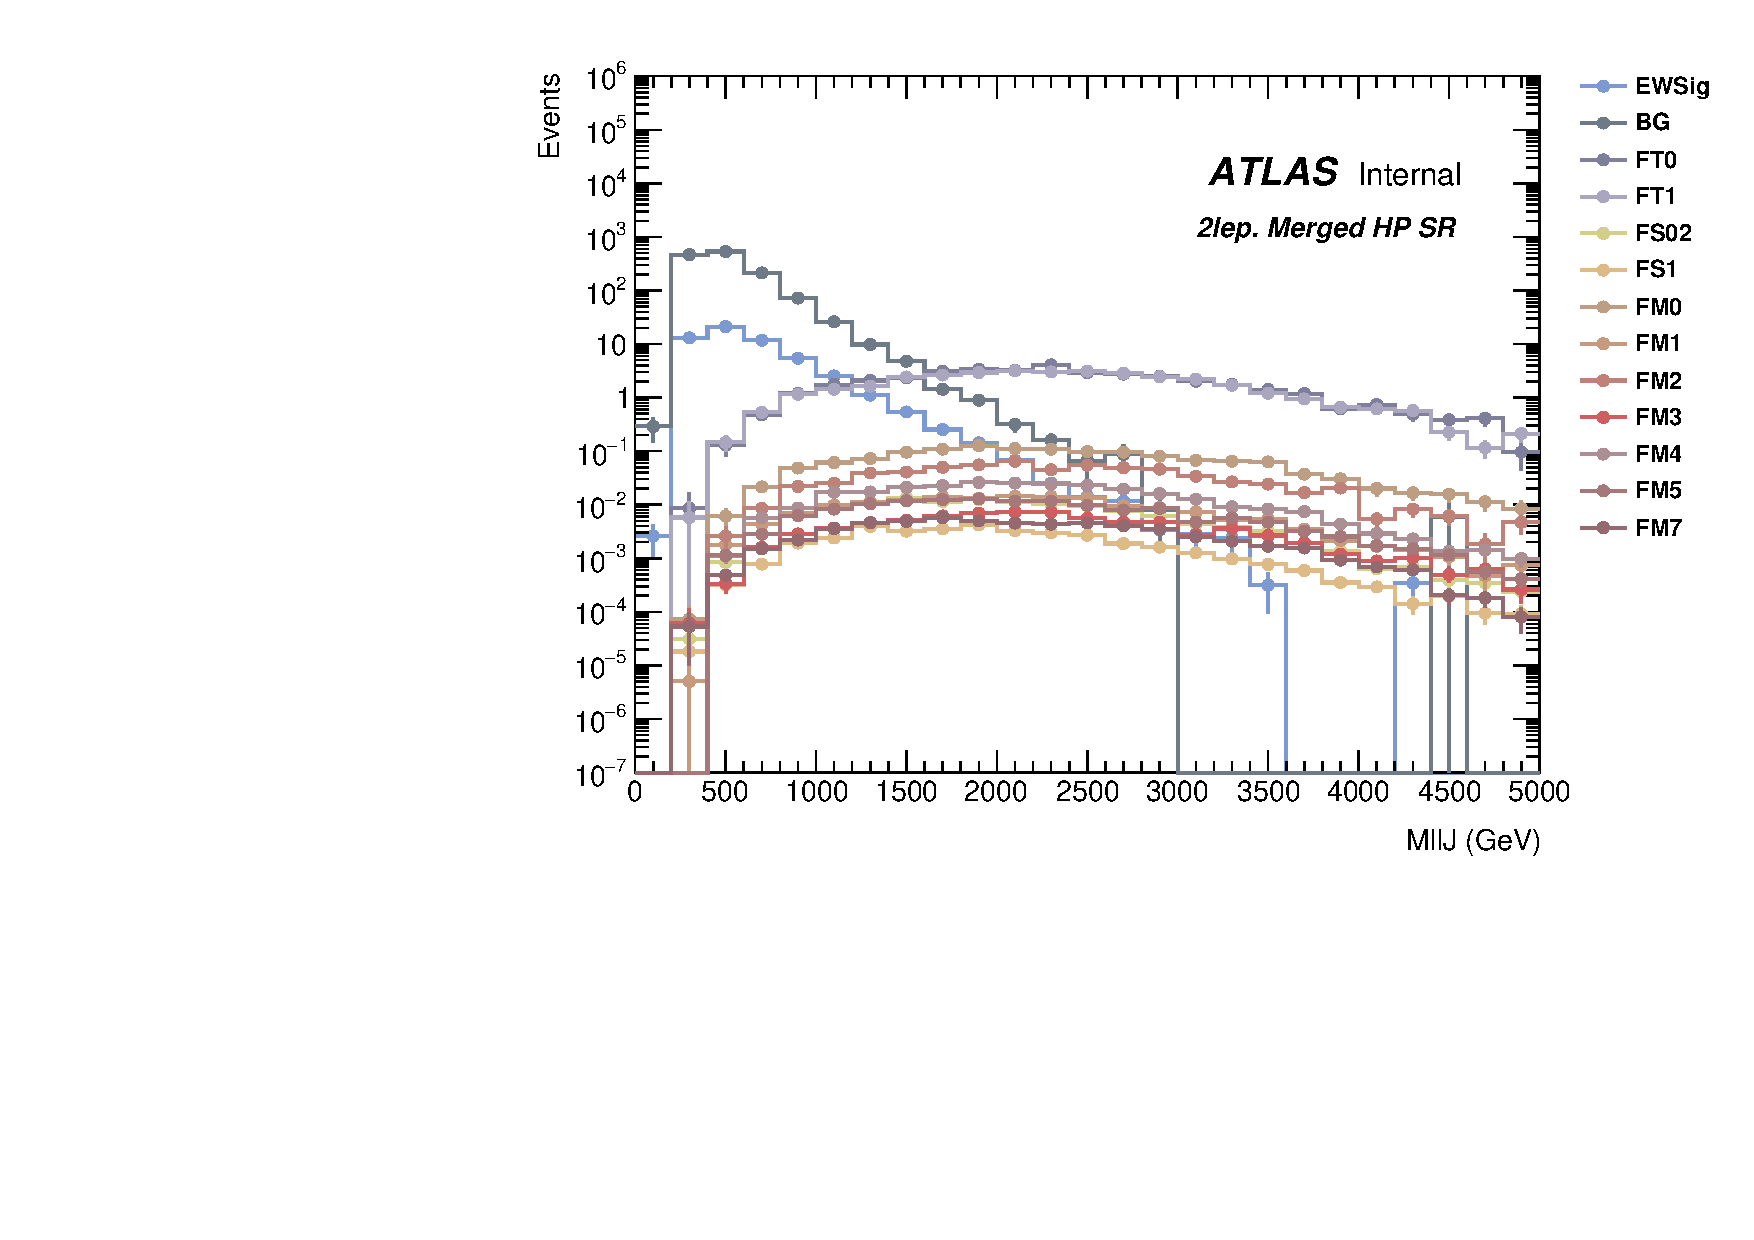
\includegraphics[width=0.45\textwidth]{figures/aQGC/MllJ_SR_HP_aQGC.pdf}}
    \subfigure[$m_{VV}$ distribution in Merged LP Signal region]{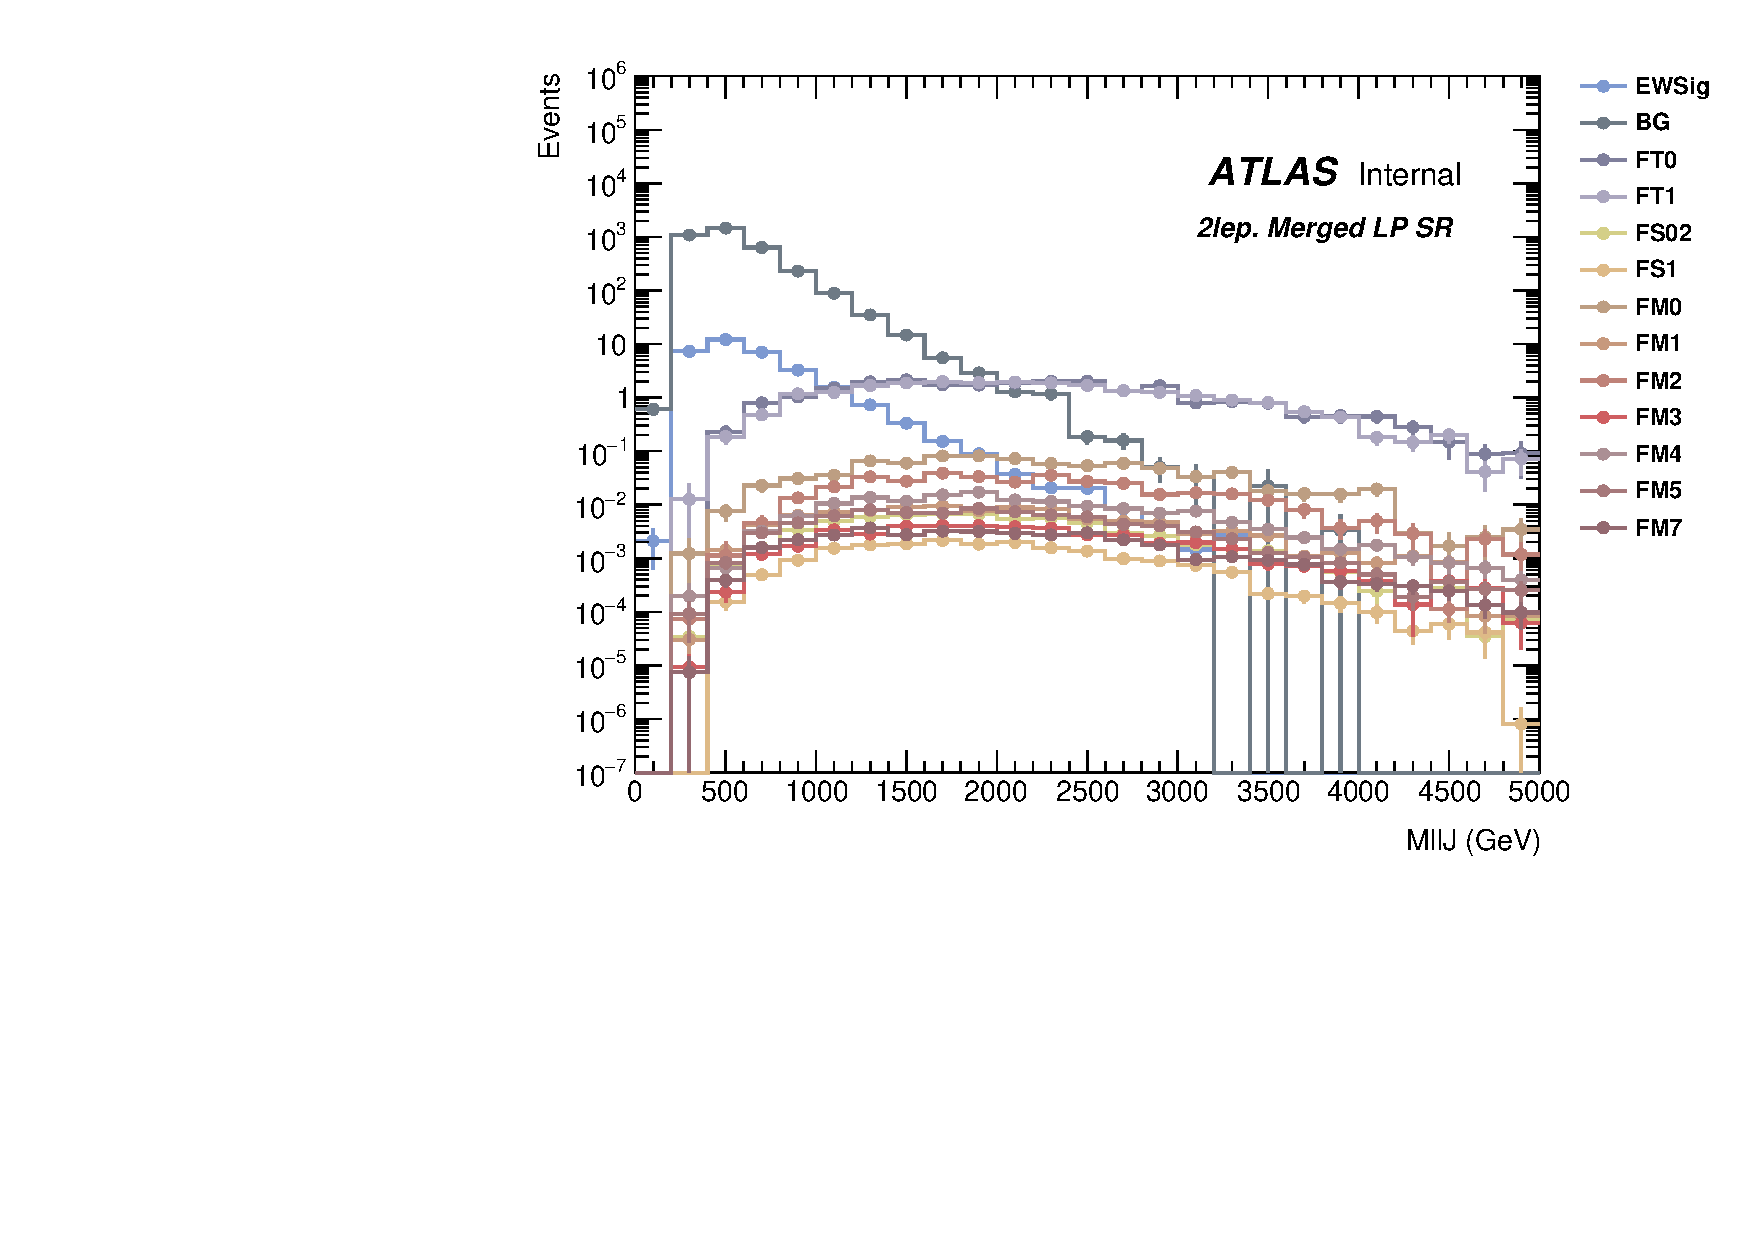
\includegraphics[width=0.45\textwidth]{figures/aQGC/MllJ_SR_LP_aQGC.pdf}}
    \caption{$m_{VV}$ shape distribution of each Wilson coefficient in Merged Signal regions. Only quadratic terms are shown.}
    \label{fig:2lepaQGCshapeMVV}
\end{figure}

\begin{figure}[ht]
    \centering
    \subfigure[RNN score distribution in Merged HP Signal region]{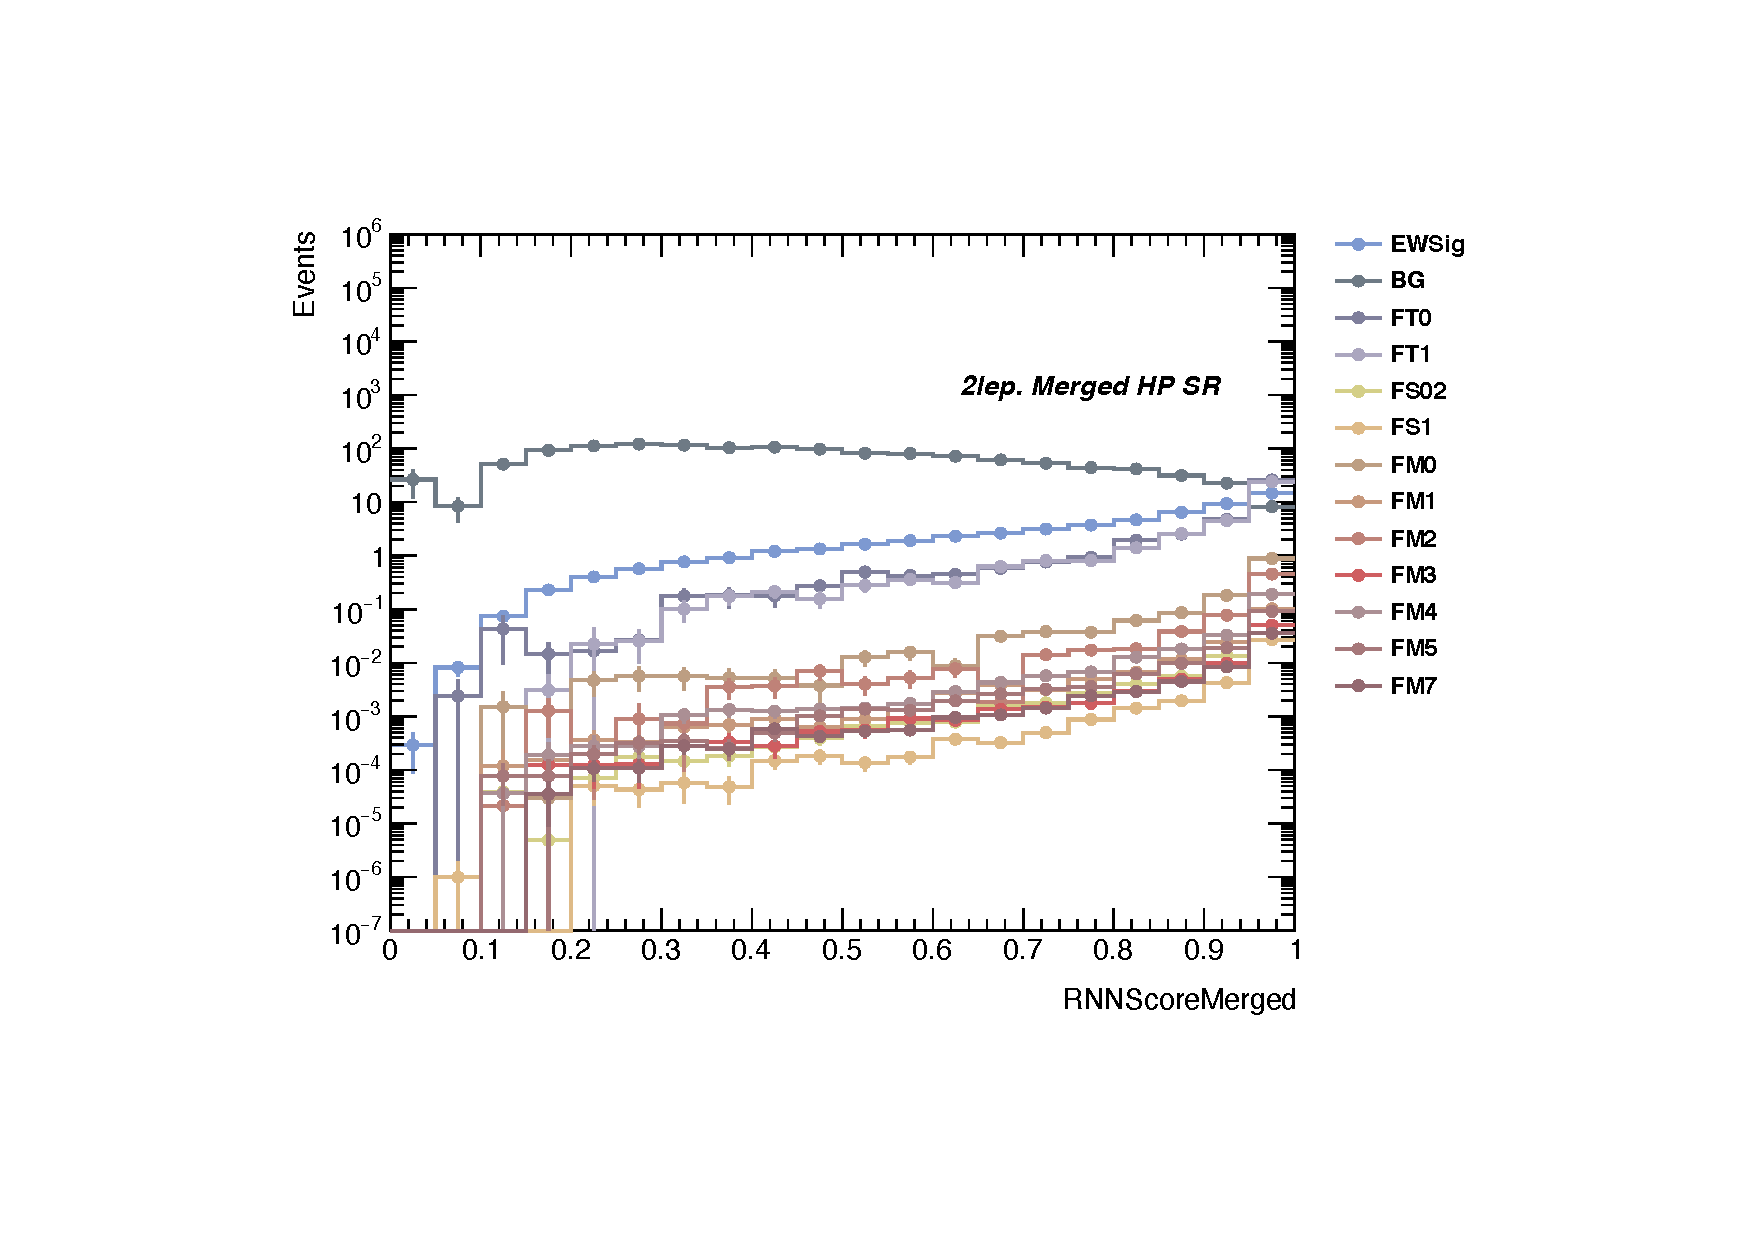
\includegraphics[width=0.45\textwidth]{figures/aQGC/RNNScoreMerged_SR_HP_aQGC.pdf}}
    \subfigure[RNN score distribution in Merged LP Signal region]{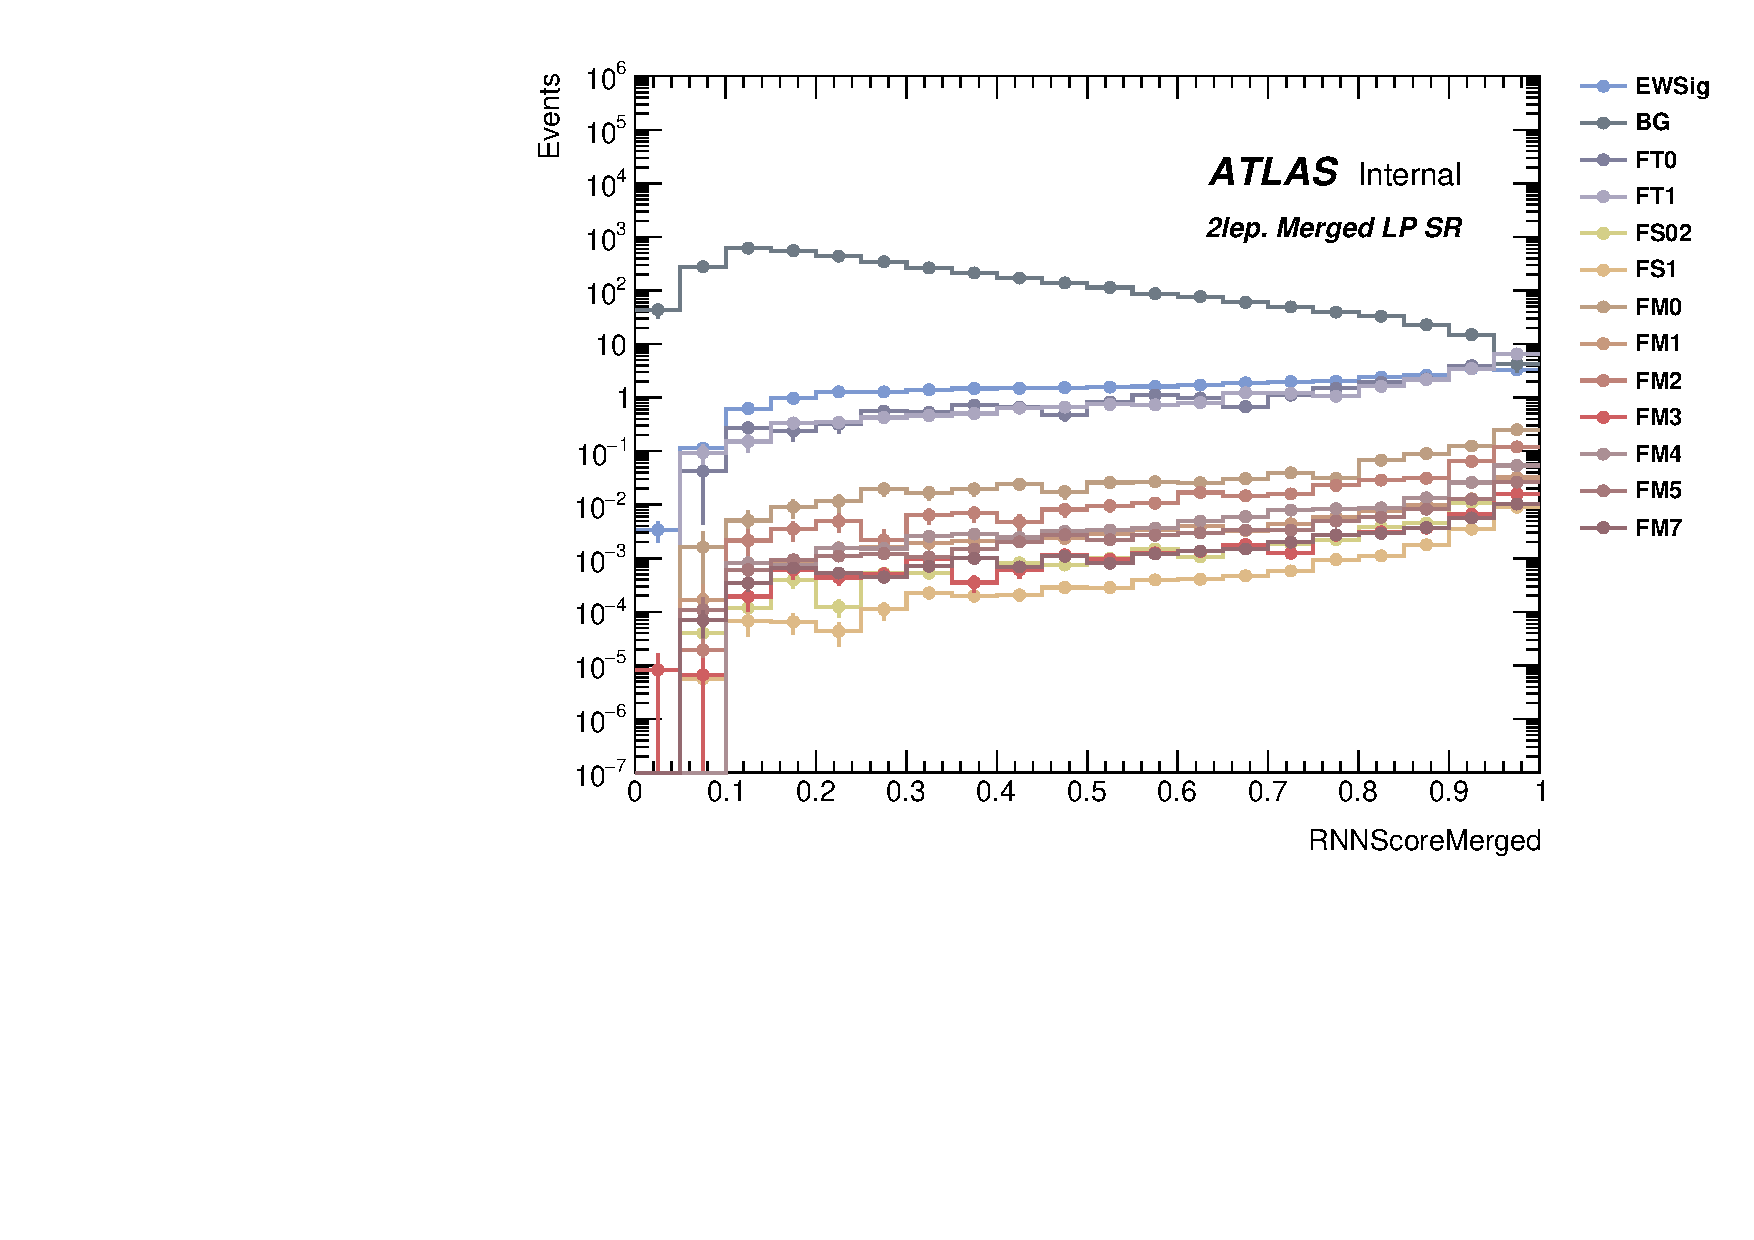
\includegraphics[width=0.45\textwidth]{figures/aQGC/RNNScoreMerged_SR_LP_aQGC.pdf}}
    \caption{RNN score shape distribution of each Wilson coefficient in Merged Signal regions. Only quadratic terms are shown.}
    \label{fig:2lepaQGCshapeRNN}
\end{figure}

The significance considering both $m_{VV}$ and RNNSCore distributions is tested here.
The binned significance defined as:
%
\begin{eqnarray*}
  Z = \sqrt{\sum_{bins}\left[2(s + b)ln\left(\frac{(s + b)(b+\sigma^2_{b})}{b^2+(s+b)\sigma^2_{b}}\right) - \frac{b^2}{\sigma^2_{b}}ln\left(1+\frac{\sigma^2_{b}s}{b(b+\sigma^2_{b})}\right)\right]} \\
\end{eqnarray*}
%
is used in this study.
The $s$ here refers to the number of the aQGC signal for the given Wilson coefficient.
The $b$ includes the SM electroweak signals and the other backgrounds (like Z+jets, ttbar, Diboson).
The fractional systematic uncertainty $\sigma_{b} = 0.2$ is assumed.

Two approaches are tested.
One is to use the $m_{VV}$ distribution for the binned significance definition, after the cut on the RNNScore.
The other is to use the RNNScore distribution for the binned significance calculation, after the cut on the $m_{VV}$.

Figure~\ref{fig:2lepaQGCBinnedSigMVV} shows the binned significance using $m_{VV}$ distribution,
as functions of the cut thresholds of RNNSCore and $\mathrm{M}_{tagjj}$.
No cuts on RNNScore and $\mathrm{M}_{tagjj}$ are preferred, in particular for the FT0 term.

Figure~\ref{fig:2lepaQGCBinnedSigRNN} shows the binned significance using RNNScore distribution
as functions of the cut thresholds for $m_{VV}$ and $\mathrm{M}_{tagjj}$.
It is preferred to apply the cut on $m_{VV}$ if we want to use RNNScore as the discriminant.

The significance value for each Wilson coefficient term is summarized in tables~\ref{tab:2lep_HPSR_MVV} and \ref{tab:2lep_HPSR_RNN}.

\begin{figure}[ht]
    \centering
    	\subfigure[ FT0 term ]{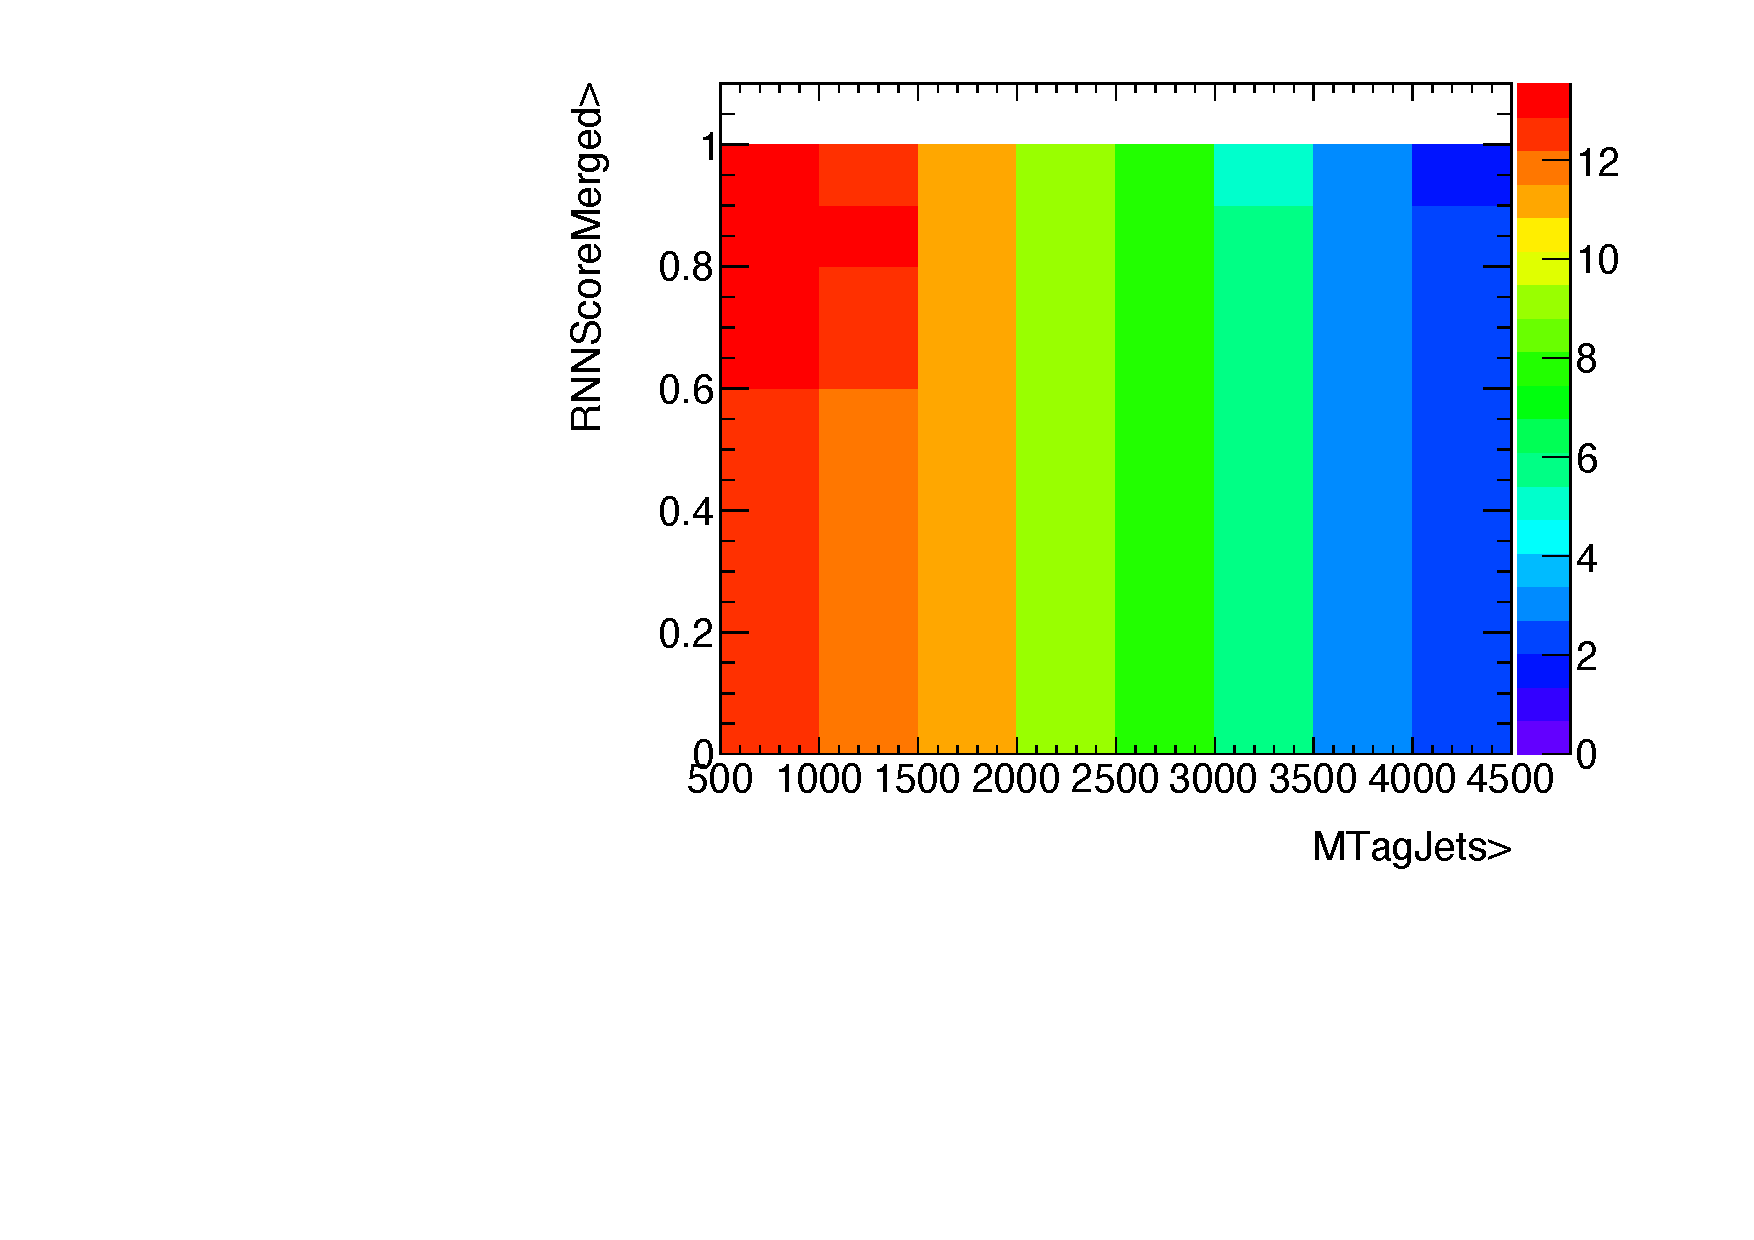
\includegraphics[width=0.30\textwidth]{figures/aQGC/HPSRFT0MVV.pdf}}
    	\subfigure[ FS02 term]{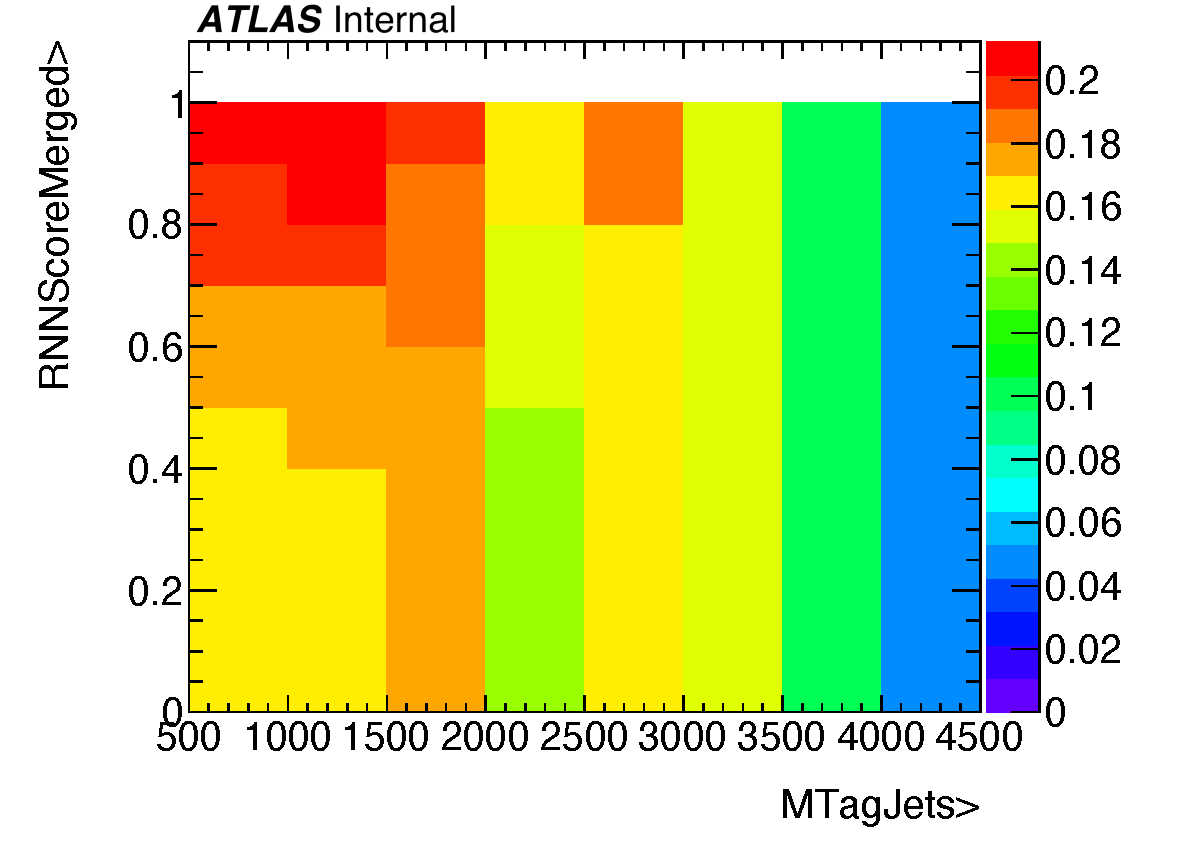
\includegraphics[width=0.30\textwidth]{figures/aQGC/HPSRFS02MVV.pdf}}
    	\subfigure[ FM0 term ]{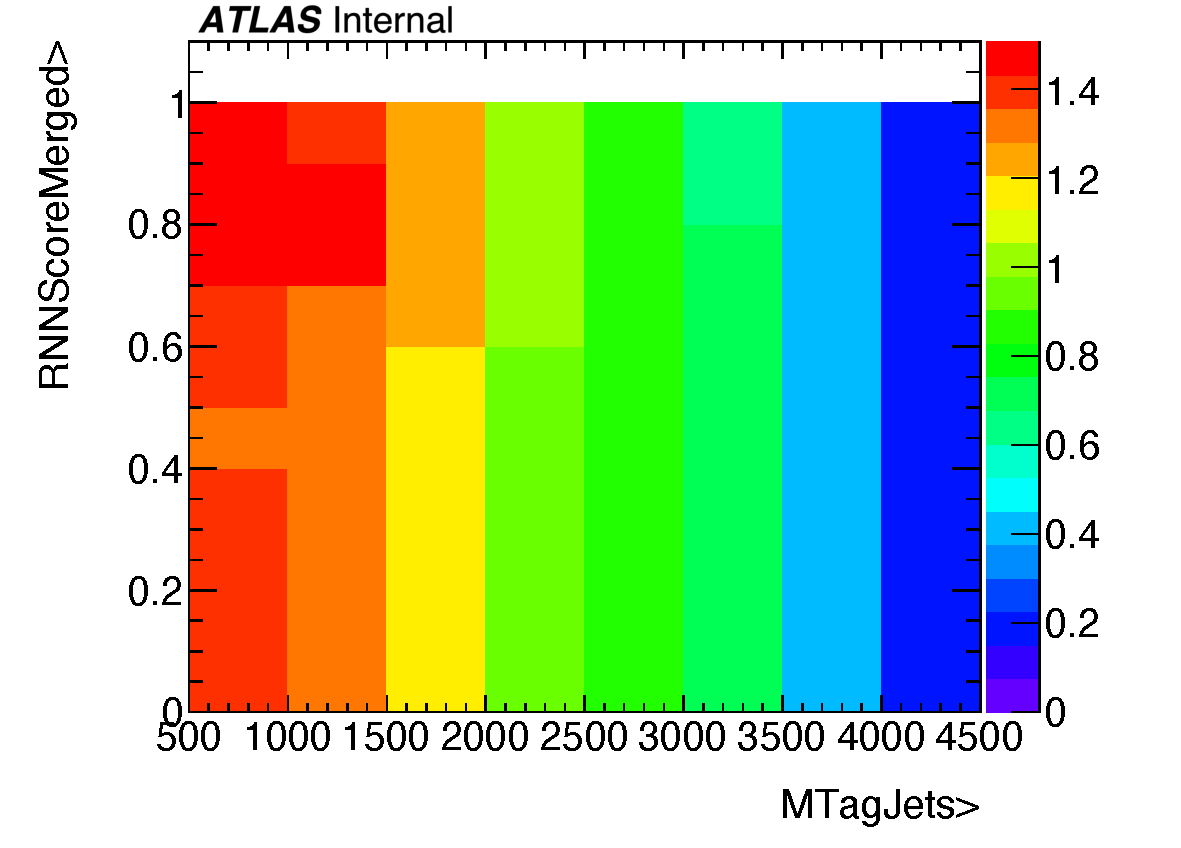
\includegraphics[width=0.30\textwidth]{figures/aQGC/HPSRFM0MVV.pdf}}
        \caption{The 2D scan of the binned significance of operator FT0 (left), FS02 (middle), FM0 (right) with $m_{VV}$ score as discriminant in Merged HP signal region. Only quadratic terms are scanned.}
        \label{fig:2lepaQGCBinnedSigMVV}
\end{figure}

\begin{figure}[ht]
    \centering
    	\subfigure[ FT0 term ]{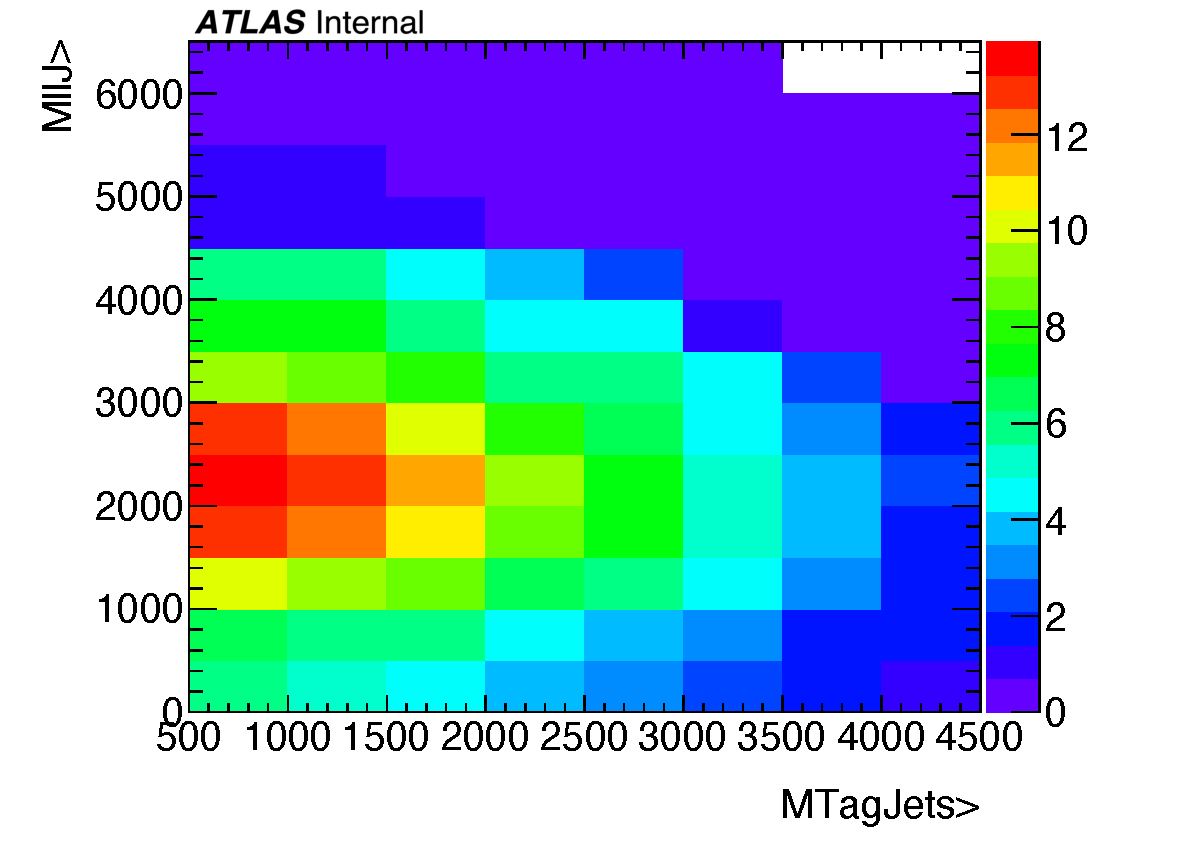
\includegraphics[width=0.30\textwidth]{figures/aQGC/HPSRFT0RNN.pdf}}
    	\subfigure[ FS02 term]{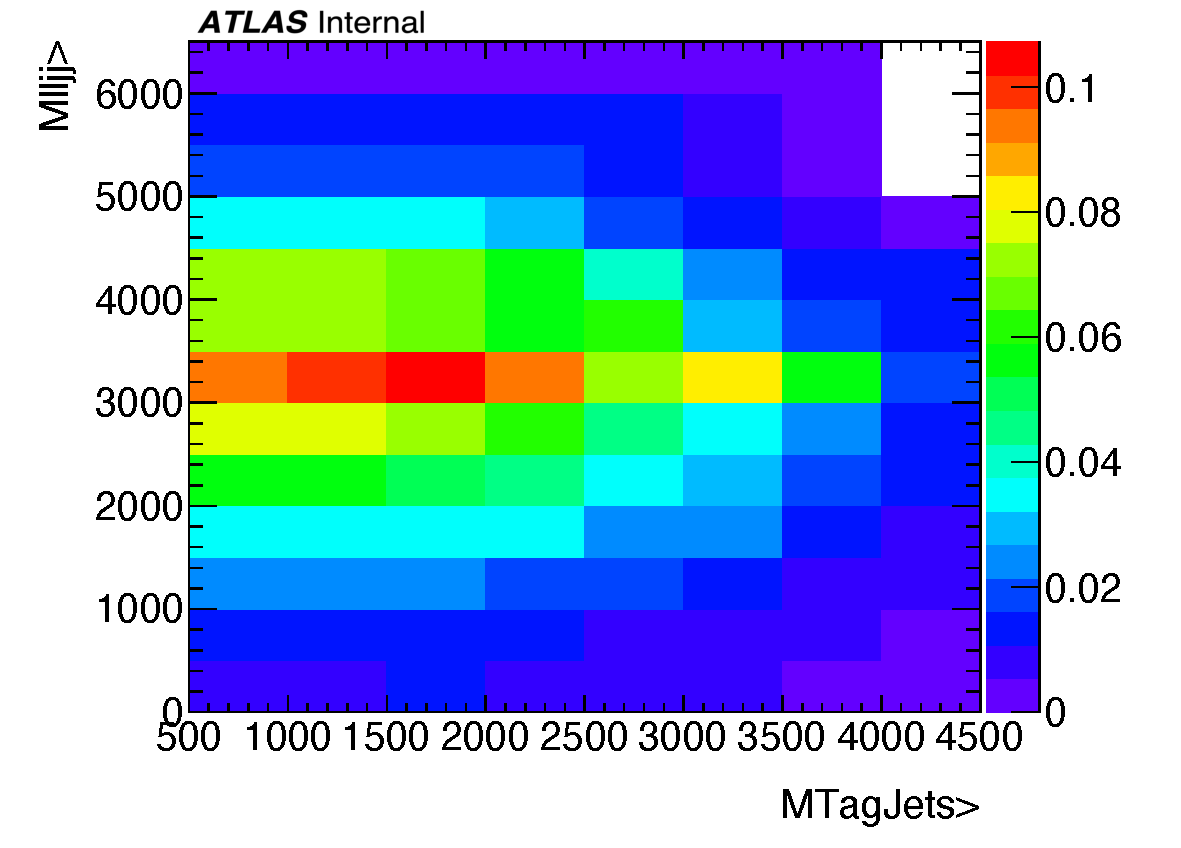
\includegraphics[width=0.30\textwidth]{figures/aQGC/HPSRFS02RNN.pdf}}
    	\subfigure[ FM0 term ]{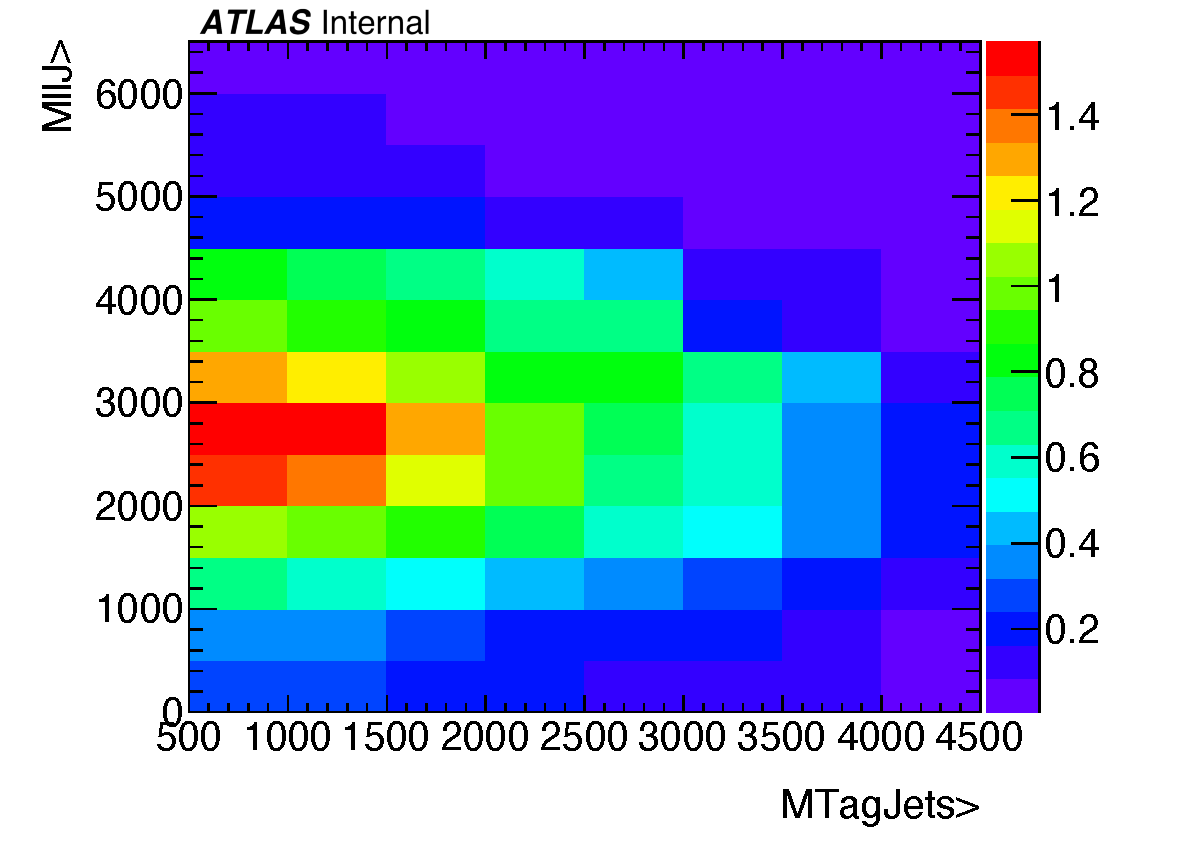
\includegraphics[width=0.30\textwidth]{figures/aQGC/HPSRFM0RNN.pdf}}
        \caption{The 2D scan of the binned significance of operator FT0 (left), FS02 (middle), FM0 (right) with RNN score as discriminant in Merged HP signal region. Only quadratic terms are scanned.}
        \label{fig:2lepaQGCBinnedSigRNN}
\end{figure}

\clearpage

\begin{table}[ht!]
\small
\begin{center}
\resizebox{0.50\textwidth}{!}{

 \begin{tabular}{ r ||  r  r  r  r  |}
    & $\mathrm{M}_{tagjj}$ (GeV) & RNN score  & significance before cut& significance  \tabularnewline \hline
FT0 & 500                        & 0.6        & 12.55                  & 12.98         \tabularnewline \hline
FT1 & 500                        & 0.6        & 11.94                  & 12.50         \tabularnewline \hline
FS02& 1000                       & 0.8        & 0.17                   & 0.20          \tabularnewline \hline
FS1 & 500                        & 0.8        & 0.07                   & 0.07          \tabularnewline \hline
FM0 & 500                        & 0.7        & 1.36                   & 1.50          \tabularnewline \hline
FM1 & 500                        & 0.3        & 0.25                   & 0.27          \tabularnewline \hline
FM2 & 500                        & 0.7        & 0.82                   & 0.93          \tabularnewline \hline
FM3 & 500                        & 0.6        & 0.15                   & 0.16          \tabularnewline \hline
FM4 & 500                        & 0.7        & 0.38                   & 0.42          \tabularnewline \hline
FM5 & 500                        & 0.7        & 0.23                   & 0.25          \tabularnewline \hline
FM7 & 500                        & 0.6        & 0.12                   & 0.12          \tabularnewline \hline

\end{tabular}
}
\caption{Best cut point table for binned significance for $m_{VV}$ score distribution in \tlep channel in HPSR}
\label{tab:2lep_HPSR_MVV}
\end{center}
\end{table}

\begin{table}[ht!]
\small
\begin{center}
\resizebox{0.50\textwidth}{!}{

 \begin{tabular}{ r ||  r  r  r  r  |}
    & $\mathrm{M}_{tagjj}$ (GeV) & RNN score  & significance before cut & significance \tabularnewline \hline
FT0 & 500          & 0.1  & 6.65      & 6.77                          \tabularnewline \hline
FT1 & 500          & 0.2  & 6.69      & 6.85                          \tabularnewline \hline
FS02& 500          & 0.9  & 0.05      & 0.10                          \tabularnewline \hline
FS1 & 1000         & 0.8  & 0.02      & 0.04                          \tabularnewline \hline
FM0 & 500          & 0.8  & 0.54      & 0.12                          \tabularnewline \hline
FM1 & 500          & 0.1  & 0.08      & 0.42                          \tabularnewline \hline
FM2 & 500          & 0.9  & 0.28      & 0.08                          \tabularnewline \hline
FM3 & 1000         & 0.8  & 0.05      & 0.18                          \tabularnewline \hline
FM4 & 1000         & 0.8  & 0.12      & 0.10                          \tabularnewline \hline
FM5 & 1000         & 0.8  & 0.07      & 0.10                          \tabularnewline \hline
FM7 & 500          & 0.1  & 0.04      & 0.06                          \tabularnewline \hline

\end{tabular}
}
\caption{Best cut point table for binned significance for $m_{VV}$ score distribution in \tlep channel in LPSR}
\label{tab:2lep_LPSR_MVV}
\end{center}
\end{table}

\begin{table}[ht!]
\small
\begin{center}
\resizebox{0.50\textwidth}{!}{

 \begin{tabular}{ r ||  r  r  r  r  |}
    & $\mathrm{M}_{tagjj}$ (GeV) & MllJ (GeV) & significance before cut& significance \tabularnewline \hline
FT0 & 500          & 2000   & 5.62    & 13.92                           \tabularnewline \hline
FT1 & 500          & 2000   & 5.25    & 13.31                           \tabularnewline \hline
FS02& 1500         & 3000   & 0.01    & 0.11                            \tabularnewline \hline
FS1 & 2500         & 3000   & 0.01    & 0.07                            \tabularnewline \hline
FM0 & 500          & 2500   & 0.27    & 1.57                            \tabularnewline \hline
FM1 & 500          & 2500   & 0.03    & 0.28                            \tabularnewline \hline
FM2 & 500          & 2500   & 0.14    & 0.95                            \tabularnewline \hline
FM3 & 500          & 3000   & 0.01    & 0.12                            \tabularnewline \hline
FM4 & 500          & 2500   & 0.06    & 0.45                            \tabularnewline \hline
FM5 & 500          & 2500   & 0.03    & 0.25                            \tabularnewline \hline
FM7 & 500          & 2500   & 0.01    & 0.12                            \tabularnewline \hline

\end{tabular}
}
\caption{Best cut point table for binned significance for RNN score distribution in \tlep channel in HPSR}
\label{tab:2lep_HPSR_RNN}
\end{center}
\end{table}

\begin{table}[ht!]
\small
\begin{center}
\resizebox{0.50\textwidth}{!}{

 \begin{tabular}{ r ||  r  r  r  r  |}
    & $\mathrm{M}_{tagjj}$ (GeV) & MllJ (GeV) & significance before cut& significance \tabularnewline \hline
FT0 & 500          & 2000  & 2.64     & 7.72                            \tabularnewline \hline
FT1 & 500          & 2000  & 2.80     & 7.46                            \tabularnewline \hline
FS02& 1500         & 3000  & 0.01     & 0.06                            \tabularnewline \hline
FS1 & 500          & 3000  & 0.00     & 0.06                            \tabularnewline \hline
FM0 & 500          & 2500  & 0.12     & 0.92                            \tabularnewline \hline
FM1 & 500          & 3000  & 0.02     & 0.18                            \tabularnewline \hline
FM2 & 500          & 3000  & 0.06     & 0.54                            \tabularnewline \hline
FM3 & 500          & 3000  & 0.01     & 0.12                            \tabularnewline \hline
FM4 & 500          & 3000  & 0.03     & 0.26                            \tabularnewline \hline
FM5 & 500          & 3000  & 0.01     & 0.16                            \tabularnewline \hline
FM7 & 500          & 3000  & 0.01     & 0.09                            \tabularnewline \hline

\end{tabular}
}
\caption{Best cut point table for binned significance for RNN score distribution in \tlep channel LPSR}
\label{tab:2lep_LPSR_RNN}
\end{center}
\end{table}

Comparing the significance between table~\ref{tab:2lep_HPSR_MVV} and table~\ref{tab:2lep_HPSR_RNN}, 
RNN score as discriminant with $m_{VV}$ cut around 2.5~TeV shows slightly better but not so different ability with the $m_{VV}$ without any cut.
It seems to be the simple and better way to use $m_{VV}$ as the discriminant without cut. 

Following the study of this section, the profile likelihood fit with $m_{VV}$ score is performed and the expected limit is shown in section~\ref{subsec:aqgc_limit}. The fit study with RNN score as discriminant is also shown in section~\ref{subsec:2binapproach}.

\subsection{Expected limit}
\label{subsec:aqgc_limit}

The expected upper limit on each Wilson coefficient by a combined fit of all 3 channels is shown in table~\ref{tab:aQGC_limit}, which is calculated by $\sqrt{\mu_{95\%}} = f_{i} / \Lambda^4$, where $\mu_{95\%}$ is the 95\% upper limit on the signal strength.
The $m_{VV}$ distributions without any additional cuts are used in the fit.
The systematic uncertainties are yet to be included.
Figures~\ref{fig:0lepFT0} and ~\ref{fig:1lepFT0}, ~\ref{fig:2lepFT0} show the prefit plots of $m_{VV}$ distribution. FT0 signal is overlaid.

\begin{table}[ht!]
\small
\begin{center}
\resizebox{0.30\textwidth}{!}{
 \begin{tabular}{ | r || r |}
    & Expected limit (TeV$^{-4})$ \tabularnewline \hline
FT0 & 0.14                        \tabularnewline \hline
FT1 & 0.14                        \tabularnewline \hline
FS02& 2.90                        \tabularnewline \hline
FS1 & 4.56e+6                     \tabularnewline \hline
FM0 & 0.85                        \tabularnewline \hline
FM1 & 2.55                        \tabularnewline \hline
FM2 & 1.26                        \tabularnewline \hline
FM3 & 4.69e+2                     \tabularnewline \hline
FM4 & 2.07                        \tabularnewline \hline
FM5 & 81.3                        \tabularnewline \hline
FM7 & 5.37e+2                     \tabularnewline \hline
\end{tabular}
}
\caption{Expected upper limits of each Wilson coefficient. All 3 channels are combined.}
\label{tab:aQGC_limit}
\end{center}
\end{table}

\begin{figure}[ht]
    \centering
    	\subfigure[ 0lep merged CR ]{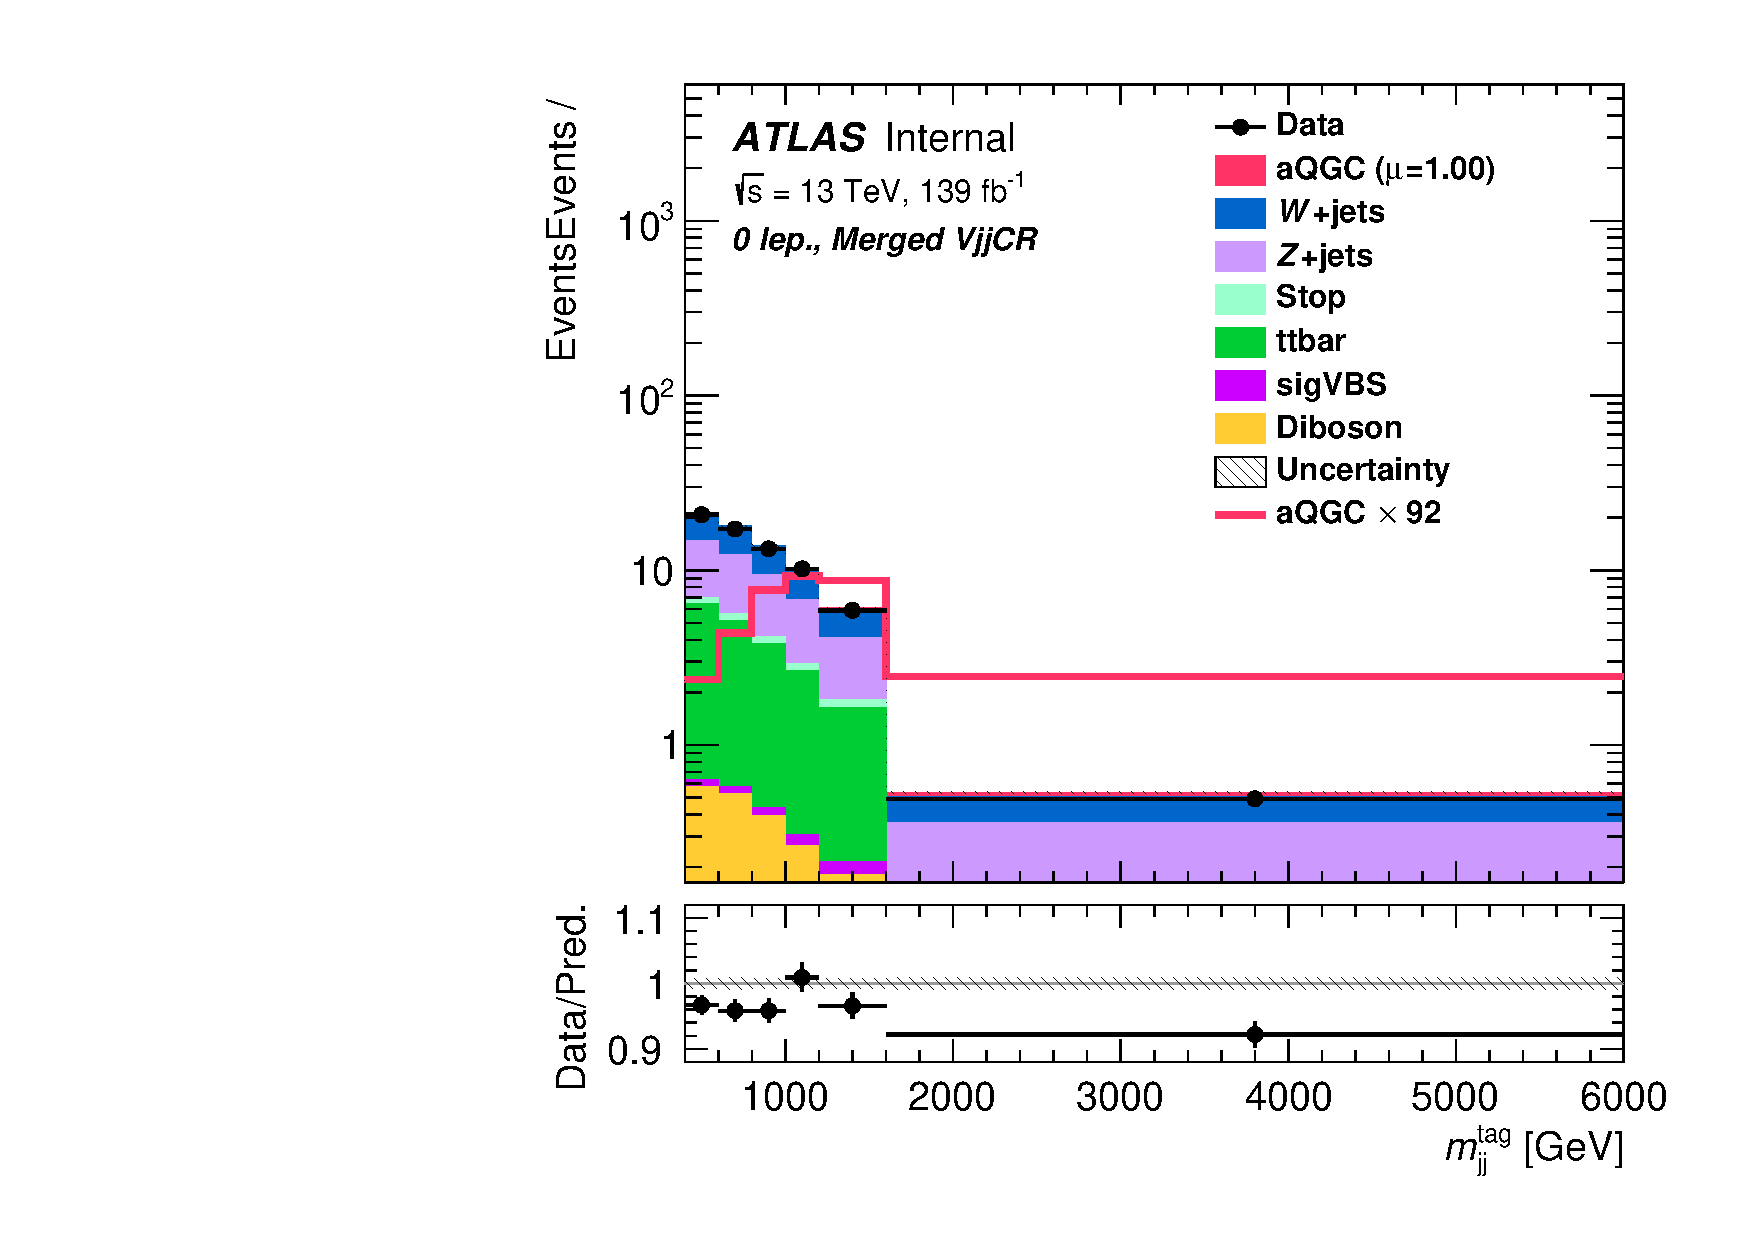
\includegraphics[width=0.32\textwidth]{figures/aQGC/Region_distMTagJets_DCRVjetMer_BMin0_J0_incJet1_L0_T0_incFat1_Y6051_incTag1_Fat1_Prefitlog.pdf}}
    	\subfigure[ 0lep HP SR ]{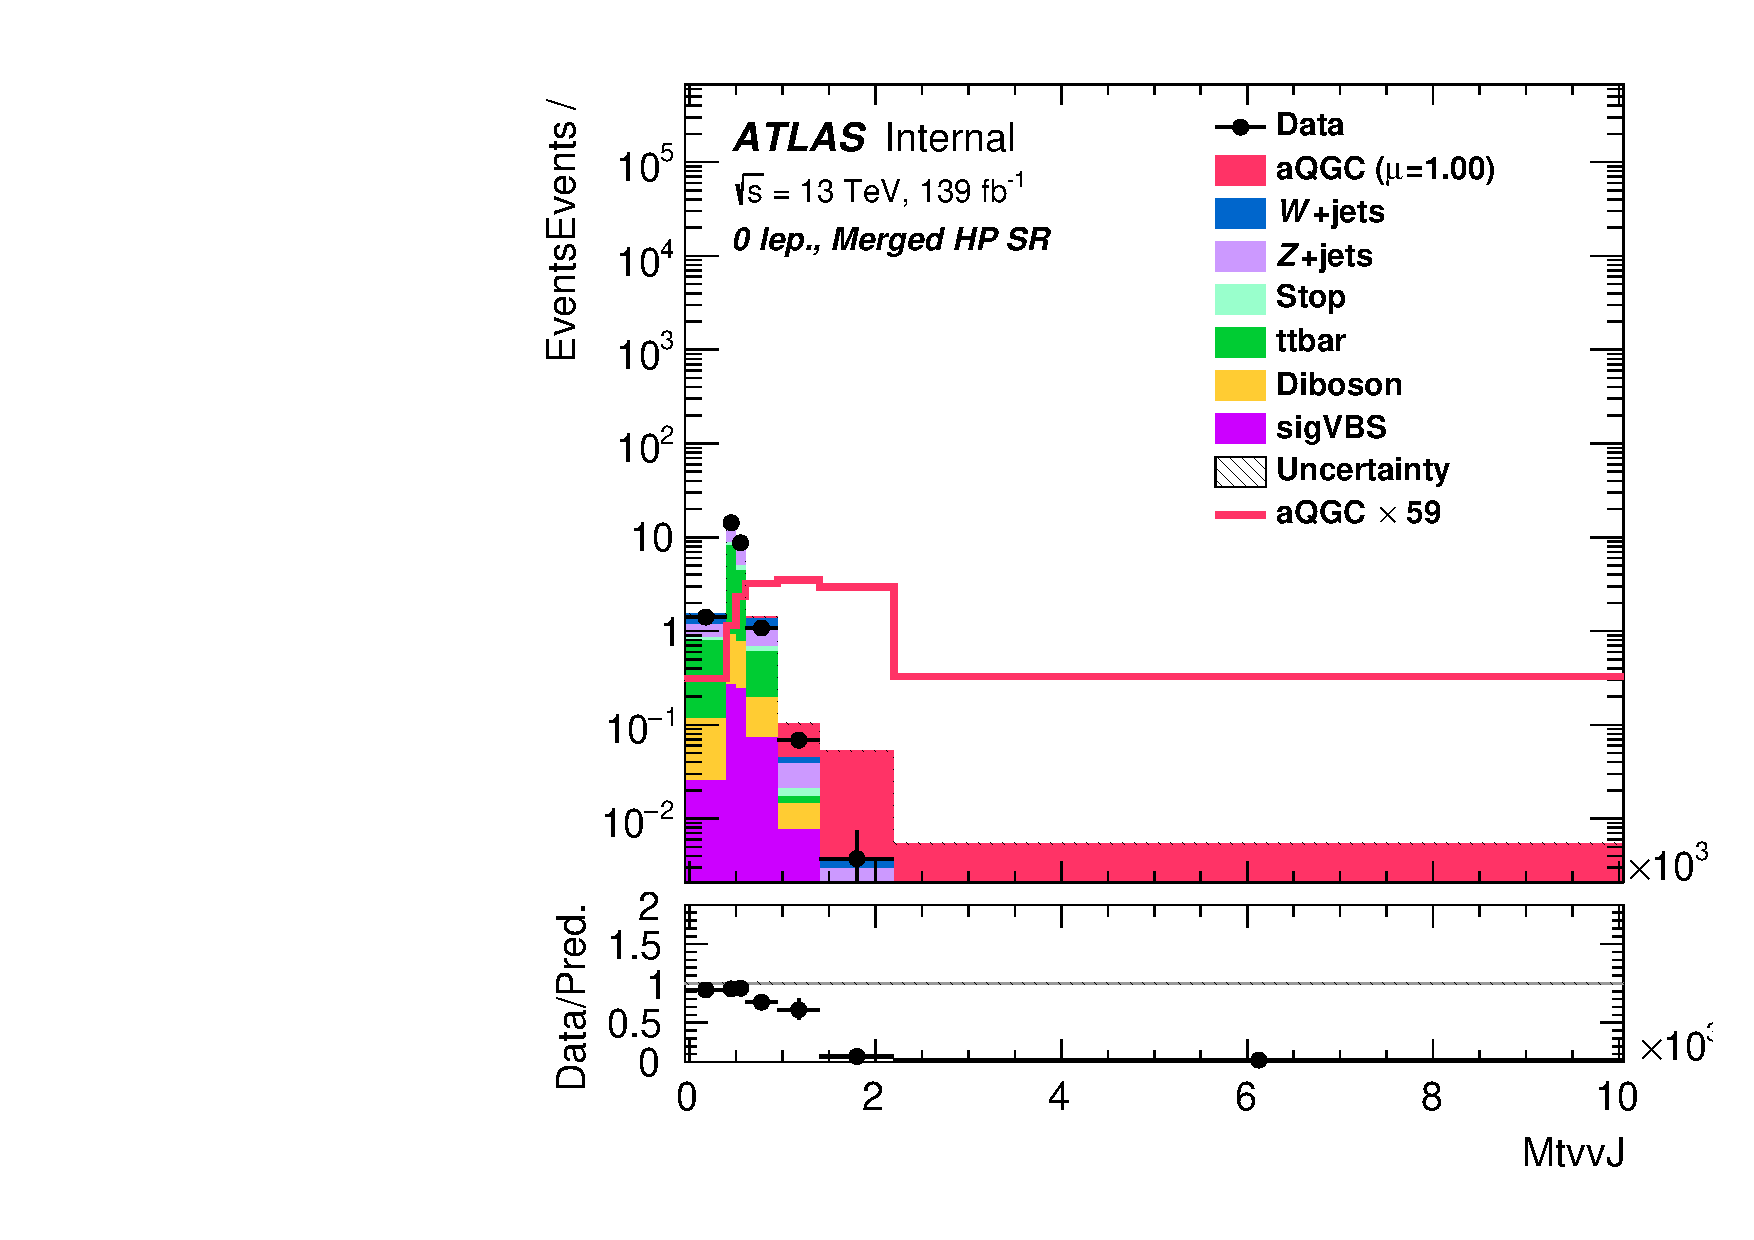
\includegraphics[width=0.32\textwidth]{figures/aQGC/Region_distMtvvJ_DSRVBSHP_BMin0_J0_incJet1_L0_T0_incFat1_Y6051_incTag1_Fat1_Prefitlog.pdf}}
    	\subfigure[ 0lep LP SR ]{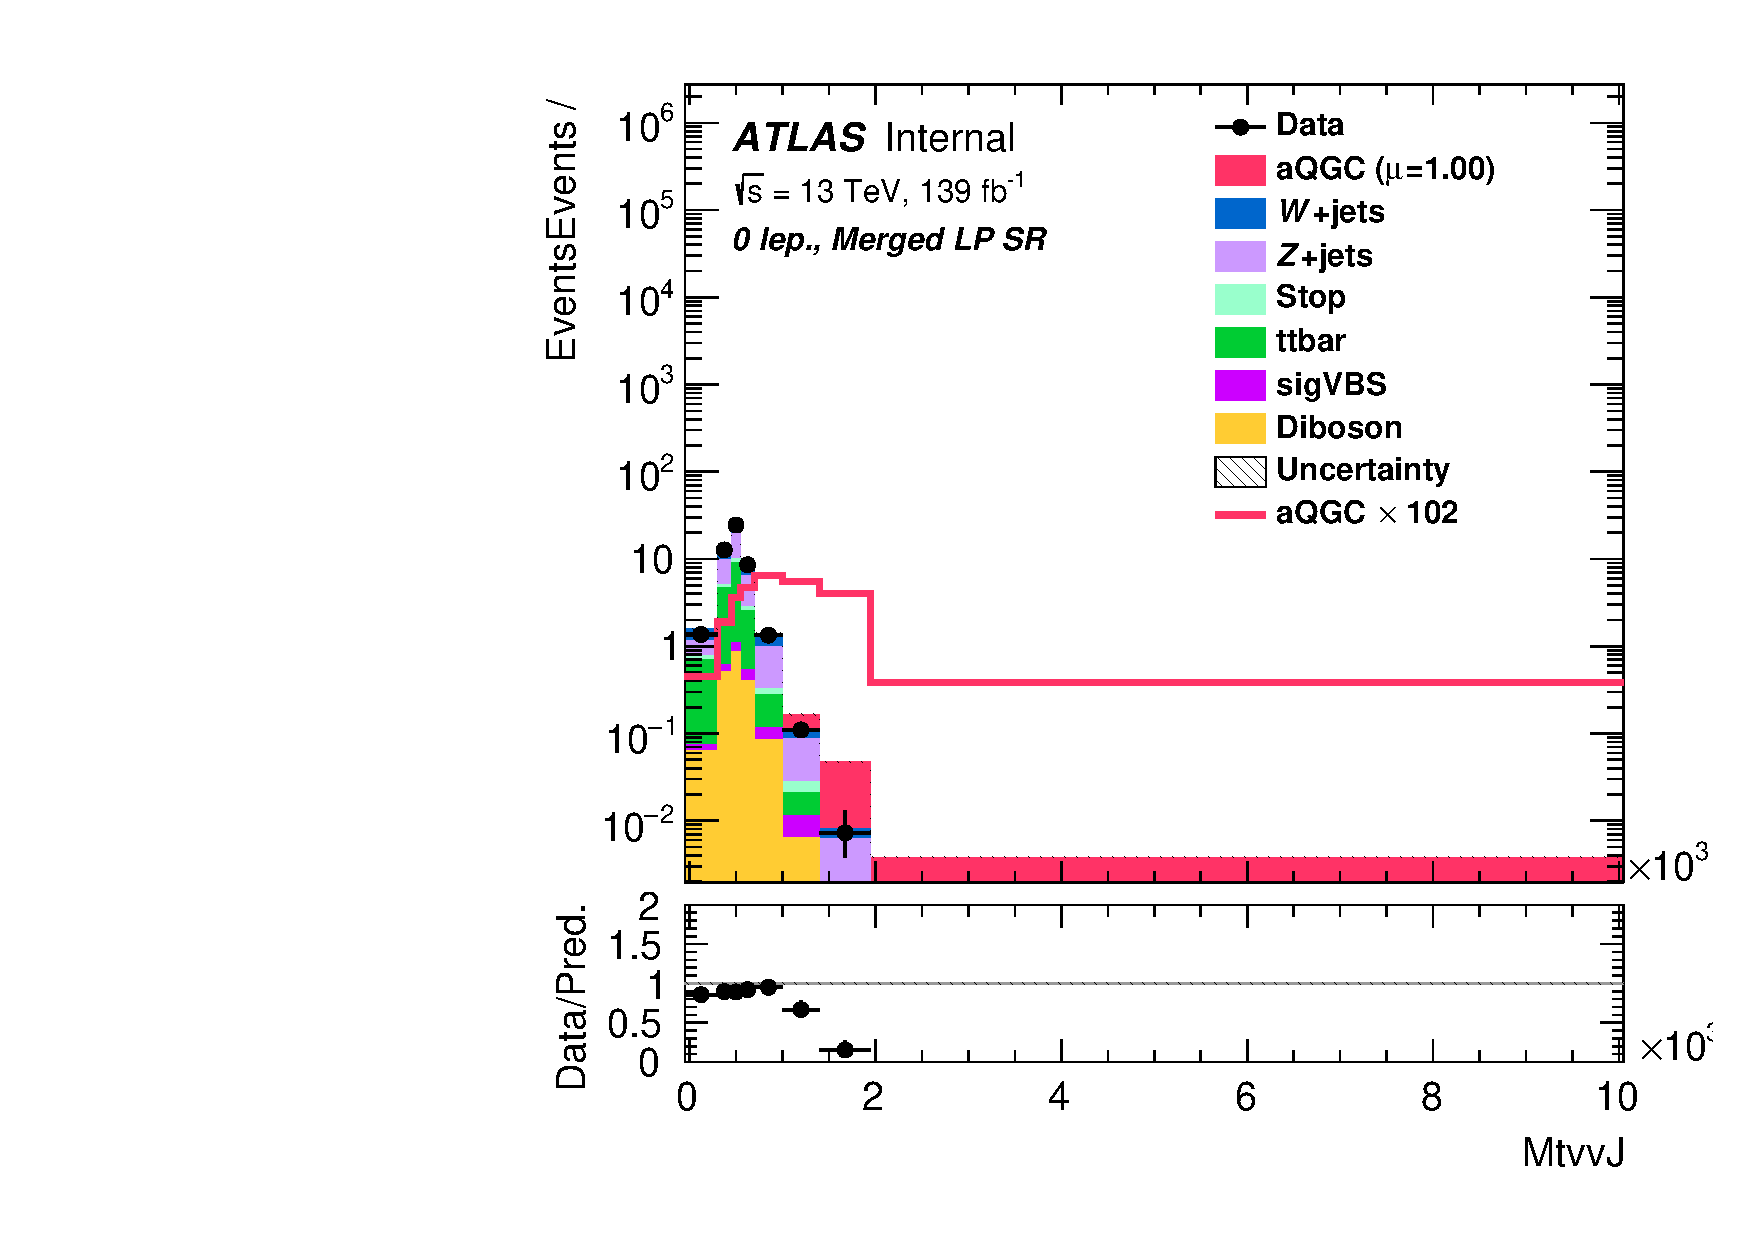
\includegraphics[width=0.32\textwidth]{figures/aQGC/Region_distMtvvJ_DSRVBSLP_BMin0_J0_incJet1_L0_T0_incFat1_Y6051_incTag1_Fat1_Prefitlog.pdf}}
    	\subfigure[ 0lep resolved CR ]{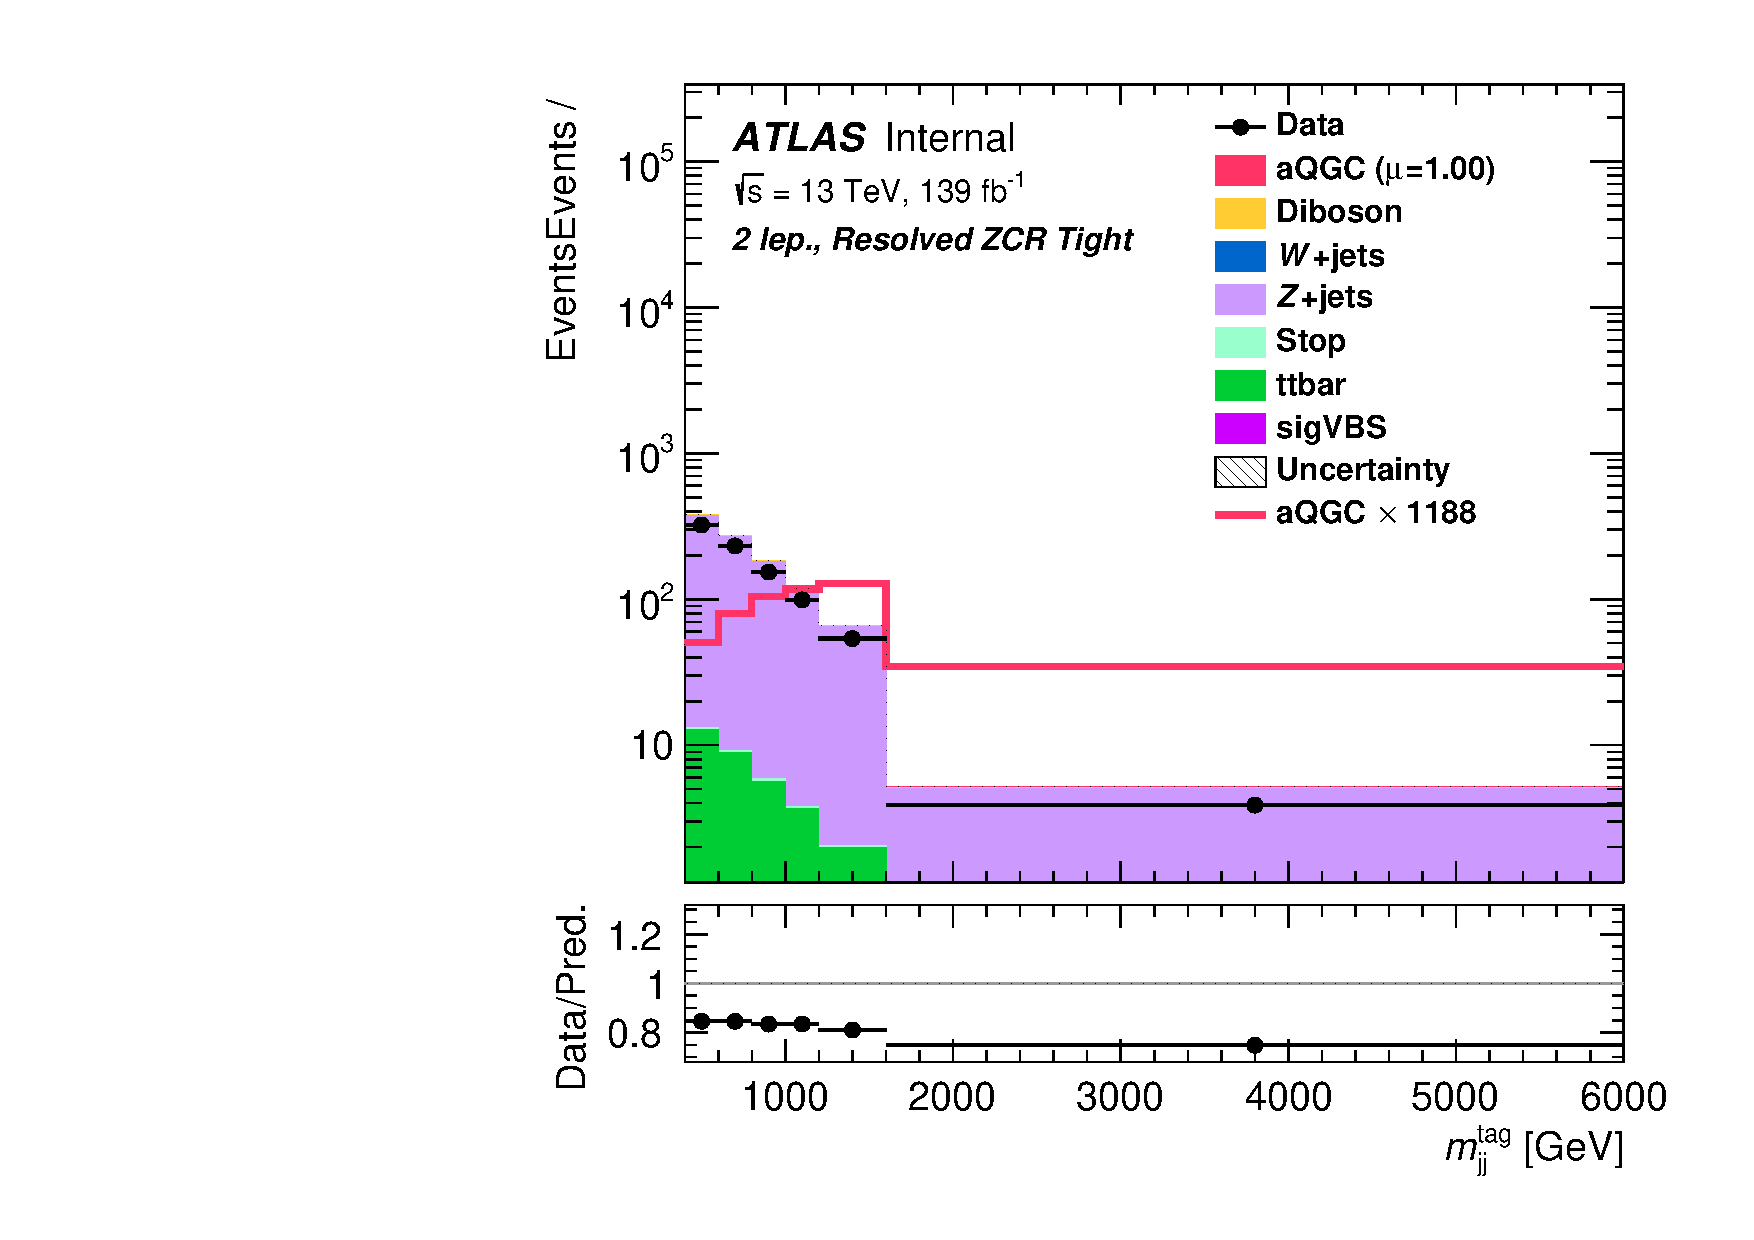
\includegraphics[width=0.32\textwidth]{figures/aQGC/Region_distMTagResJets_DCRVjetFid_BMin0_T0_Y6051_incTag1_J2_L2_incJet1_Prefitlog.pdf}}
    	\subfigure[ 0lep resolved SR ]{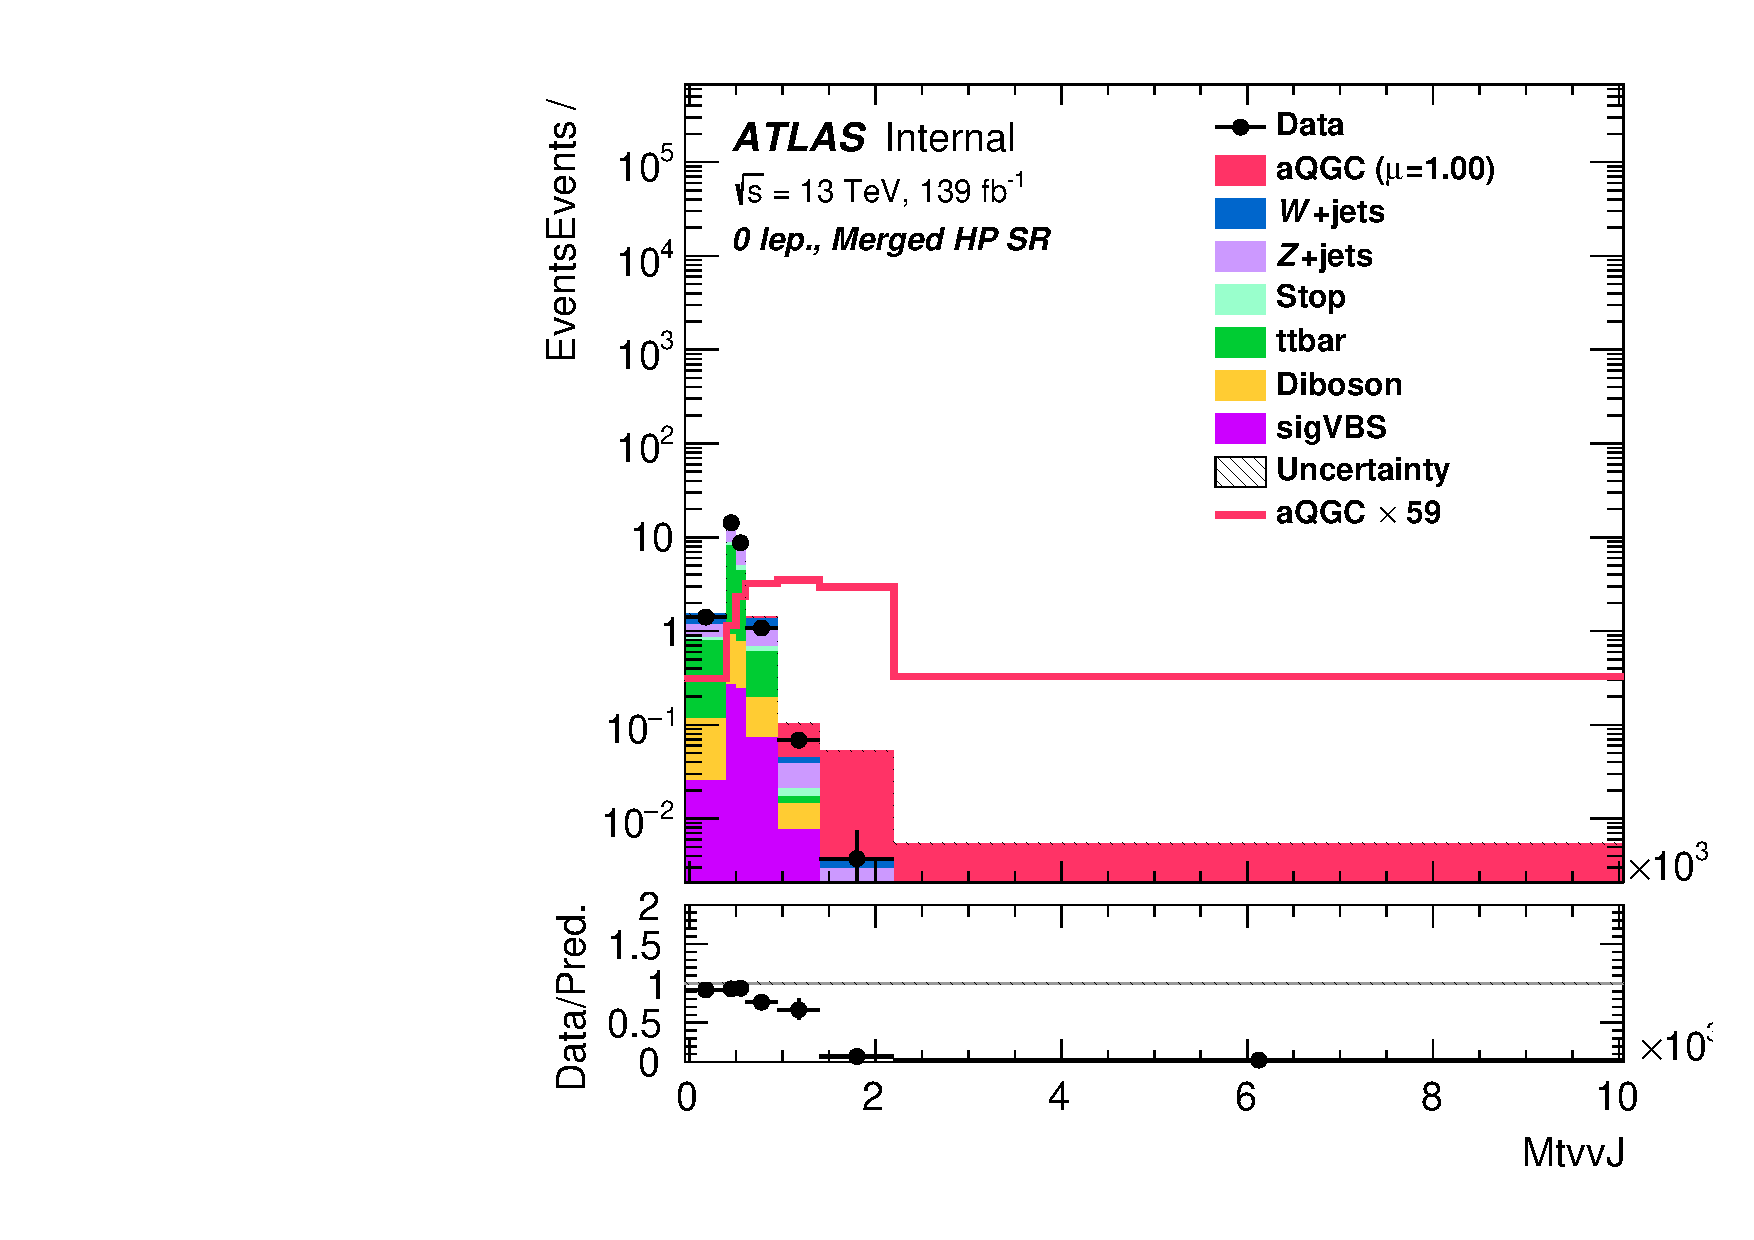
\includegraphics[width=0.32\textwidth]{figures/aQGC/Region_distMtvvJ_DSRVBSHP_BMin0_J0_incJet1_L0_T0_incFat1_Y6051_incTag1_Fat1_Prefitlog.pdf}}
        \caption{Prefit plots for operator FT0 in \zlep channel are shown. The standard model EW signal is floated as the background.}
        \label{fig:0lepFT0}
\end{figure}

\begin{figure}[ht]
    \centering
    	\subfigure[ 1lep merged Vjet CR ]{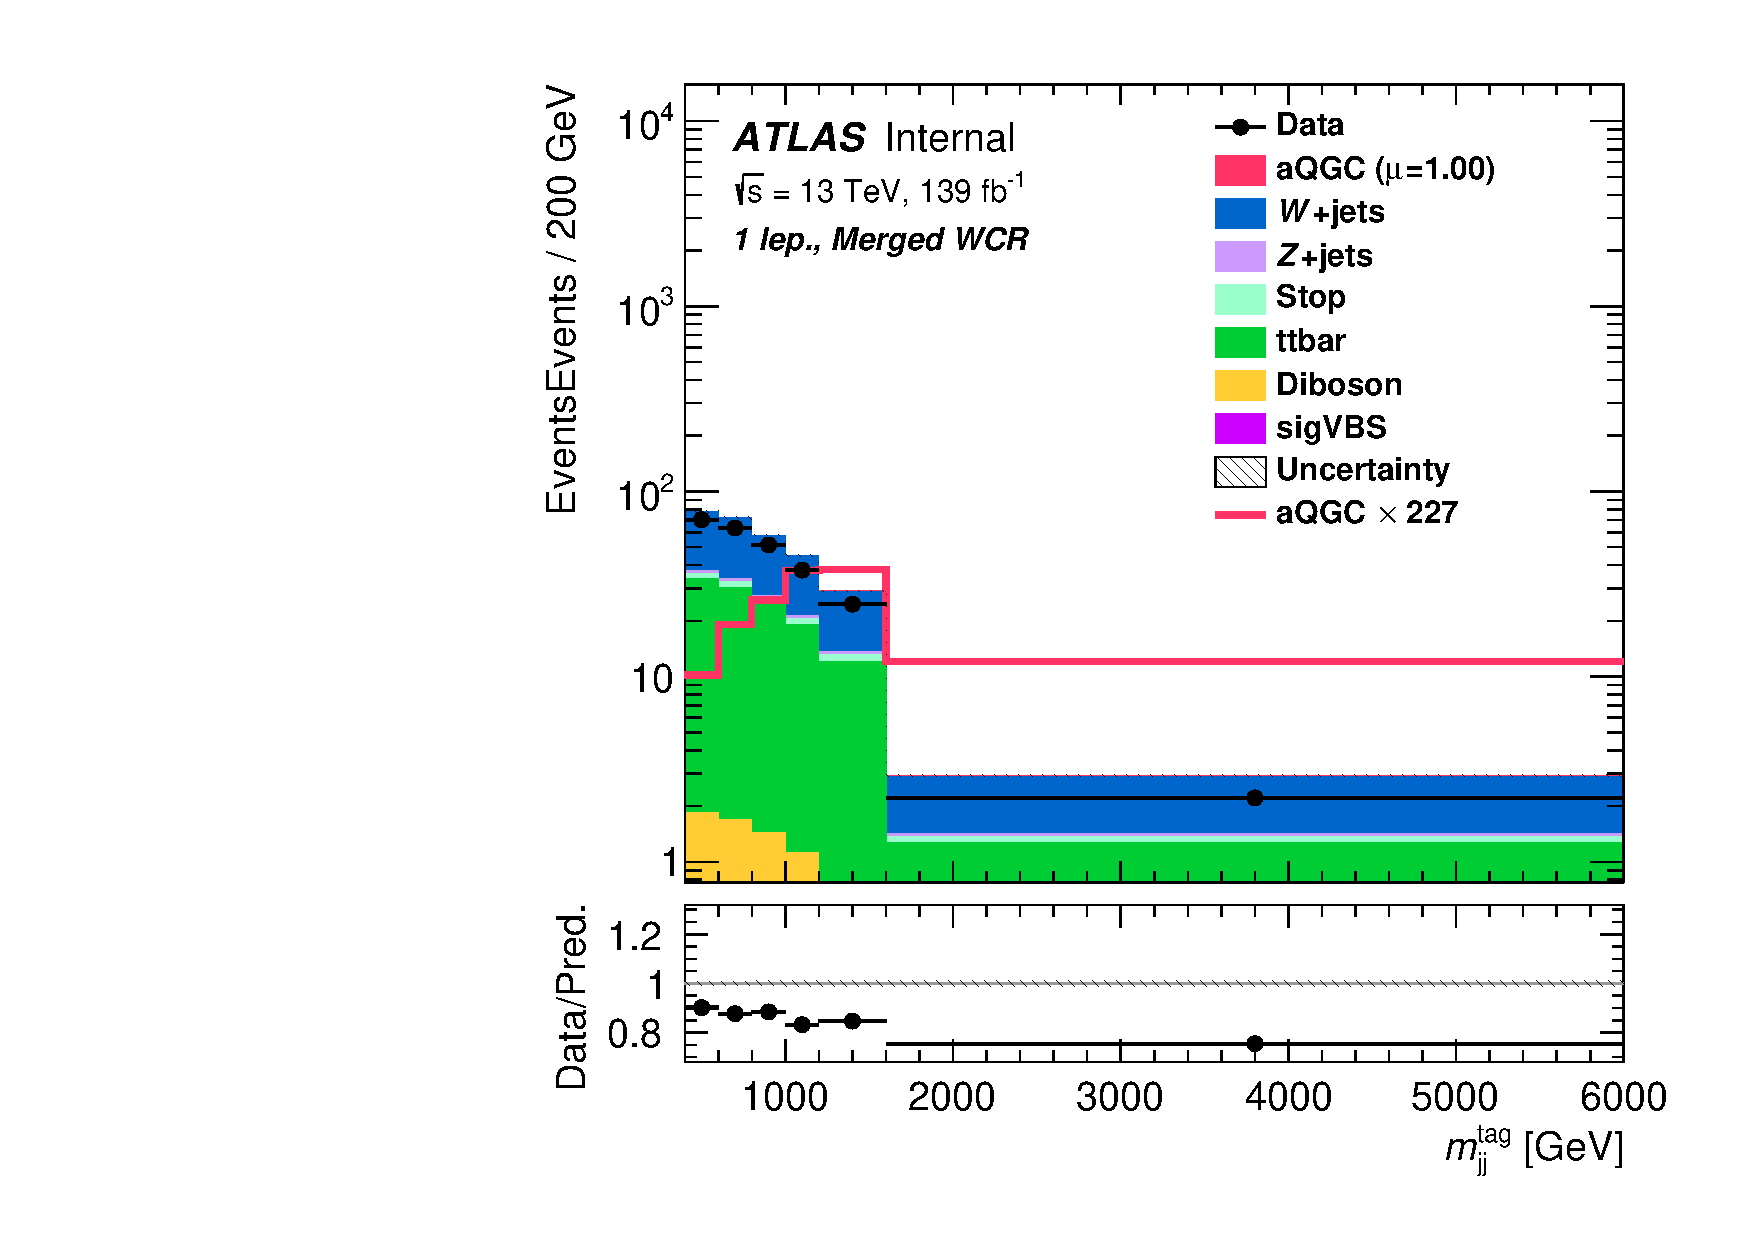
\includegraphics[width=0.32\textwidth]{figures/aQGC/Region_disttagMjj_DCRVjetMerged_BMin0_J0_incJet1_L1_T0_incFat1_Y6051_incTag1_Fat1_Prefitlog.pdf}}
    	\subfigure[ 1lep HP Top CR ]{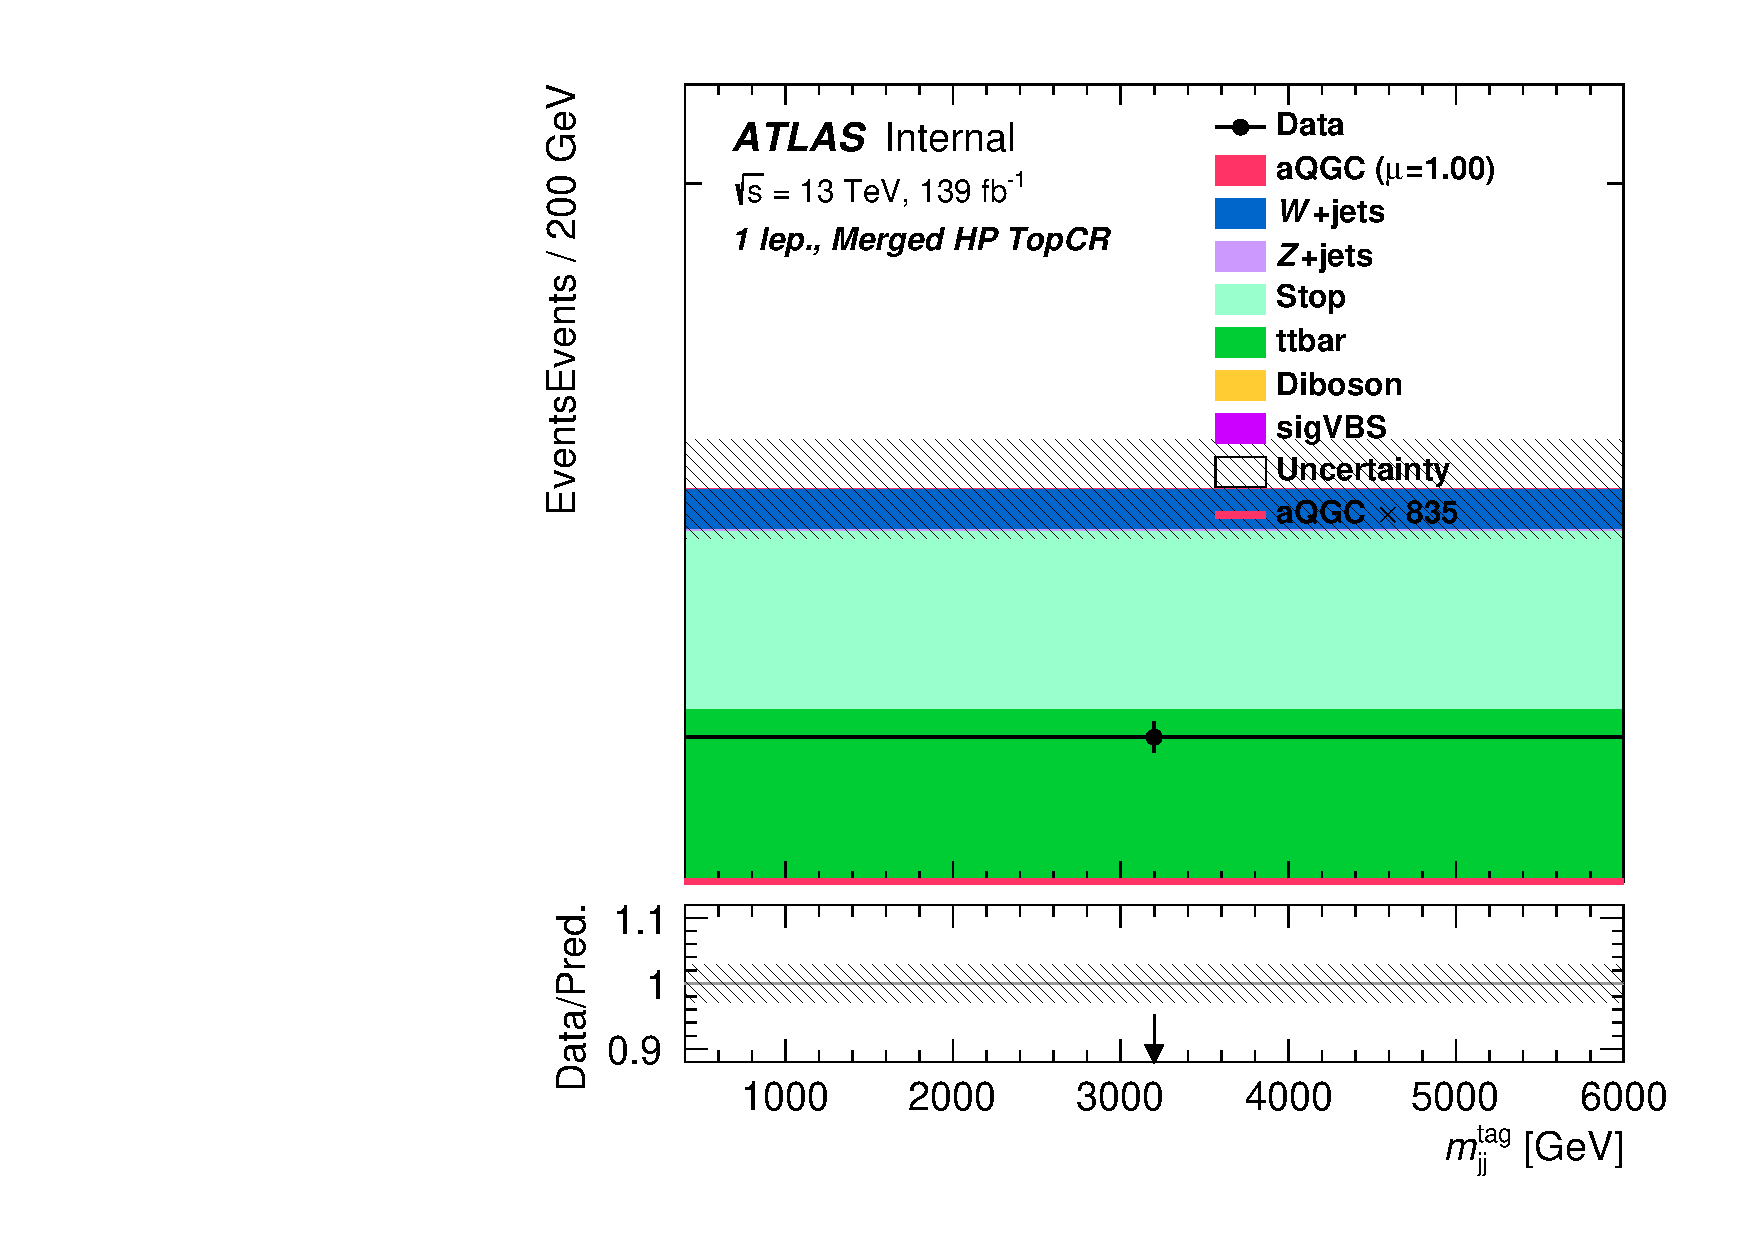
\includegraphics[width=0.32\textwidth]{figures/aQGC/Region_disttagMjj_DCRTopHP_BMin0_J0_incJet1_L1_T0_incFat1_Y6051_incTag1_Fat1_Prefitlog.pdf}}
    	\subfigure[ 1lep LP Top CR ]{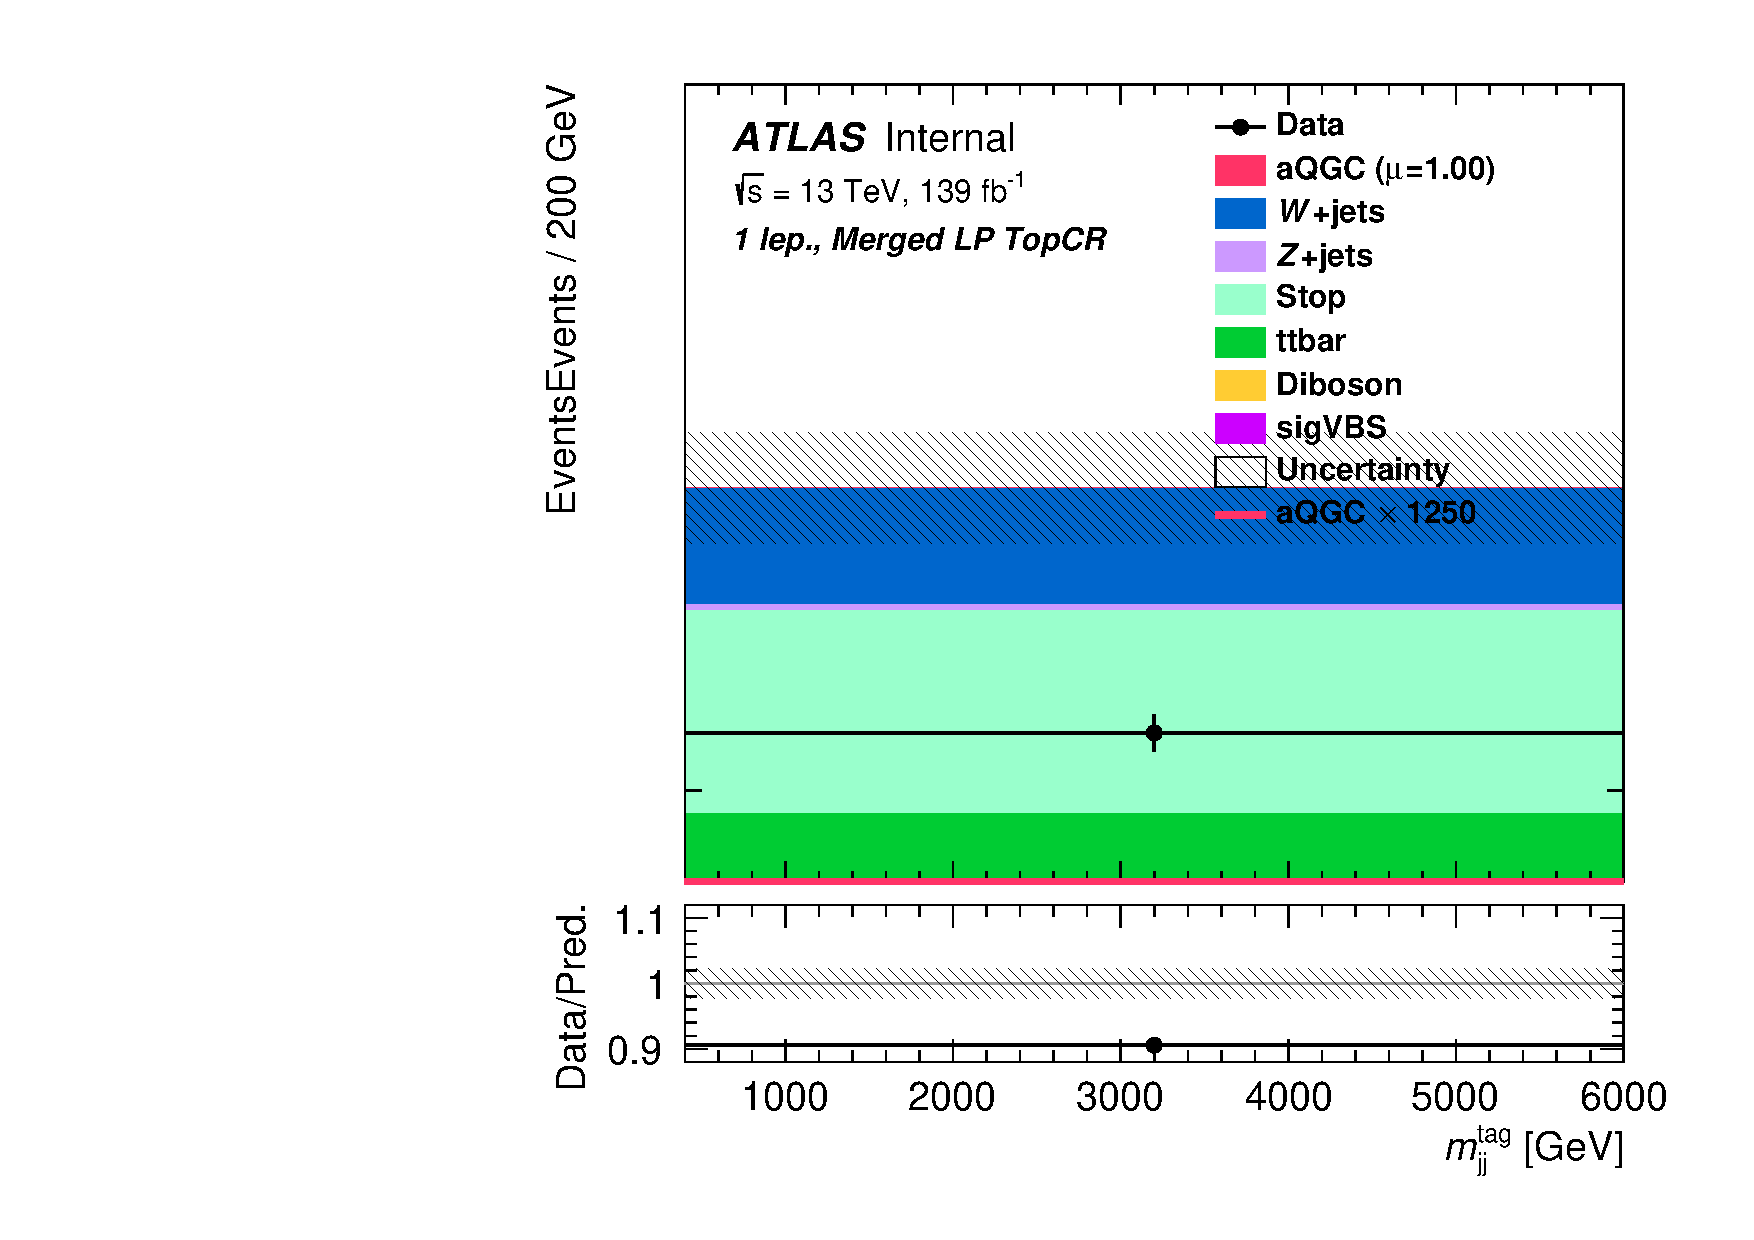
\includegraphics[width=0.32\textwidth]{figures/aQGC/Region_disttagMjj_DCRTopLP_BMin0_J0_incJet1_L1_T0_incFat1_Y6051_incTag1_Fat1_Prefitlog.pdf}}
    	\subfigure[ 1lep HP SR ]{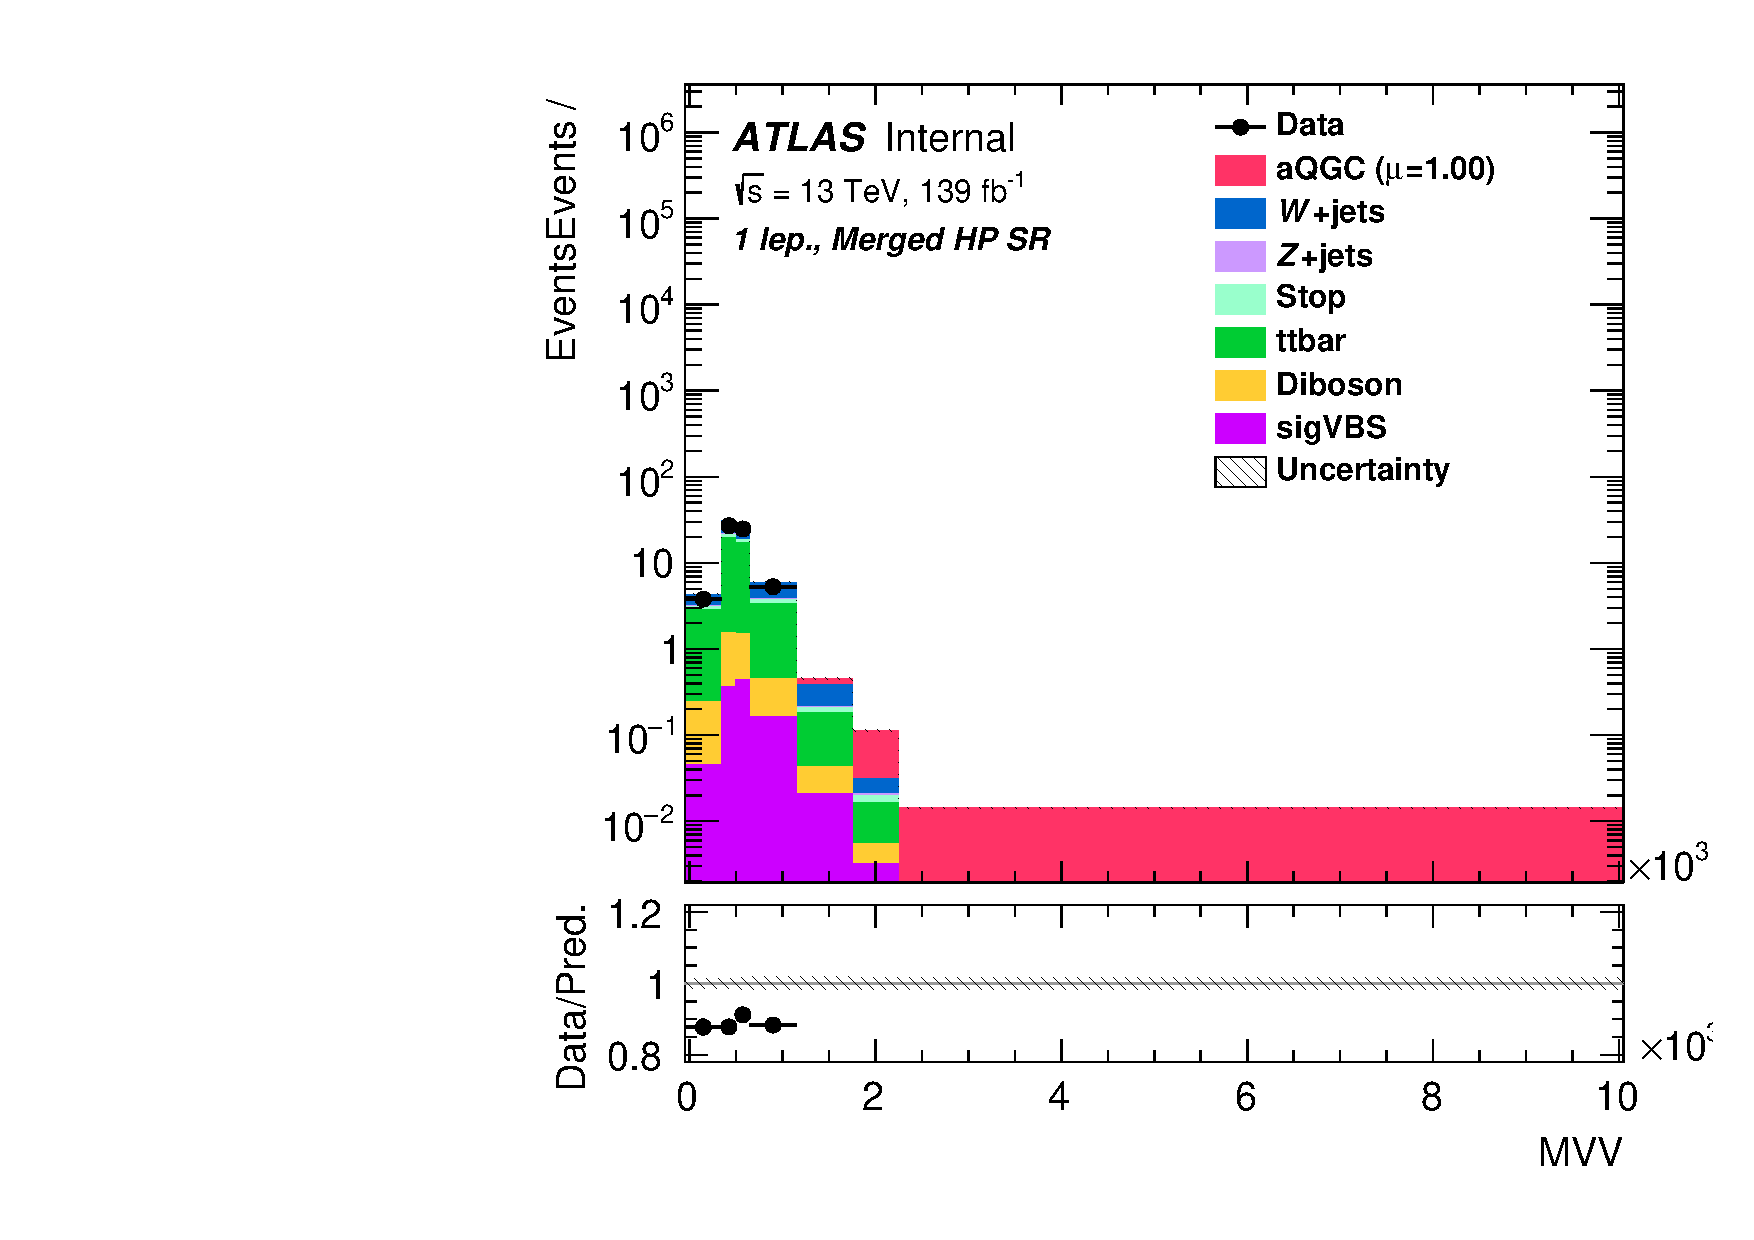
\includegraphics[width=0.32\textwidth]{figures/aQGC/Region_distMVV_DSRVBSHP_BMin0_J0_incJet1_L1_T0_incFat1_Y6051_incTag1_Fat1_Prefitlog.pdf}}
    	\subfigure[ 1lep LP SR ]{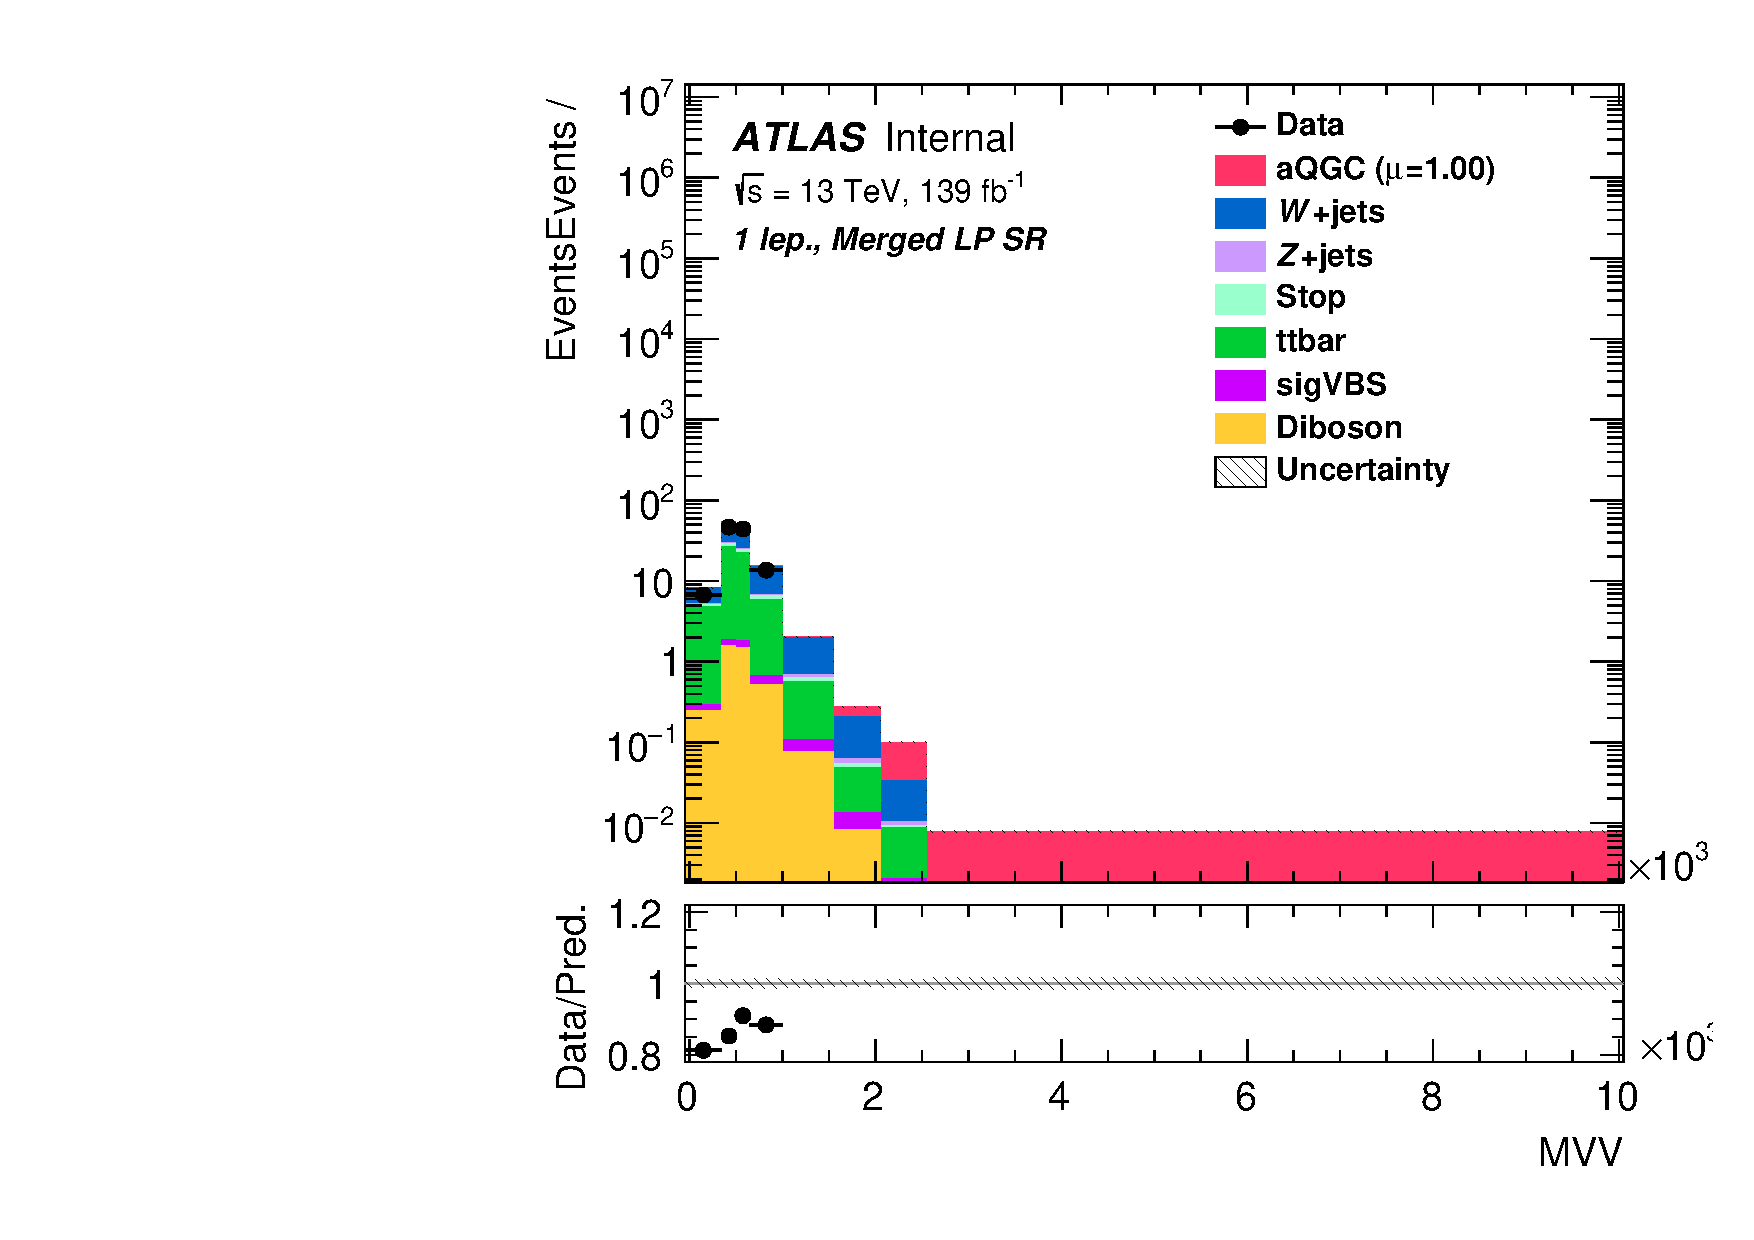
\includegraphics[width=0.32\textwidth]{figures/aQGC/Region_distMVV_DSRVBSLP_BMin0_J0_incJet1_L1_T0_incFat1_Y6051_incTag1_Fat1_Prefitlog.pdf}}
    	\subfigure[ 1lep resolved Vjet CR ]{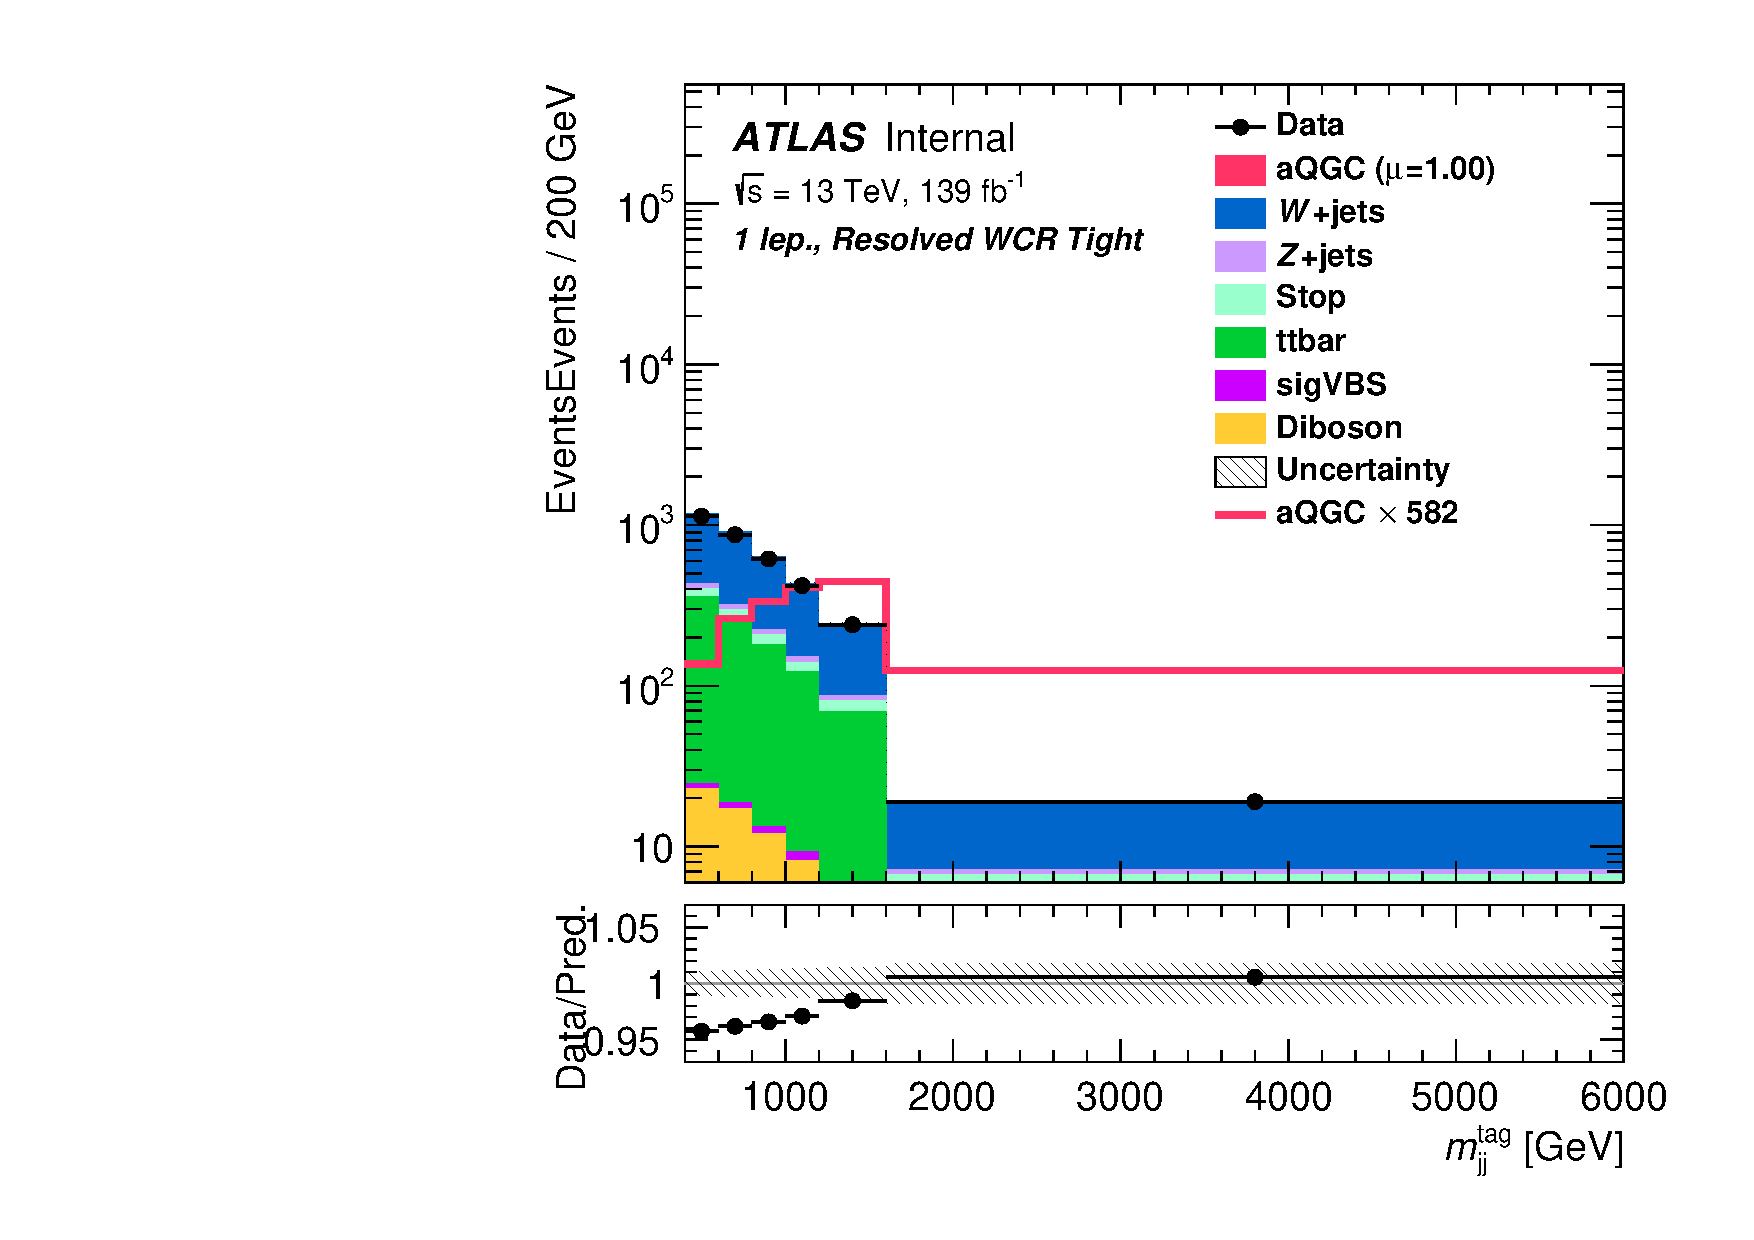
\includegraphics[width=0.32\textwidth]{figures/aQGC/Region_disttagMjj_DCRVjetTight_BMin0_T0_Y6051_incTag1_J2_L1_incJet1_Prefitlog.pdf}}
    	\subfigure[ 1lep resolved Top CR ]{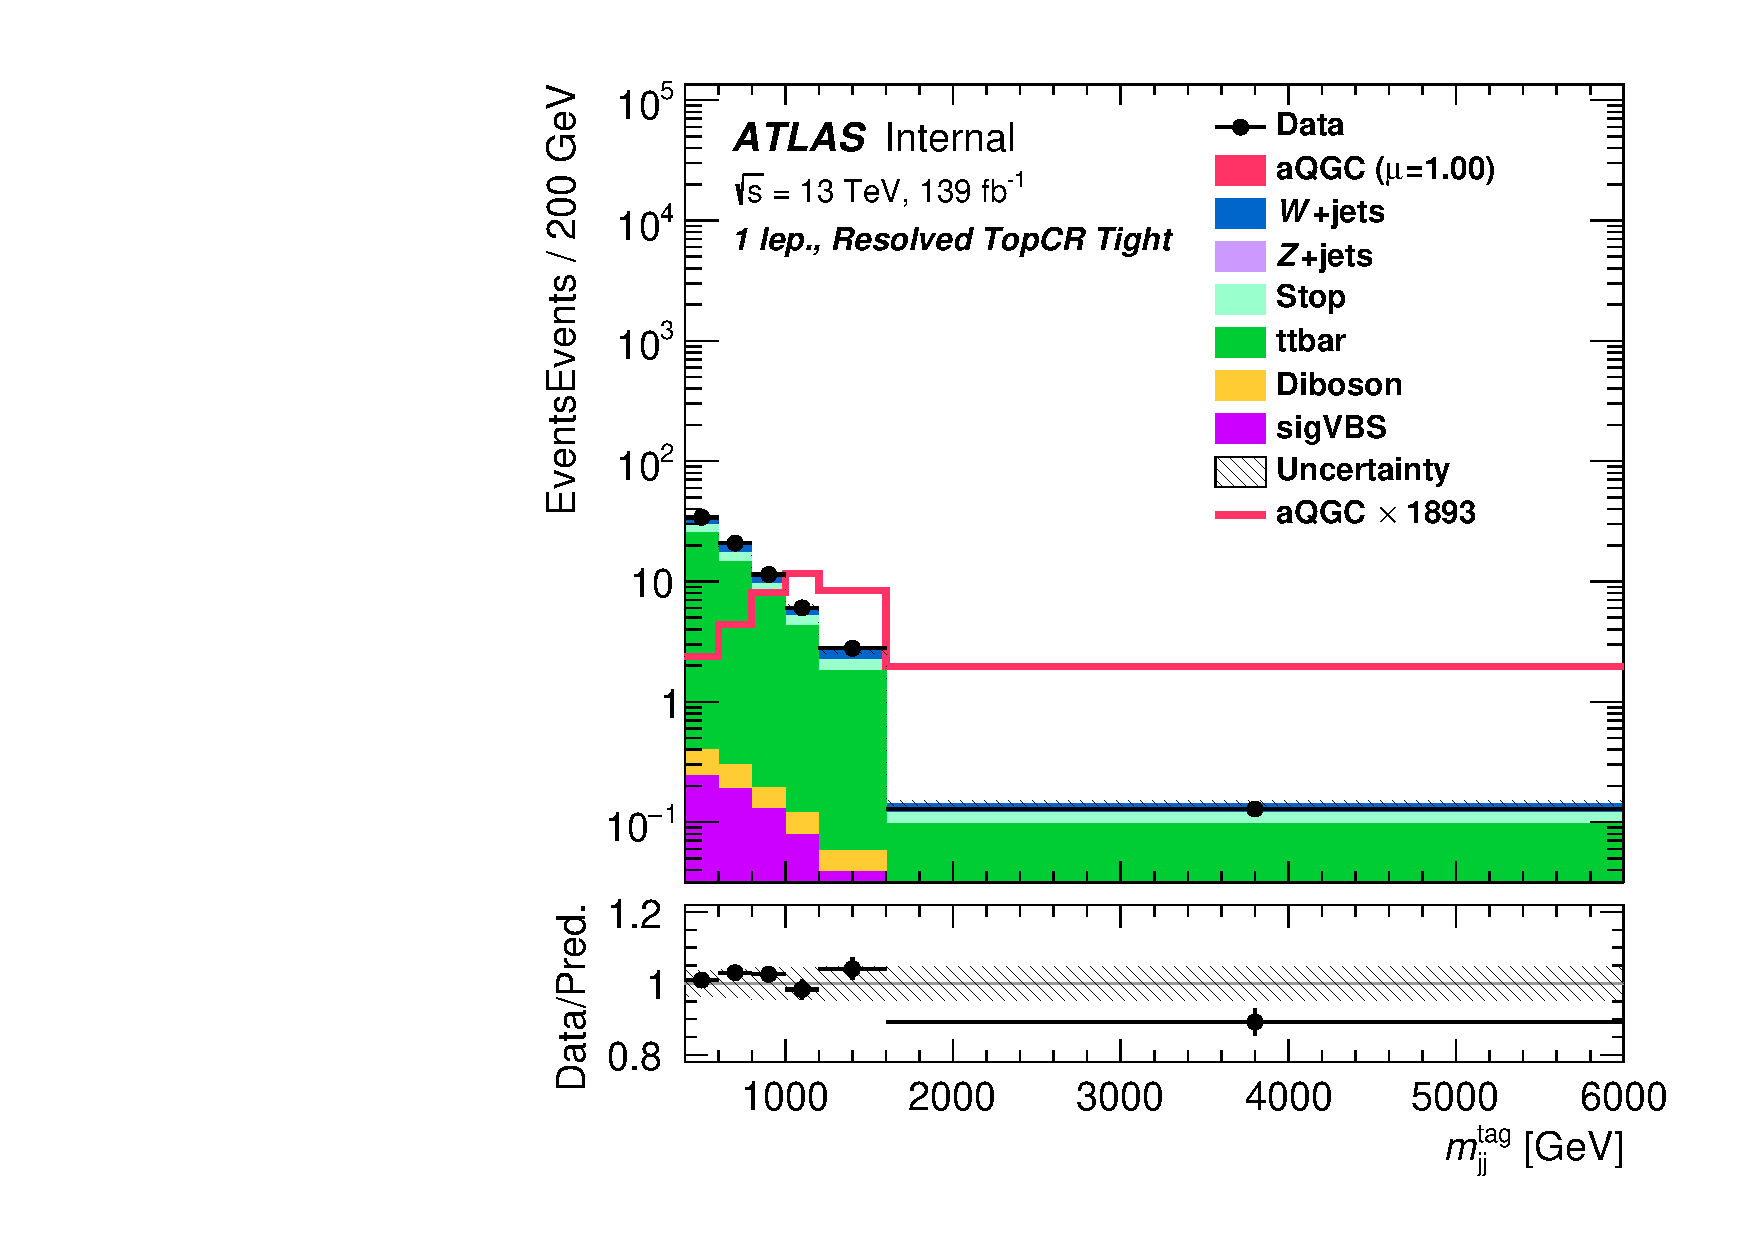
\includegraphics[width=0.32\textwidth]{figures/aQGC/Region_disttagMjj_DCRTopTight_BMin0_T0_Y6051_incTag1_J2_L1_incJet1_Prefitlog.pdf}}
    	\subfigure[ 1lep resolved SR ]{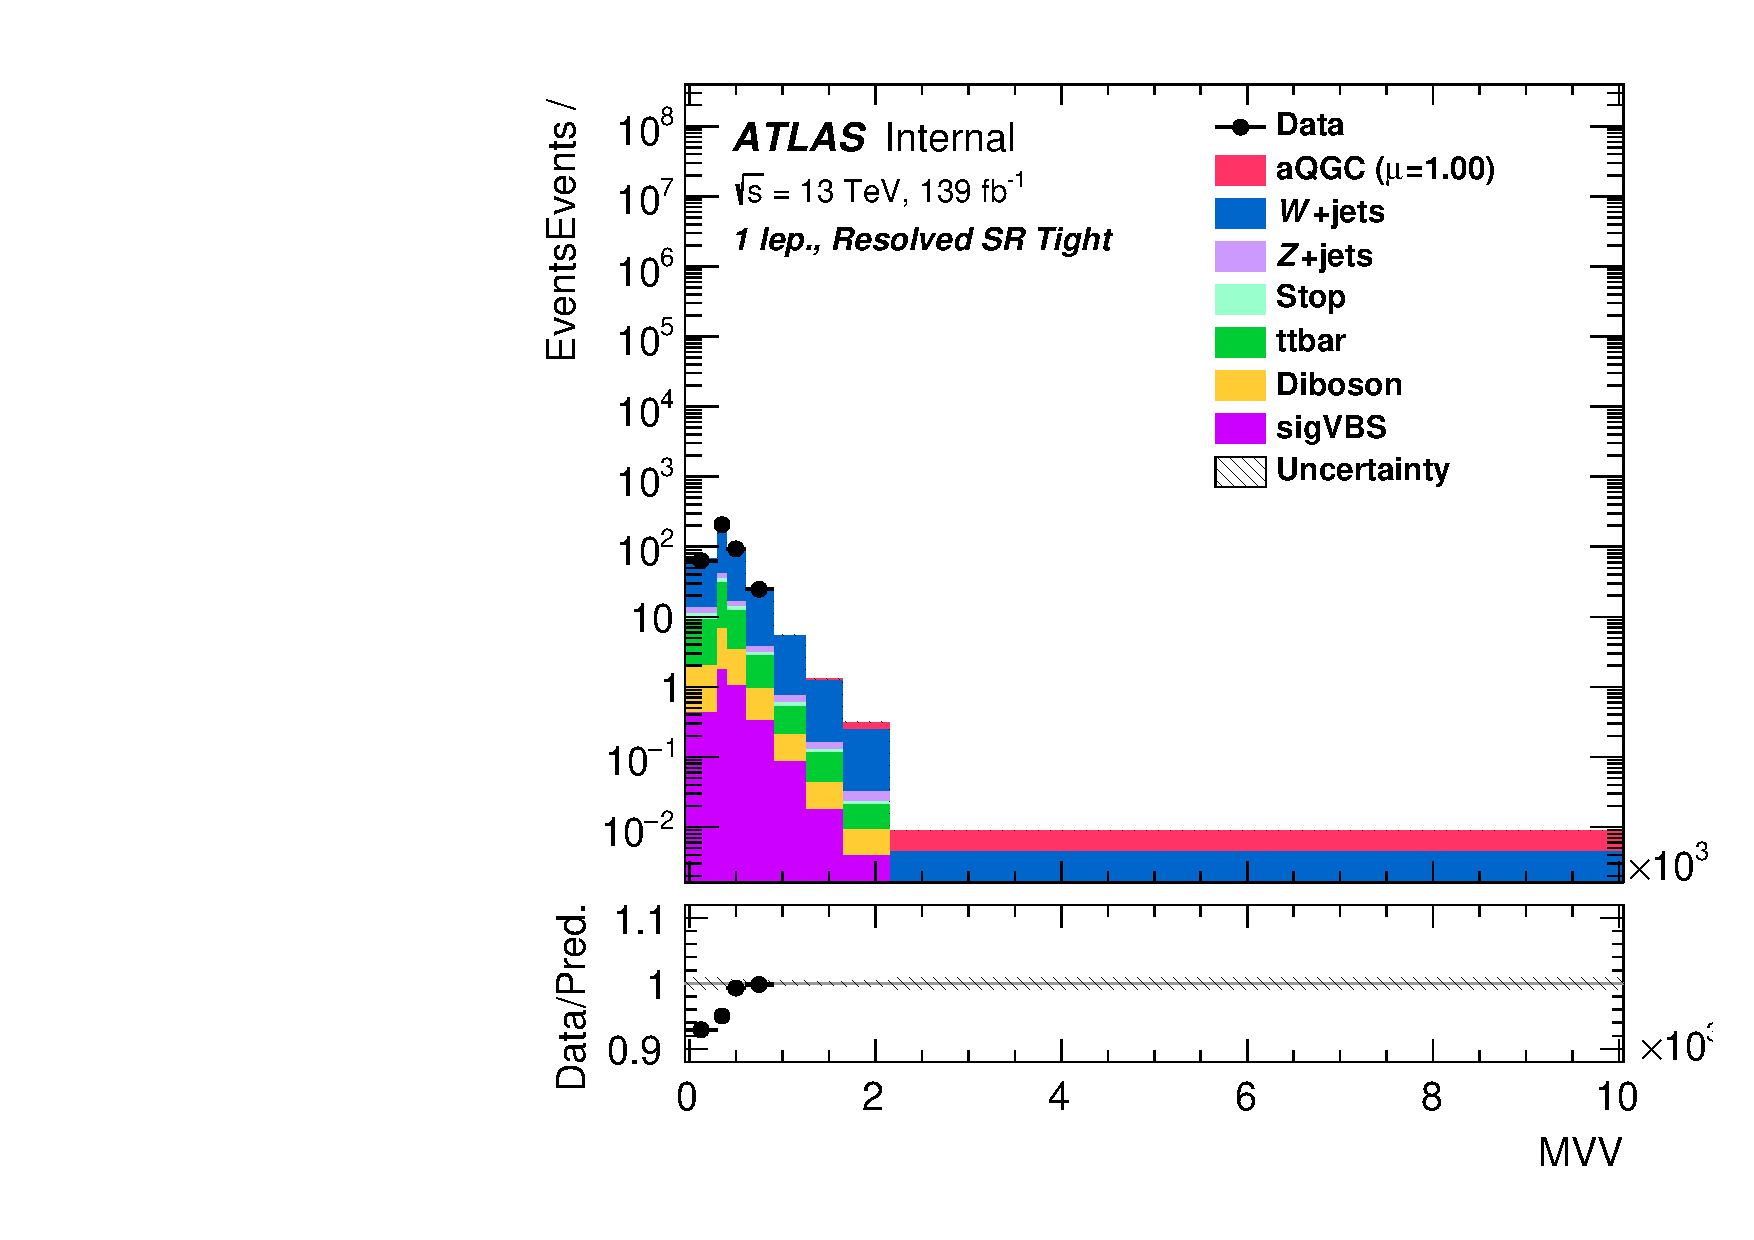
\includegraphics[width=0.32\textwidth]{figures/aQGC/Region_distMVV_DSRVBSTight_BMin0_T0_Y6051_incTag1_J2_L1_incJet1_Prefitlog.pdf}}
        \caption{Prefit plots for operator FT0 in \olep channel are shown. The standard model EW signal is floated as the background.}
        \label{fig:1lepFT0}
\end{figure}

\begin{figure}[ht]
    \centering
    	\subfigure[ 2lep merged CR ]{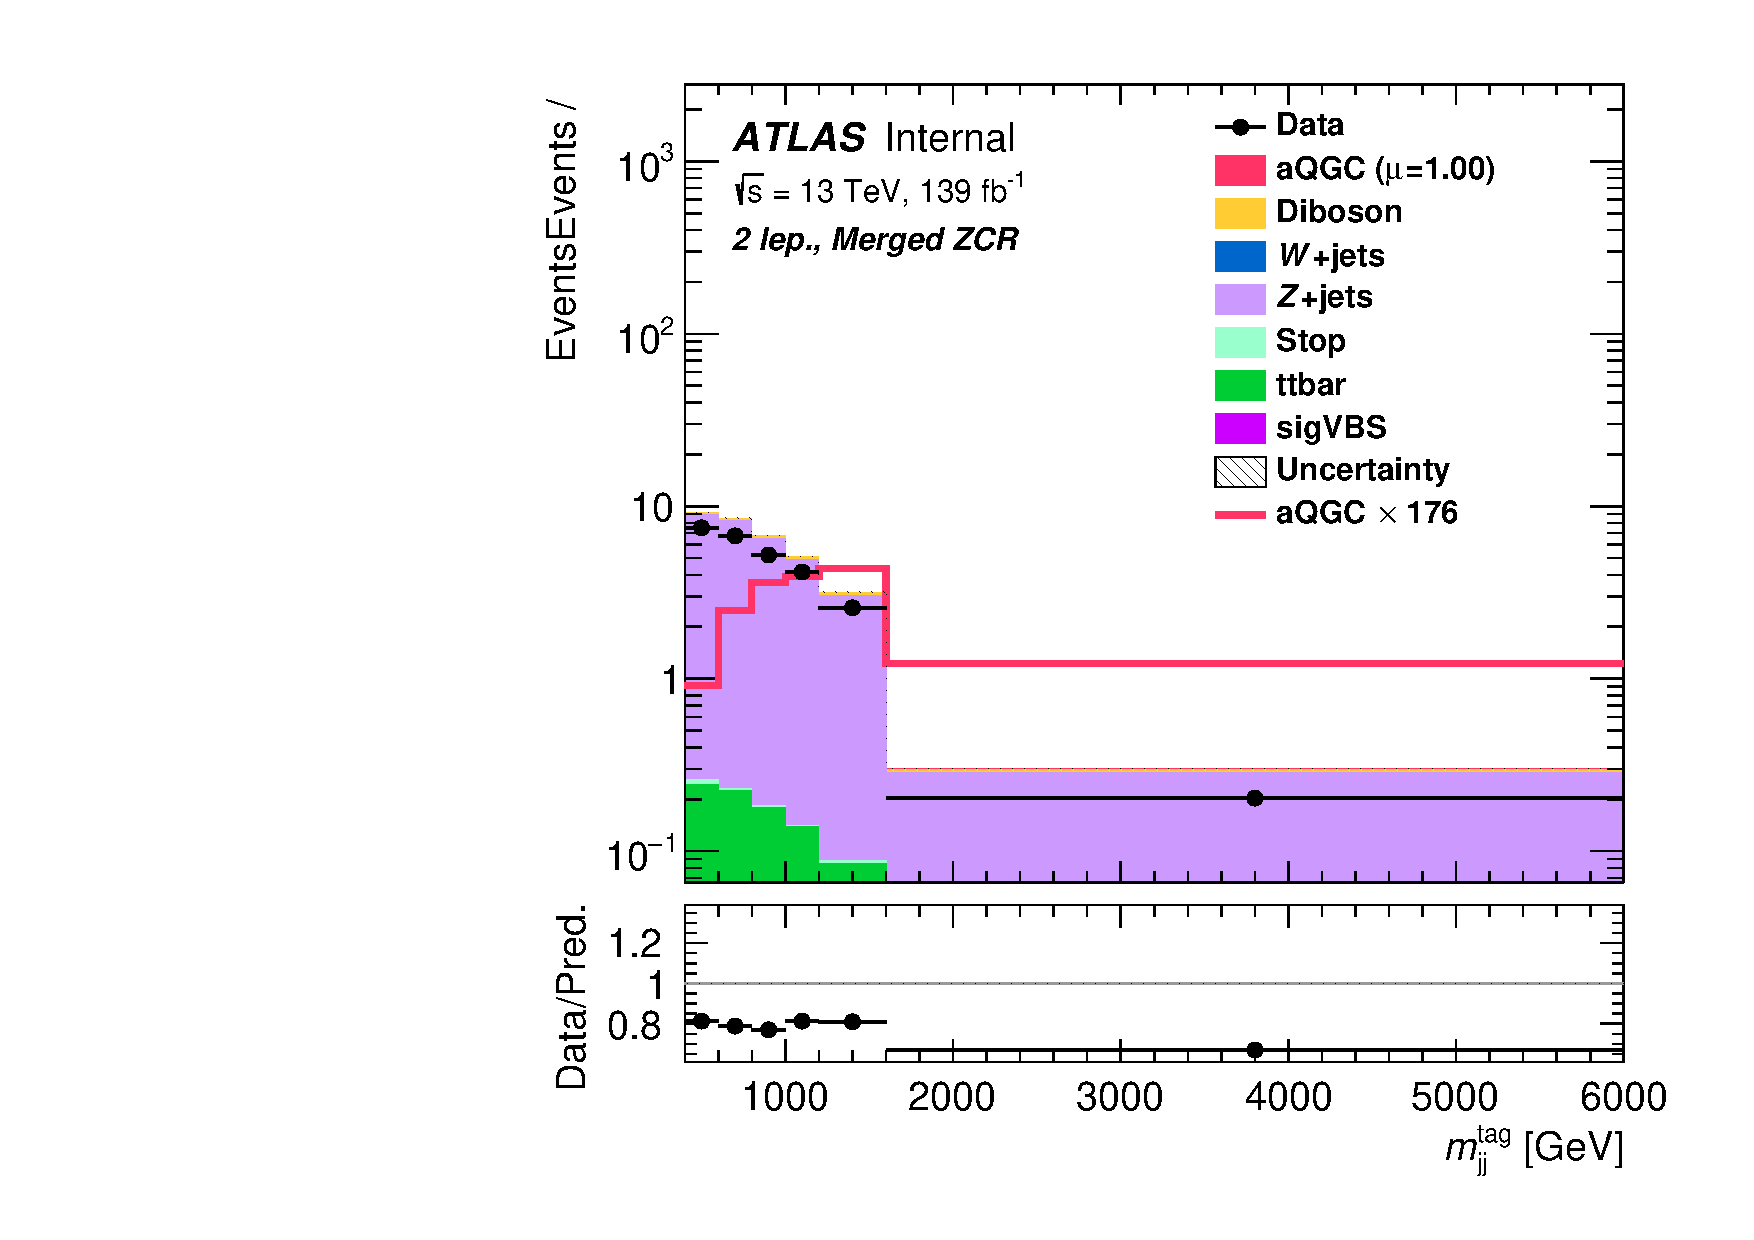
\includegraphics[width=0.32\textwidth]{figures/aQGC/Region_distMTagMerJets_DCRVjet_BMin0_J0_incJet1_L2_T0_incFat1_Y6051_incTag1_Fat1_Prefitlog.pdf}}
    	\subfigure[ 2lep HP SR ]{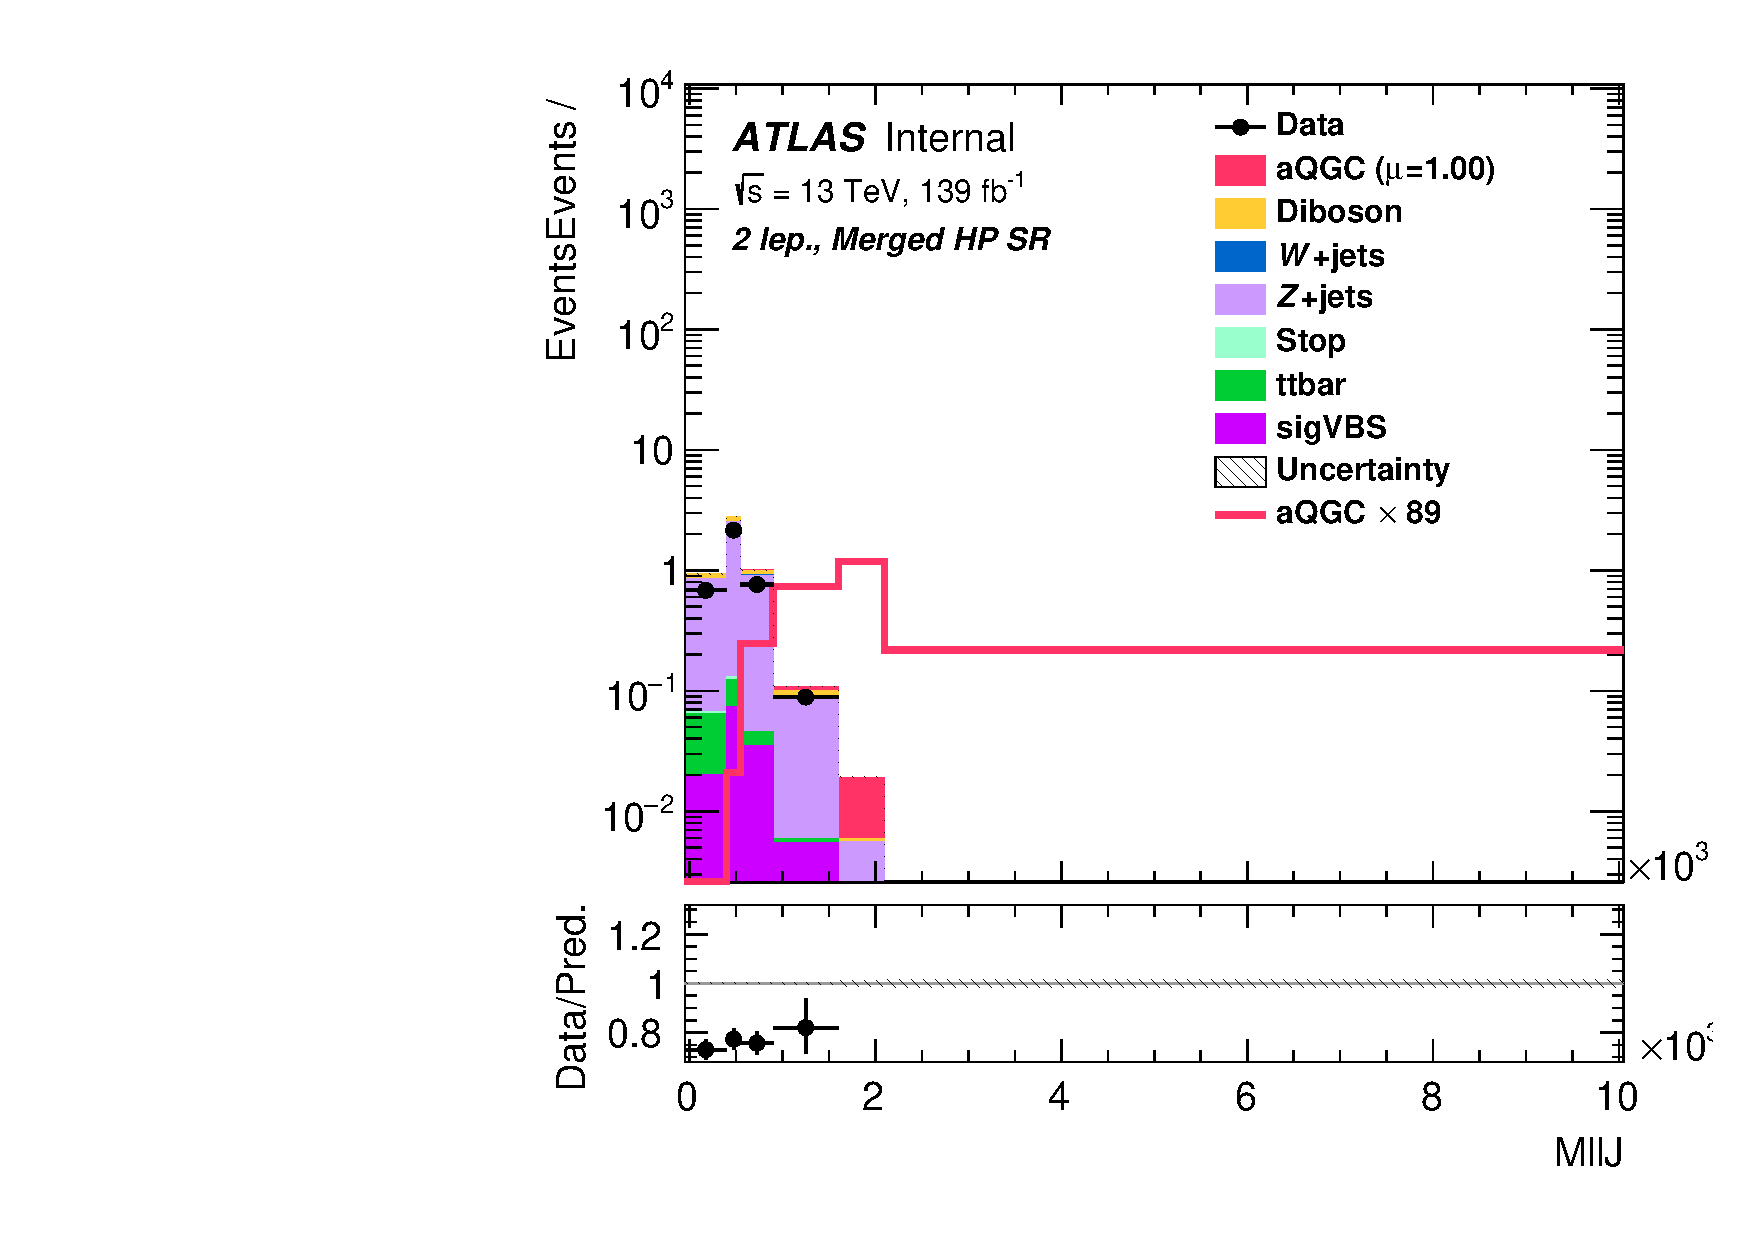
\includegraphics[width=0.32\textwidth]{figures/aQGC/Region_distMllJ_DSRVBSHP_BMin0_J0_incJet1_L2_T0_incFat1_Y6051_incTag1_Fat1_Prefitlog.pdf}}
    	\subfigure[ 2lep LP SR ]{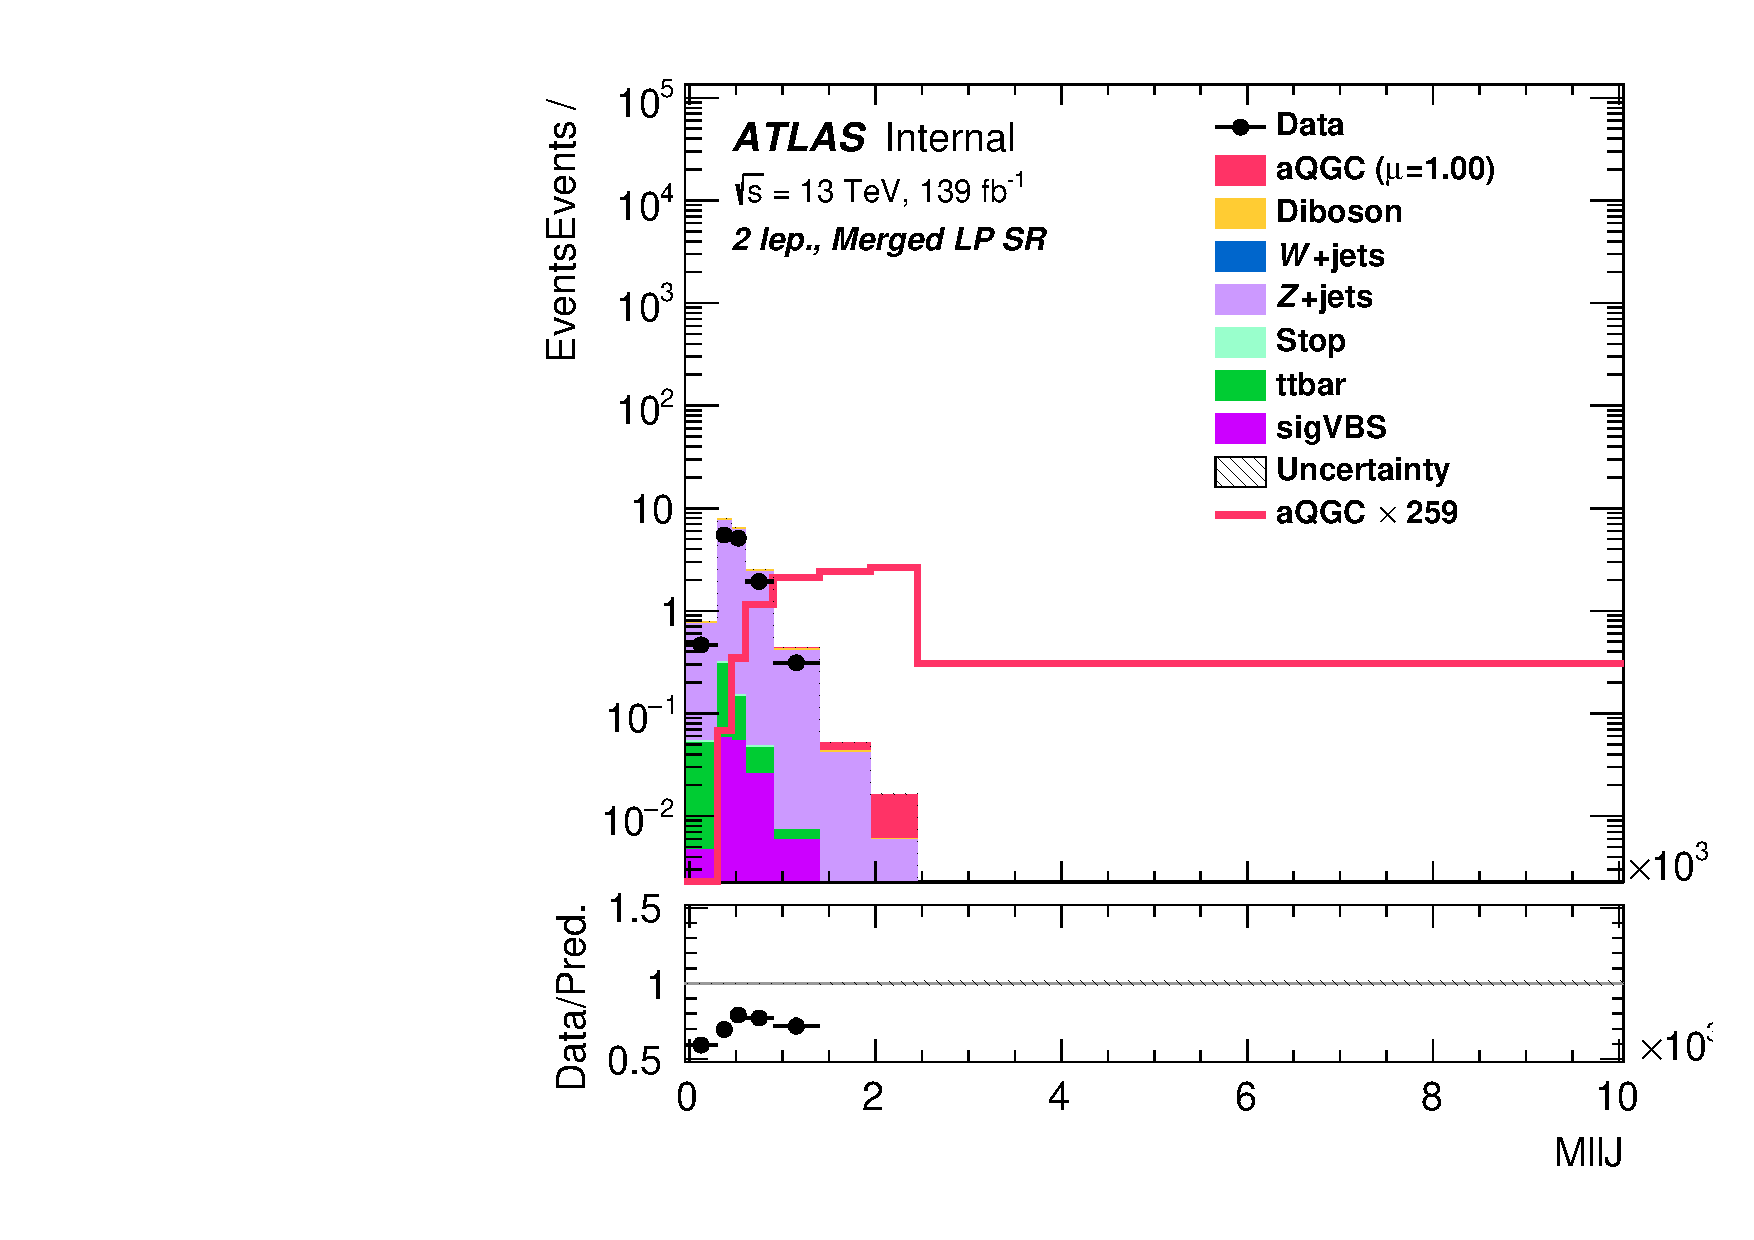
\includegraphics[width=0.32\textwidth]{figures/aQGC/Region_distMllJ_DSRVBSLP_BMin0_J0_incJet1_L2_T0_incFat1_Y6051_incTag1_Fat1_Prefitlog.pdf}}
    	\subfigure[ 2lep resolved CR ]{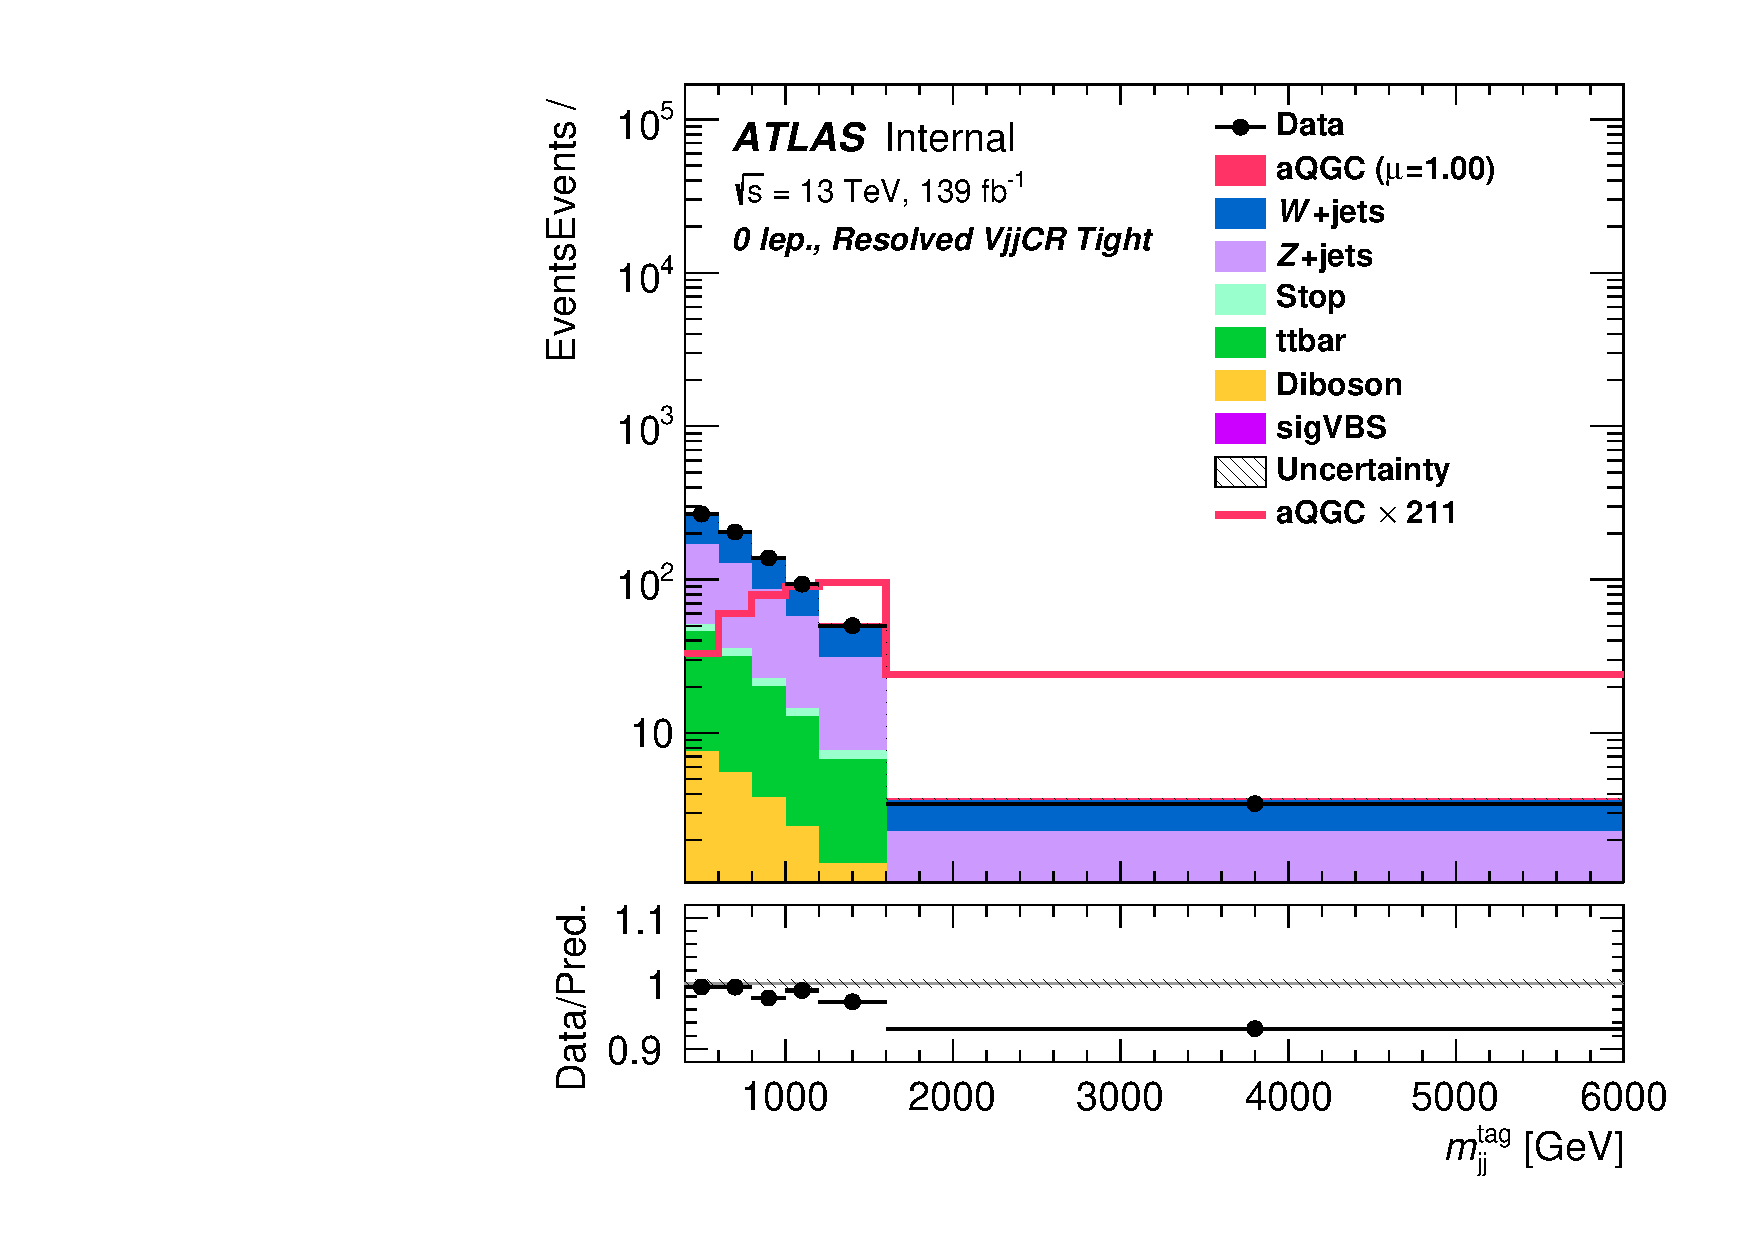
\includegraphics[width=0.32\textwidth]{figures/aQGC/Region_distMTagJets_DCRVjetFid_BMin0_T0_Y6051_incTag1_J2_L0_incJet1_Prefitlog.pdf}}
    	\subfigure[ 2lep resolved SR ]{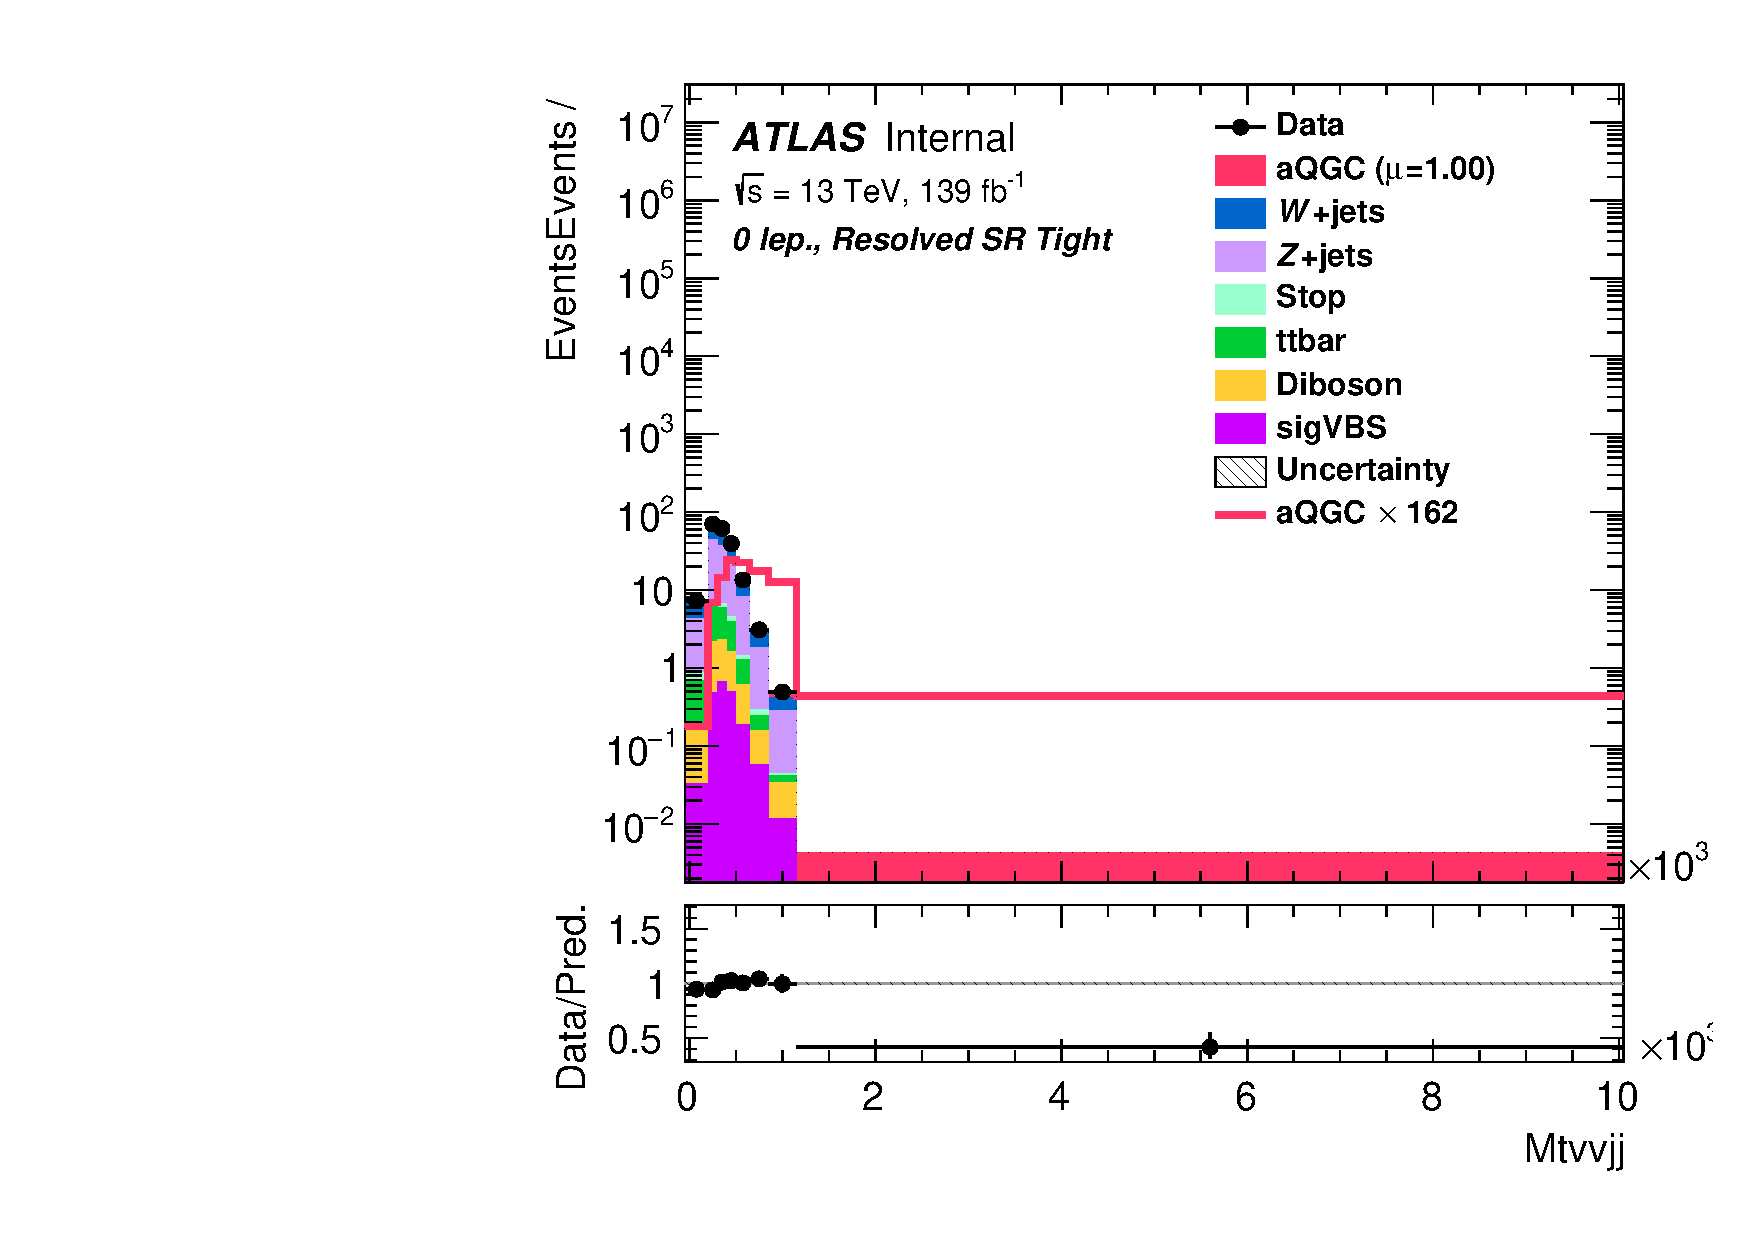
\includegraphics[width=0.32\textwidth]{figures/aQGC/Region_distMtvvjj_DSRVBSFid_BMin0_T0_Y6051_incTag1_J2_L0_incJet1_Prefitlog.pdf}}
        \caption{Prefit plots for operator FT0 in \tlep channel are shown. The standard model EW signal is floated as the background.}
        \label{fig:2lepFT0}
\end{figure}

\subsection{2-bin $m_{VV}$ approach}
\label{subsec:2binapproach}

There is a problem when we use the $m_{VV}$ distribution in the fit.
The normalization of the SM electroweak signal cannot be determined, since its shape is similar to the other background processes, as shown in Figure~\ref{fig:2lepaQGCshapeMVV}.
%RNN score shows the separation between standard model and the background, so the 2D fit of $m_{VV}$ and RNN score can be useful since we can use both separation powers. Spliting $m_{VV}$ in 2-bin is studied as the minimum case of 2D fit.

Unconditional asimov fit for FT0 signal in only \tlep channel is performed and compared in two options :
\begin{itemize}
  \item Fit $m_{VV}$ distribution as discriminant, as shown in section~\ref{subsec:aqgc_limit}
  \item Split the $m_{VV}$ into 2 bins ;  \\
        LowMVV : $m_{VV}$ $< 2000$~GeV \\
        HighMVV : $m_{VV}$ $\geq 2000$~GeV \\
        then fit simultaneously with RNN score as discriminant
\end{itemize}
Prefit plots are shown in figure~\ref{fig:2lepTwoBin} in the second option.
The expected limits and uncertainty of the expected signal strength of FT0 signal are shown in table~\ref{tab:2binlimit}.

\begin{figure}[ht]
    \centering
    	\subfigure[ 2lep merged CR ]{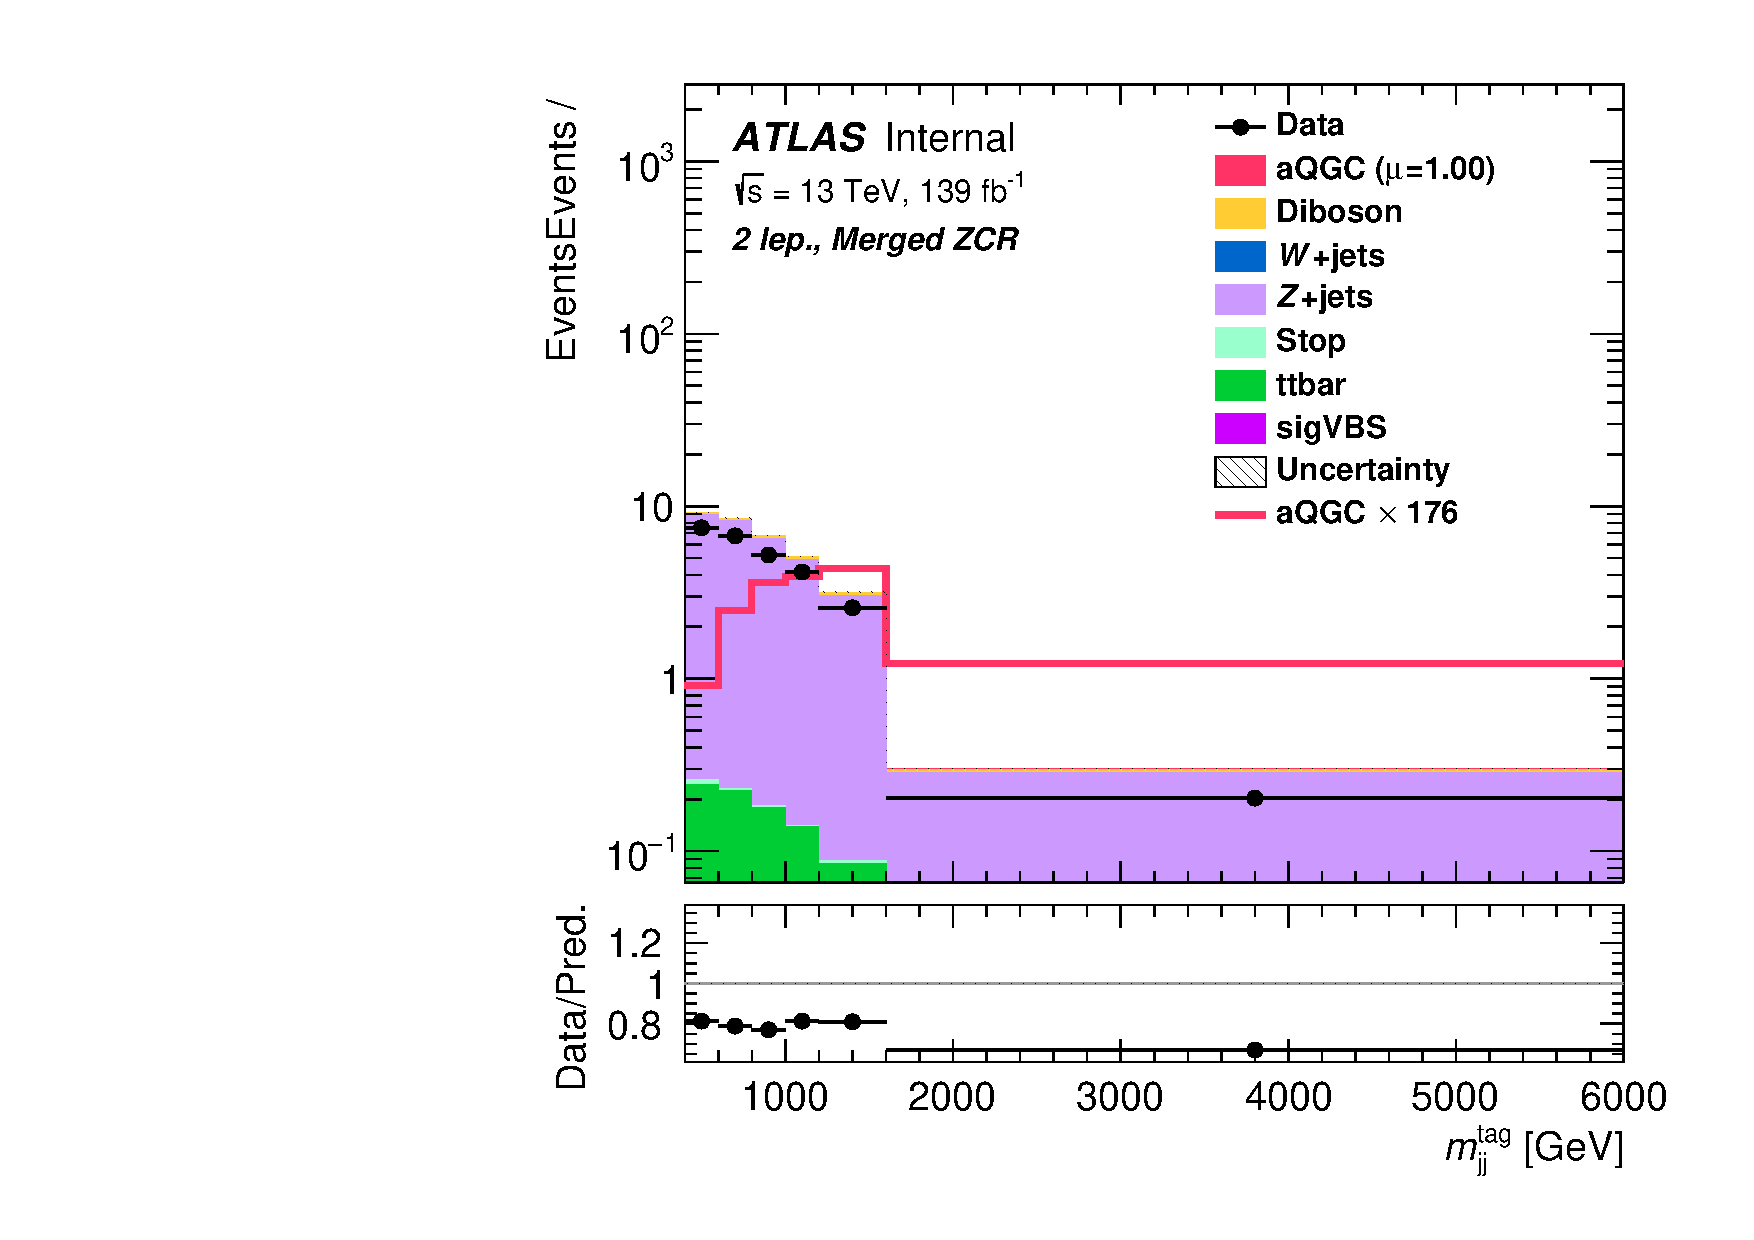
\includegraphics[width=0.32\textwidth]{figures/aQGC/Region_distMTagMerJets_DCRVjet_BMin0_J0_incJet1_L2_T0_incFat1_Y6051_incTag1_Fat1_Prefitlog.pdf}}
    	\subfigure[ 2lep HP LowMVV SR ]{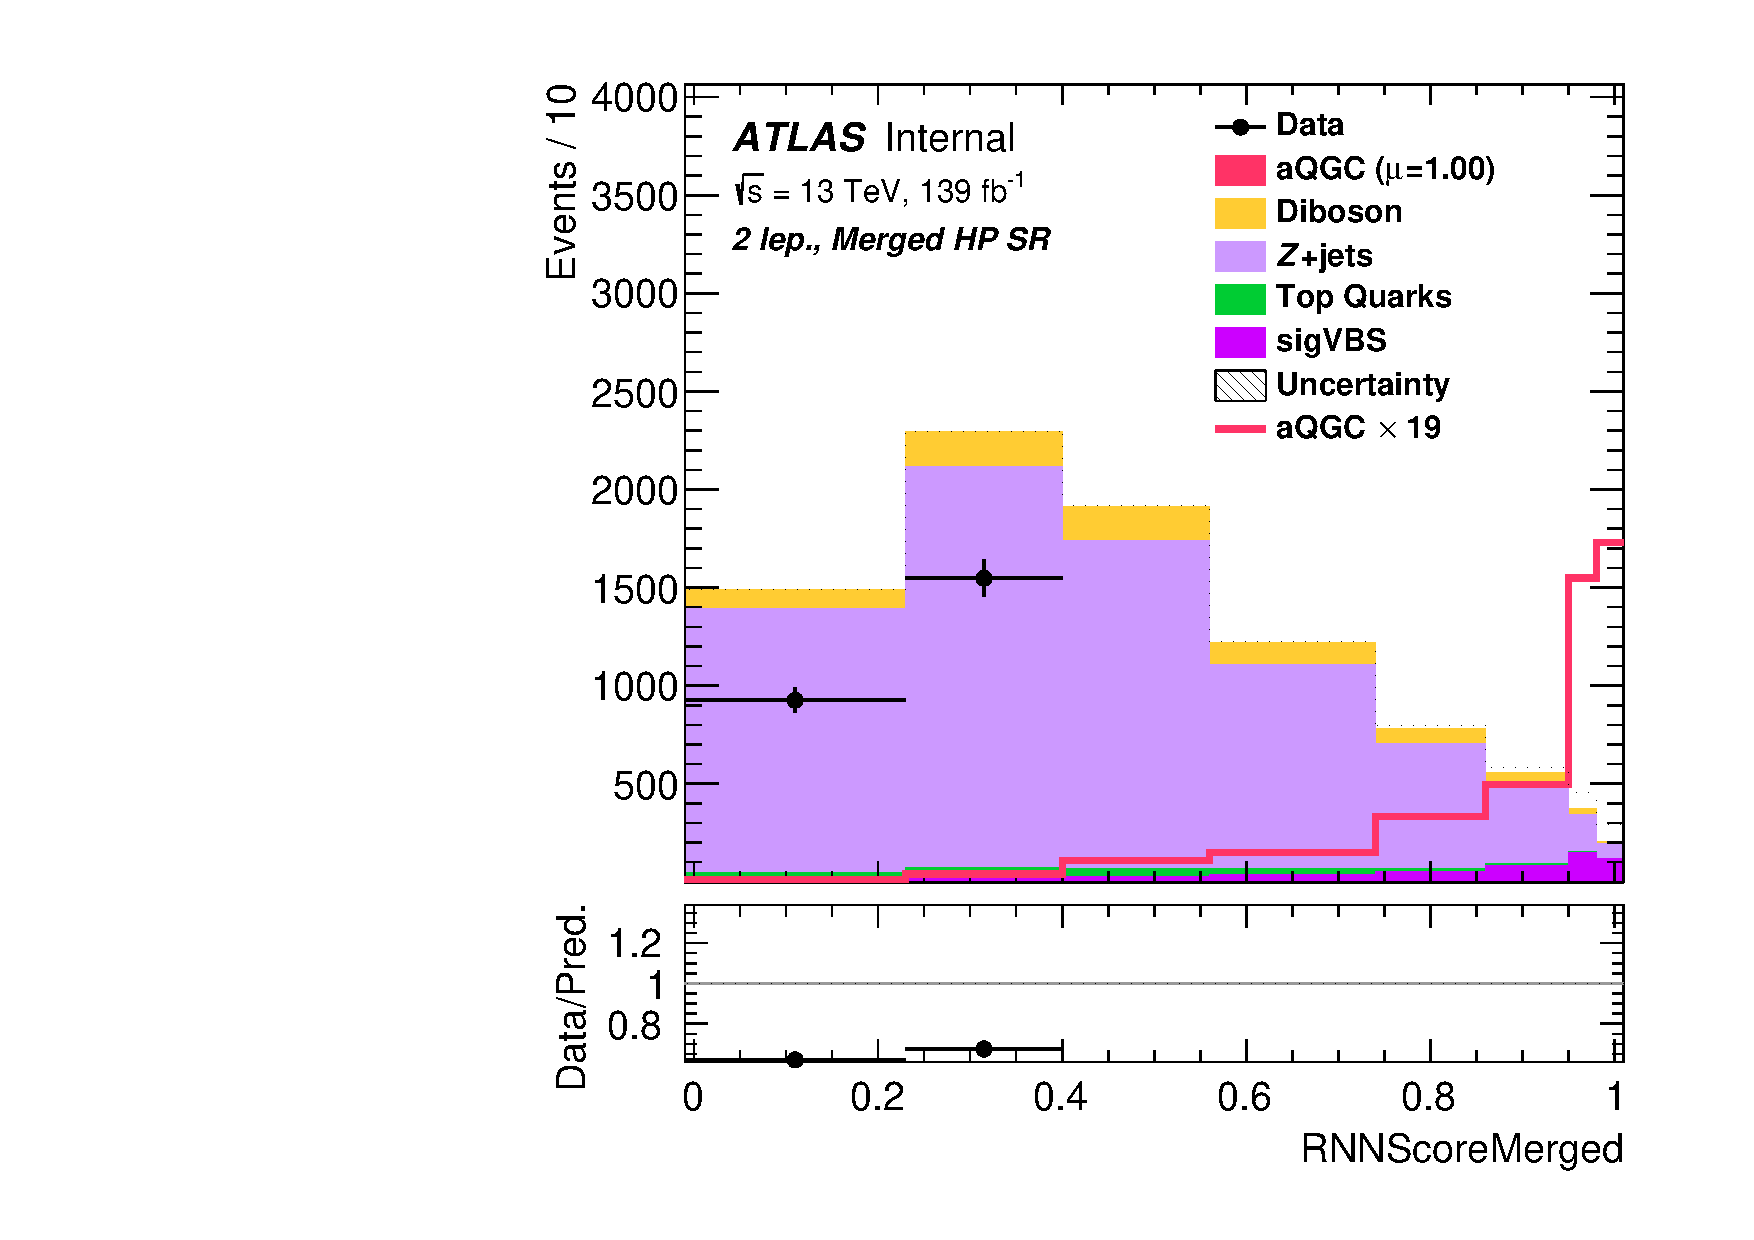
\includegraphics[width=0.32\textwidth]{figures/aQGC/Region_distRNNScoreMerged_DSRVBSHPLMVV_BMin0_J0_incJet1_L2_T0_incFat1_Y6051_incTag1_Fat1_Prefit.pdf}}
    	\subfigure[ 2lep HP HighMVV SR ]{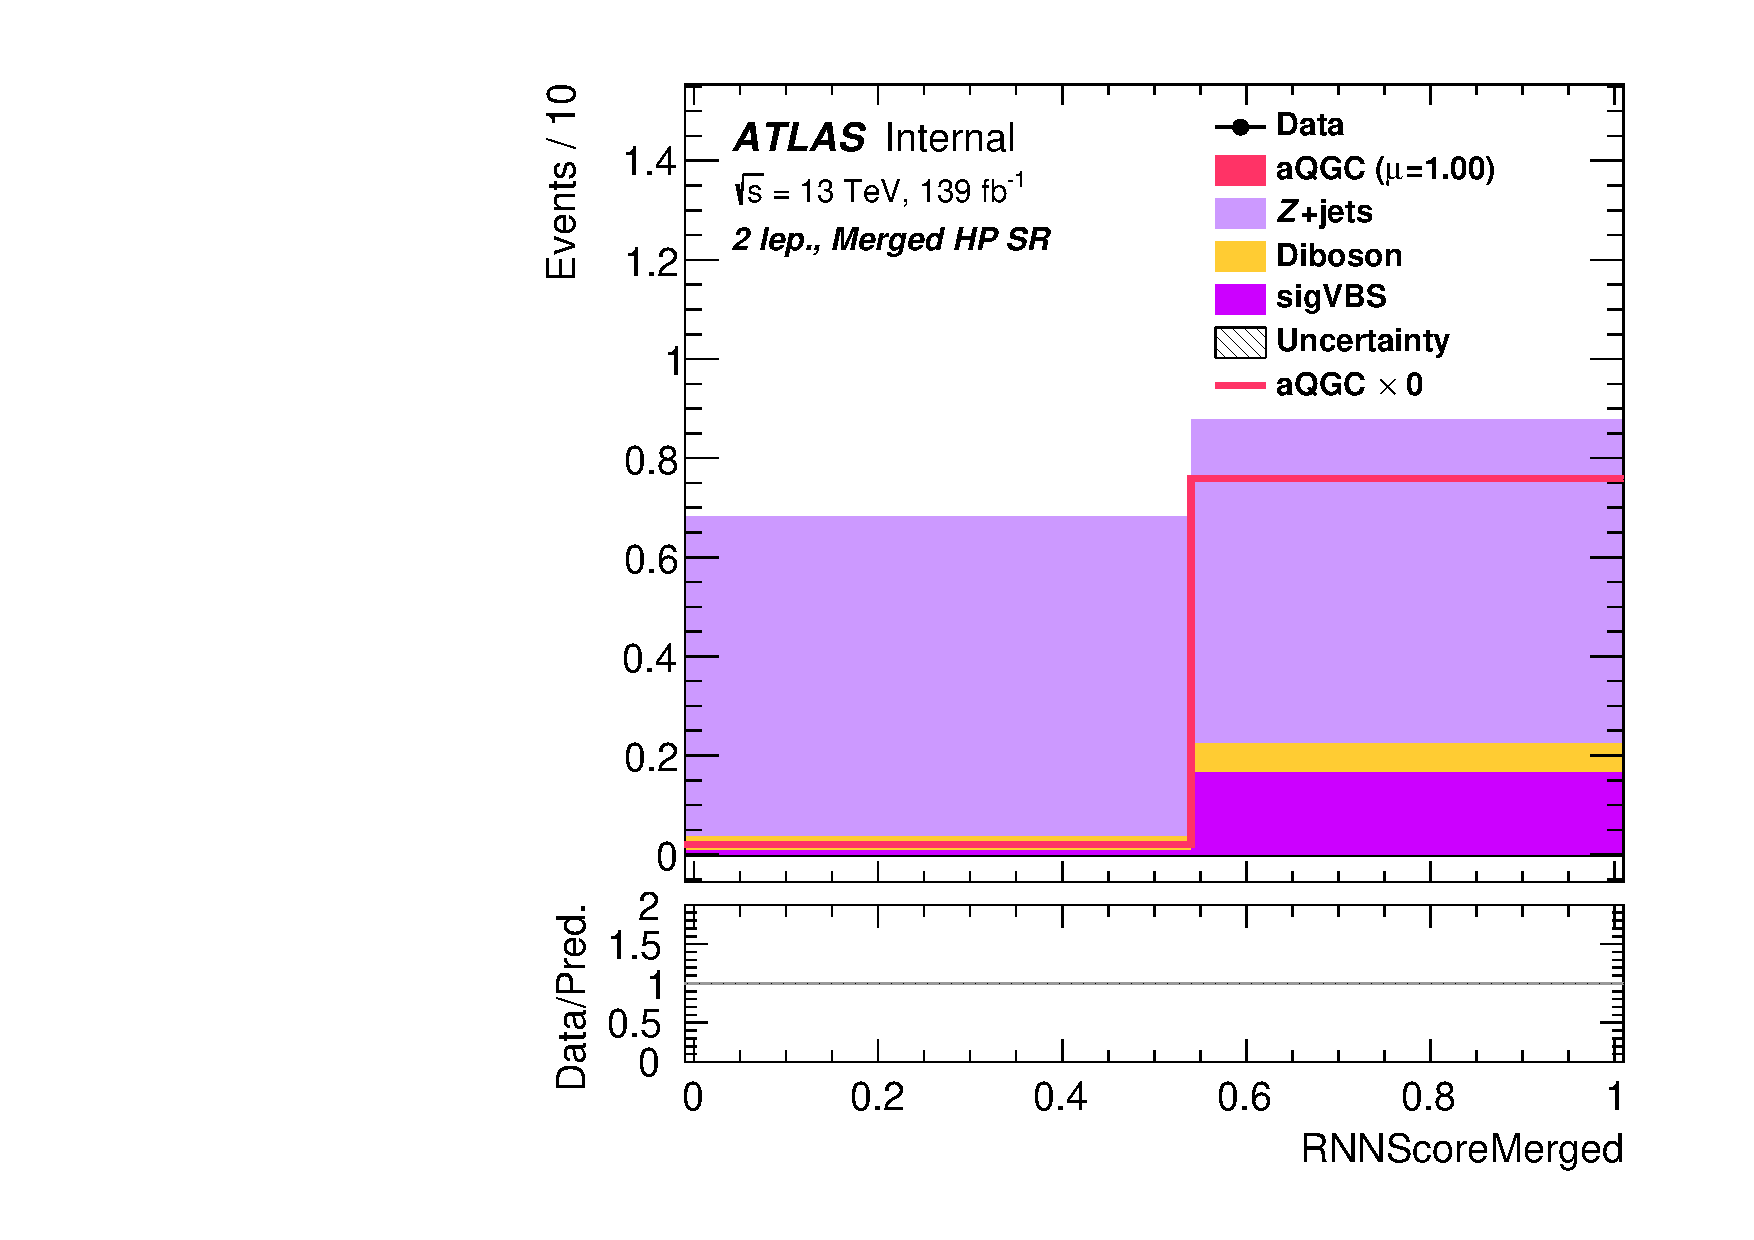
\includegraphics[width=0.32\textwidth]{figures/aQGC/Region_distRNNScoreMerged_DSRVBSHPHMVV_BMin0_J0_incJet1_L2_T0_incFat1_Y6051_incTag1_Fat1_Prefit.pdf}}
    	\subfigure[ 2lep LP LowMVV SR ]{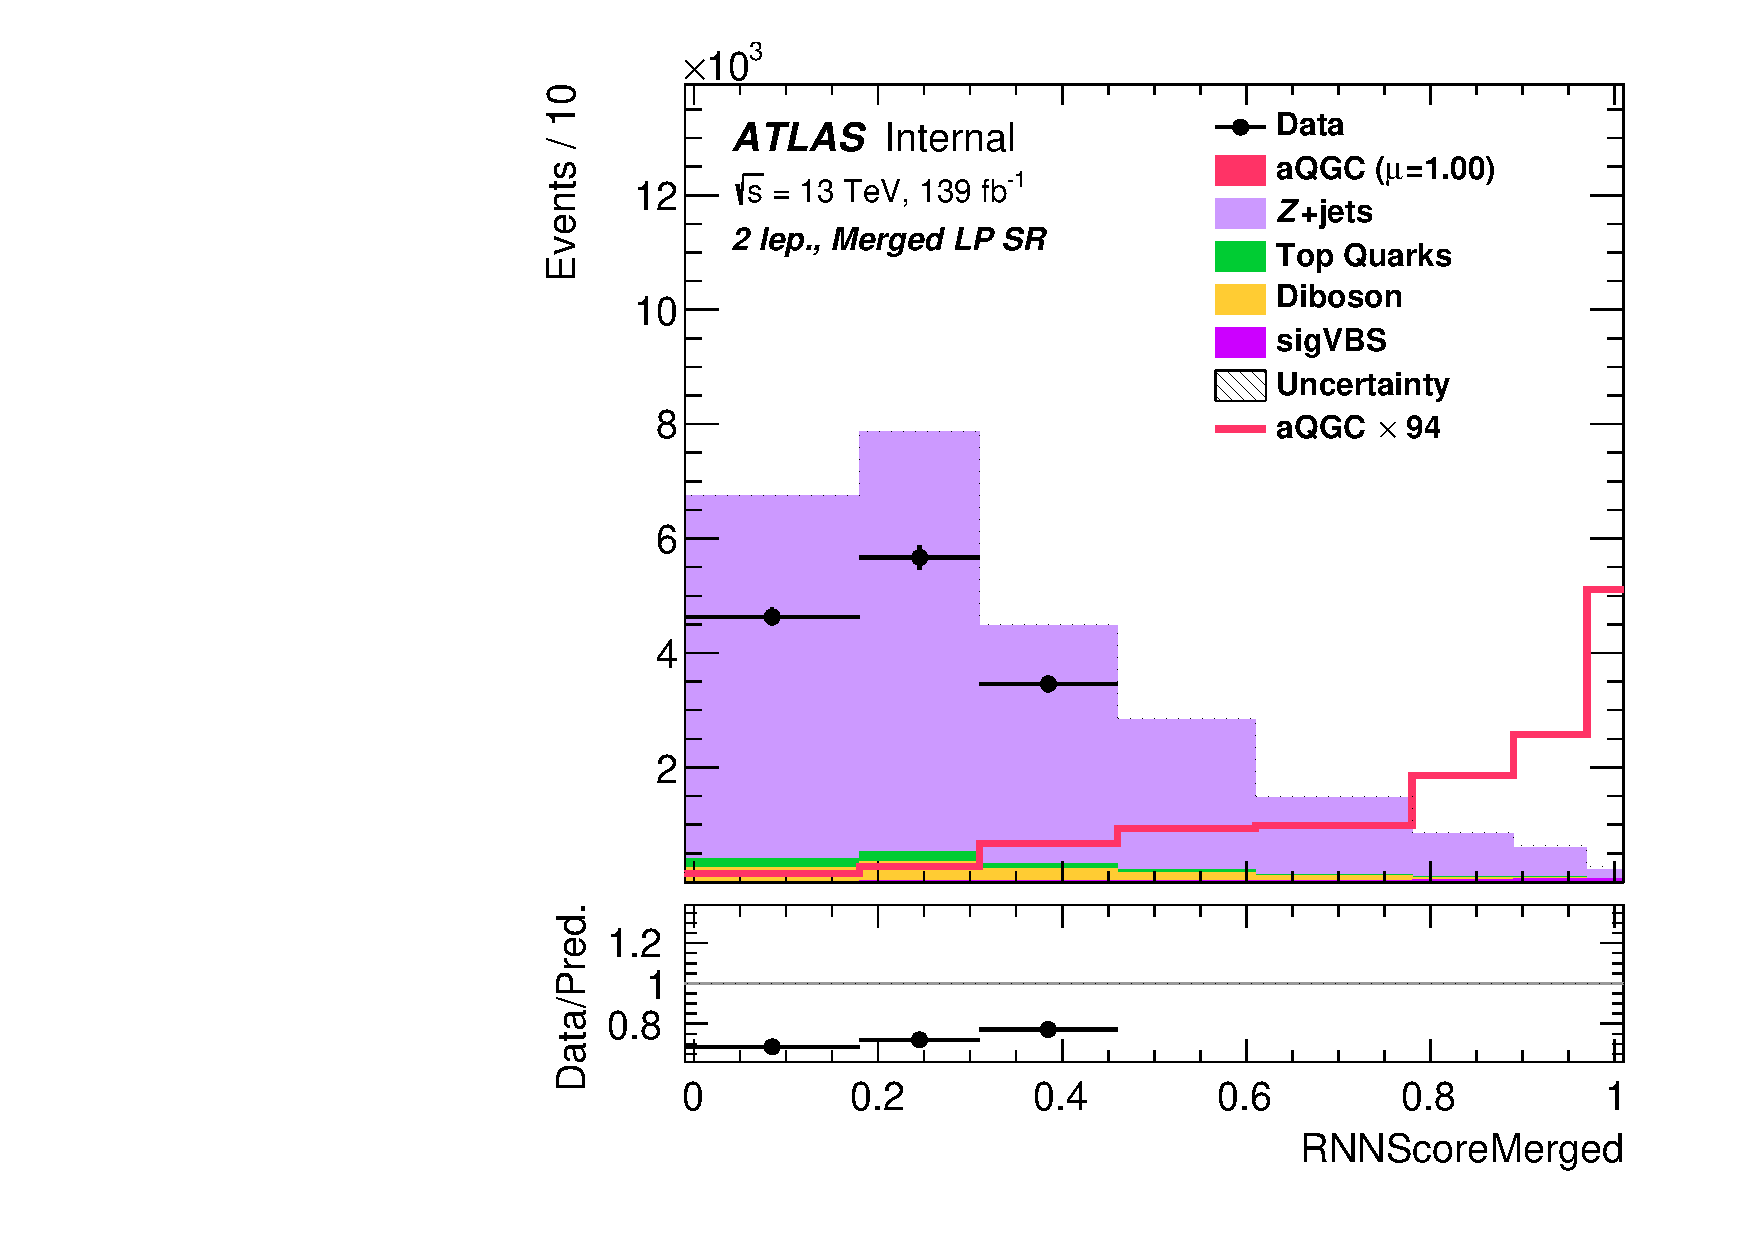
\includegraphics[width=0.32\textwidth]{figures/aQGC/Region_distRNNScoreMerged_DSRVBSLPLMVV_BMin0_J0_incJet1_L2_T0_incFat1_Y6051_incTag1_Fat1_Prefit.pdf}}
    	\subfigure[ 2lep LP HighMVV SR ]{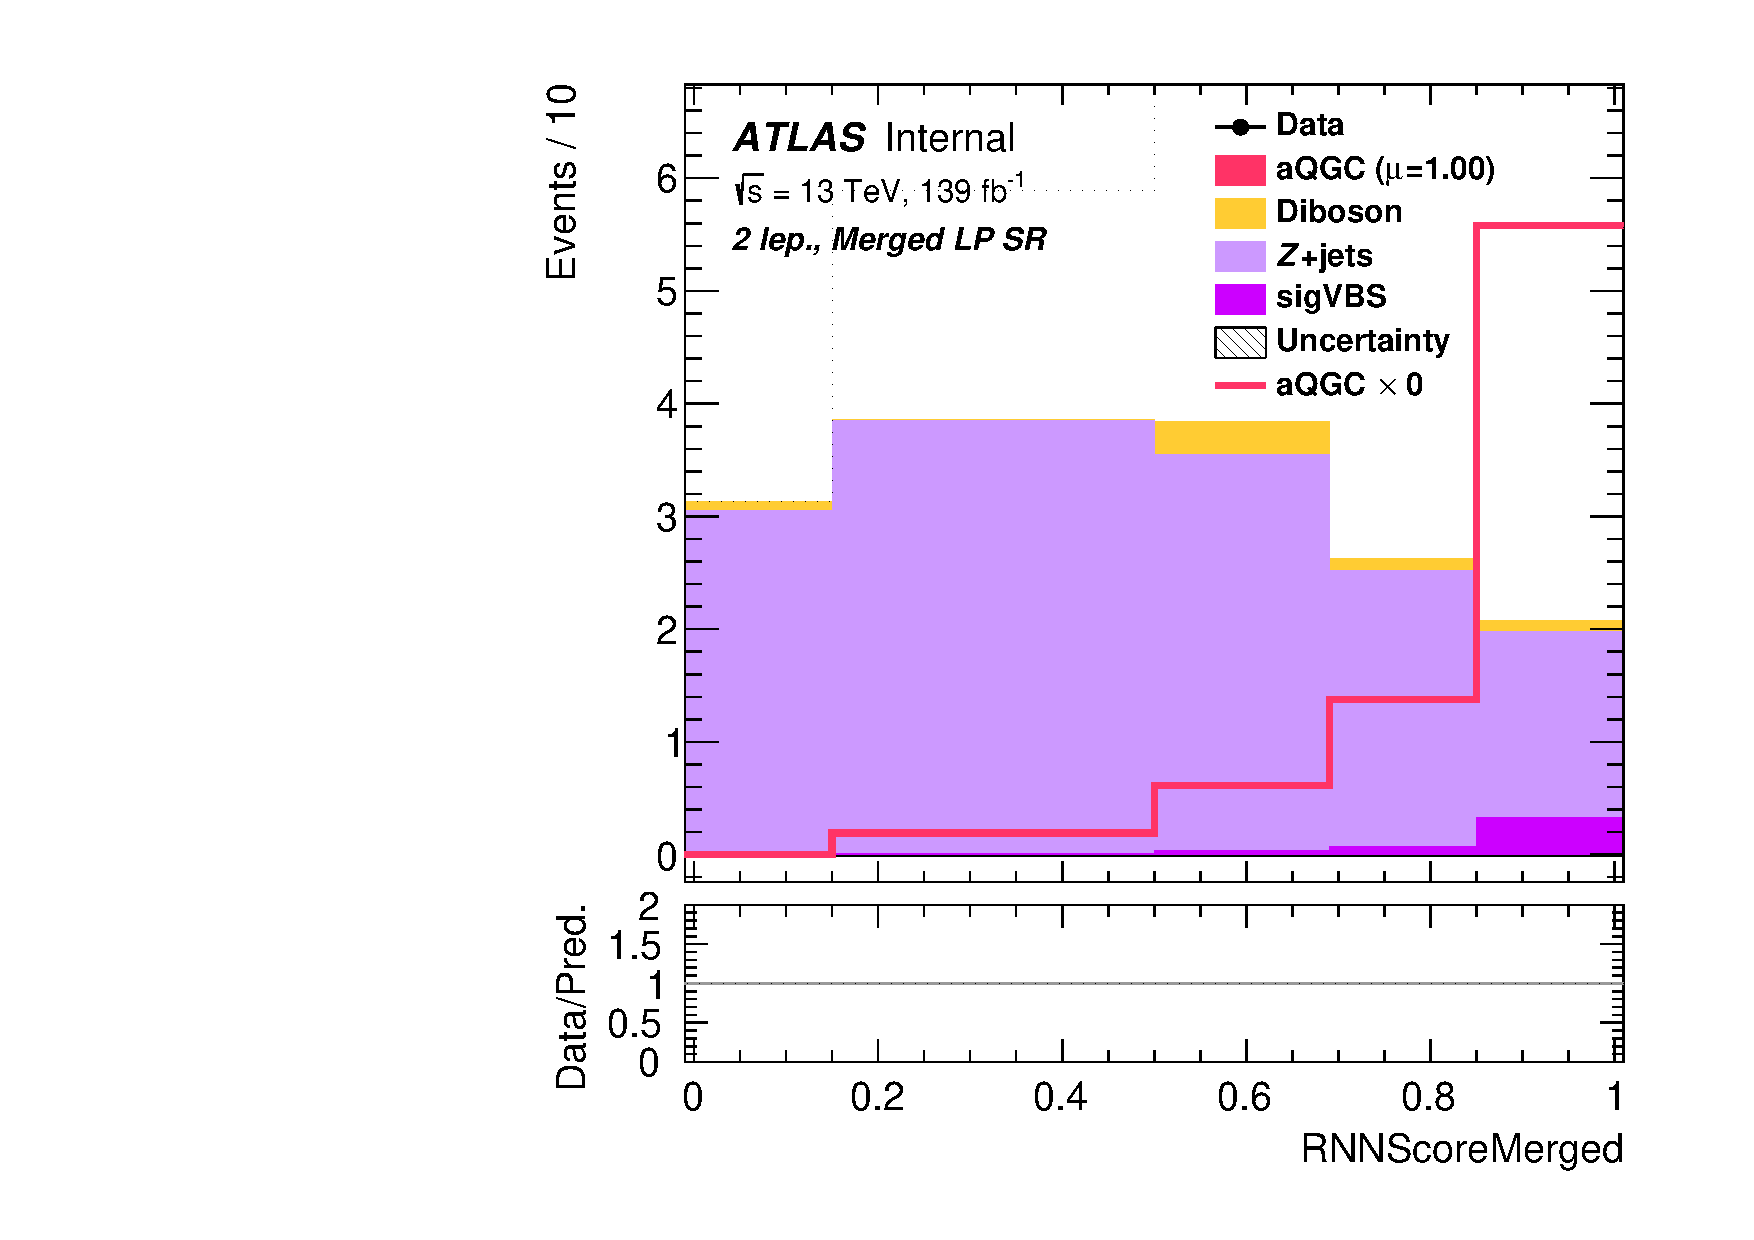
\includegraphics[width=0.32\textwidth]{figures/aQGC/Region_distRNNScoreMerged_DSRVBSLPHMVV_BMin0_J0_incJet1_L2_T0_incFat1_Y6051_incTag1_Fat1_Prefit.pdf}}
        \caption{Prefit plots for 2-bin strategy is shown. The RNN score is used as discriminant for signal regions. operator FT0 in \tlep channel are shown. The standard model EW signal is floated as the background.}
        \label{fig:2lepTwoBin}
\end{figure}

\begin{table}[ht!]
\small
\begin{center}
\resizebox{0.9\textwidth}{!}{
\begin{tabular}{ | l || l | l | l |}
                                    & single bin fit with $m_{VV}$& single bin fit with RNN  & 2-bin fit with RNN   \tabularnewline \hline
Unconditional fitted $\mu$          & -2.7e-06 $\pm$ 0.067   & 3.38e-05 $\pm0.038$      & 3.35e-05 $\pm0.029$  \tabularnewline \hline
Norm sigVBS                         & 1 $\pm$ 2.1            & 1 $\pm$ 0.94             & 1 $\pm$ 0.48         \tabularnewline \hline
Norm Z                              & 1 $\pm$ 0.036          & 1 $\pm$ 0.029            & 1 $\pm$ 0.027        \tabularnewline \hline
Norm VV                             & 1 $\pm$ 1.13           & 1 $\pm$ 0.71             & 0.99 $\pm$ 0.64      \tabularnewline \hline
Expected limit of $\mu$             & 0.19                   & 0.72                     & 0.10                 \tabularnewline \hline
Expected limit of Wilson coefficient & 0.44                   & 0.85                     & 0.32                 \tabularnewline \hline
\end{tabular}
}
\caption{Expected signal strength and limits in each two options. only \tlep channel is used for the fit. The result for single bin fit with RNN is also shown as a reference. The normarizations fitted for standard model signal, and Z and diboson backgrounds are shown as Norm in the table.}
\label{tab:2binlimit}
\end{center}
\end{table}

2-bin fit can constrain the standard model signal, as shown in the uncertainty of Norm sigVBS of table~\ref{tab:2binlimit}. 
When comparing single bin fit with $m_{VV}$ and 2-bin fit with RNN, 2-bin fit with RNN appears to be able to provide a better limit.

\subsection{Clipping method}
\label{subsec:clipping}
As the EFT violates unitarity at large energy scale, the clipping method is used to preserve the unitarity at high center of mass energies. The EFT signal is set to zero at $truth m_{VV} > E_{clip}$, where the $E_{clip}$ is [2,3,4,5,$\infty$]~TeV. 5 points are chosen as recommended from the aGC coupling taskforce.\cite{ATL-COM-PHYS-2017-433} 
The expected limit with all 3 channels with each of the clipping points are shown in figure~\ref{fig:ClippedLimits}. 
The systematic uncertainties are yet to be included and the fitting only constraints the floated normalization.
%Fitting includes all systematics uncertainties.

\begin{figure}[ht]
    \centering
    	\subfigure[ FT0 ]{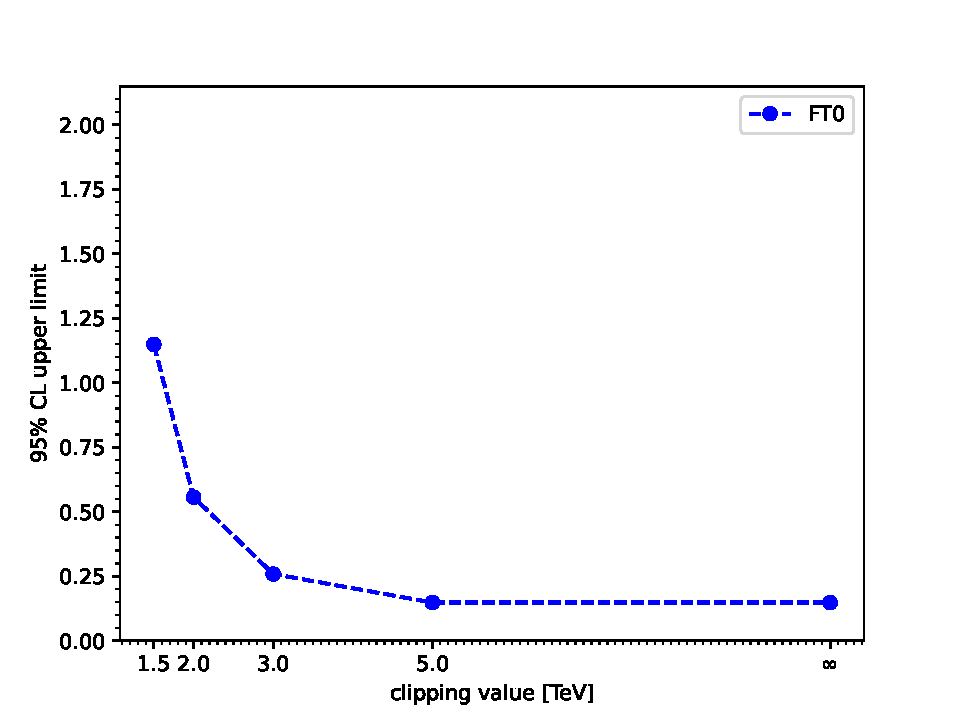
\includegraphics[width=0.32\textwidth]{figures/aQGC/ClippedFT0.pdf}}
    	\subfigure[ FT1 ]{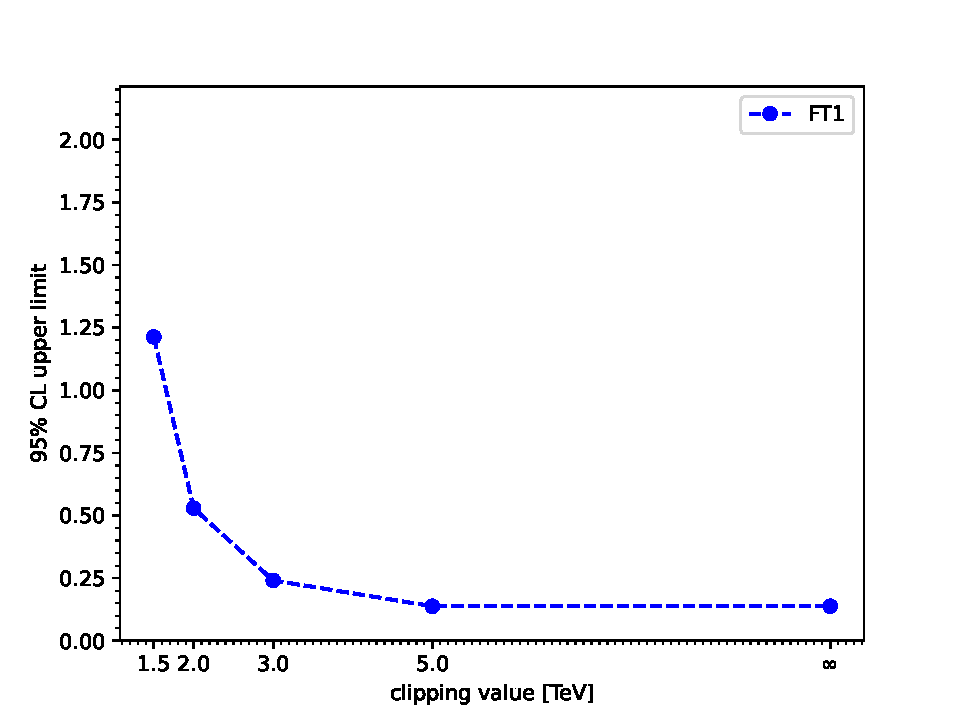
\includegraphics[width=0.32\textwidth]{figures/aQGC/ClippedFT1.pdf}}
    	\subfigure[ FT2 ]{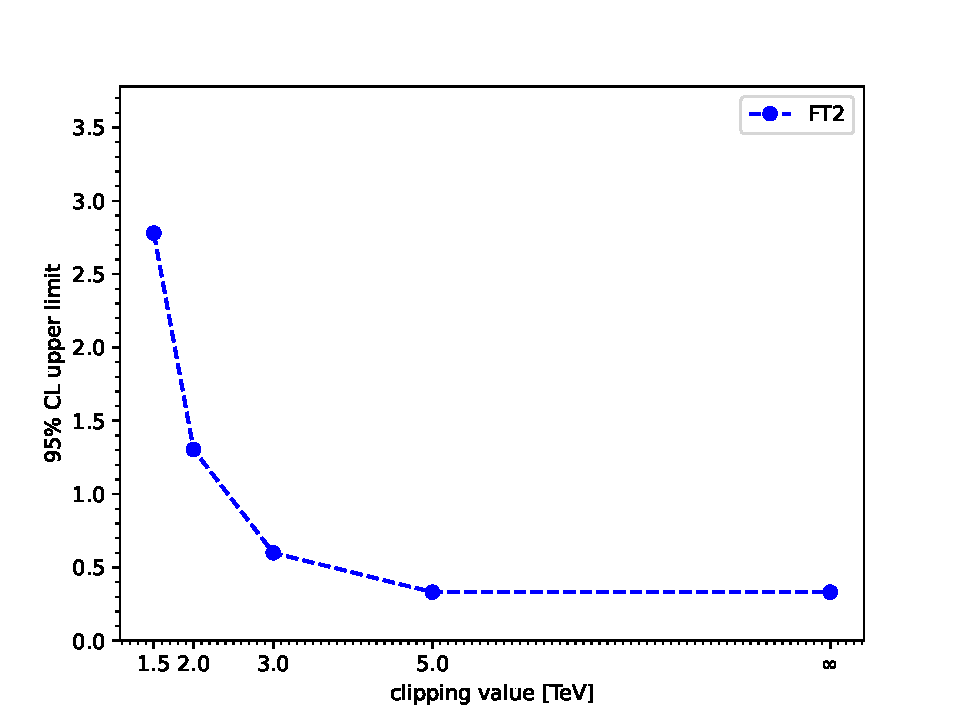
\includegraphics[width=0.32\textwidth]{figures/aQGC/ClippedFT2.pdf}}
        \caption{Expected limits for 5 clipping points are shown for each coefficient FT0, FS02, and FM0.}
        \label{fig:ClippedLimits}
\end{figure}

\begin{figure}[ht]
    \centering
    	\subfigure[ FT5 ]{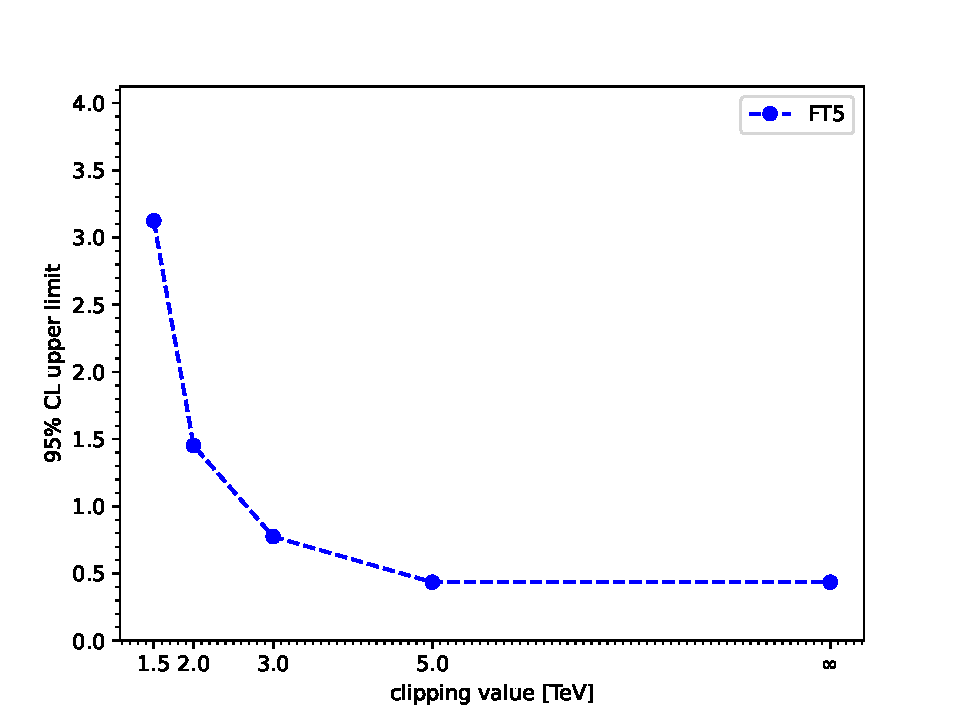
\includegraphics[width=0.32\textwidth]{figures/aQGC/ClippedFT5.pdf}}
    	\subfigure[ FT6 ]{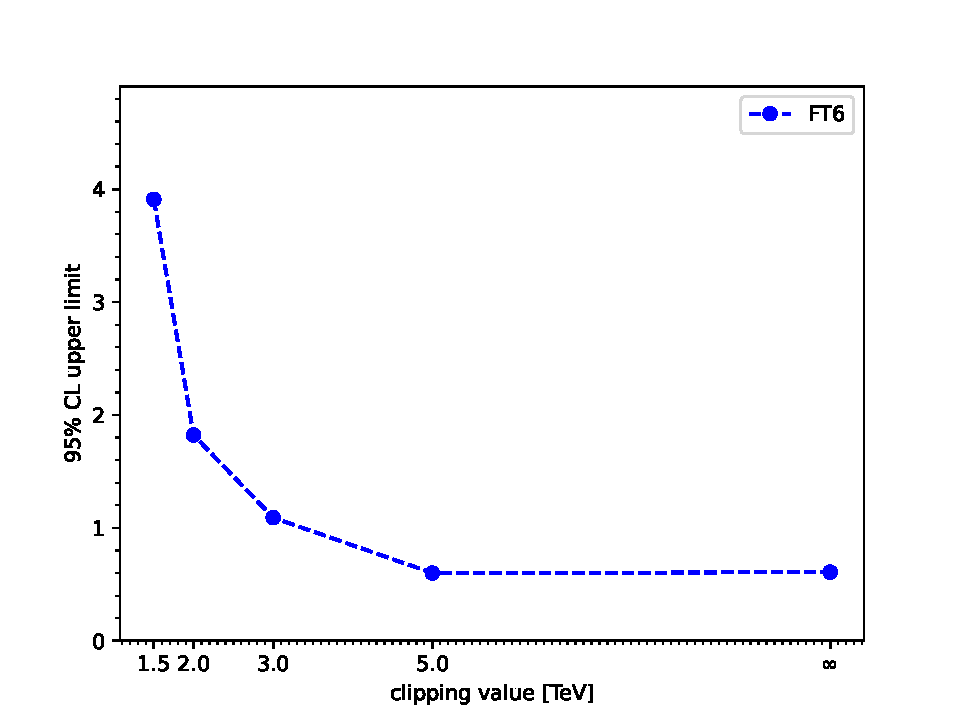
\includegraphics[width=0.32\textwidth]{figures/aQGC/ClippedFT6.pdf}}
    	\subfigure[ FT7 ]{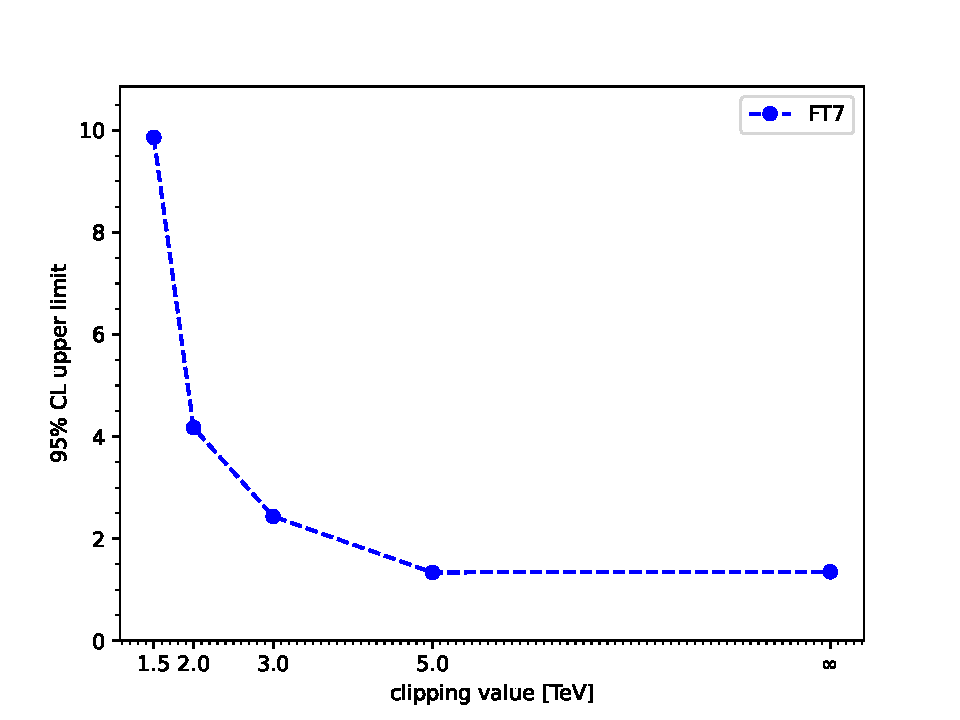
\includegraphics[width=0.32\textwidth]{figures/aQGC/ClippedFT7.pdf}}
        \caption{Expected limits for 5 clipping points are shown for each coefficient FT5, FT6, and FT7.}
\end{figure}

\begin{figure}[ht]
    \centering
    	\subfigure[ FT8 ]{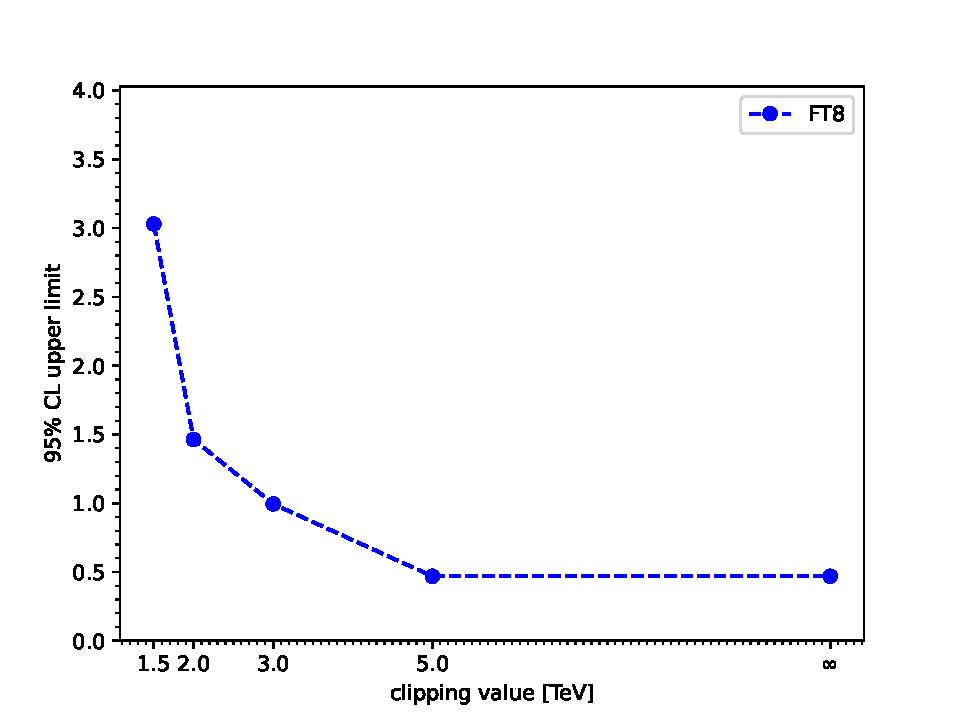
\includegraphics[width=0.32\textwidth]{figures/aQGC/ClippedFT8.pdf}}
    	\subfigure[ FT9 ]{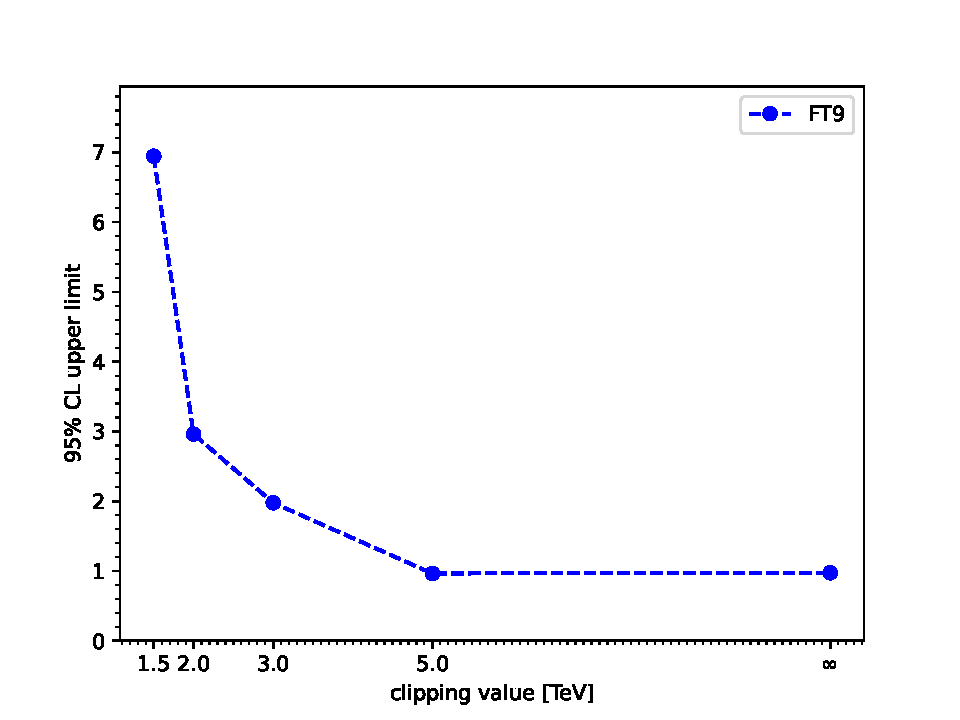
\includegraphics[width=0.32\textwidth]{figures/aQGC/ClippedFT9.pdf}}
    	\subfigure[ FM0 ]{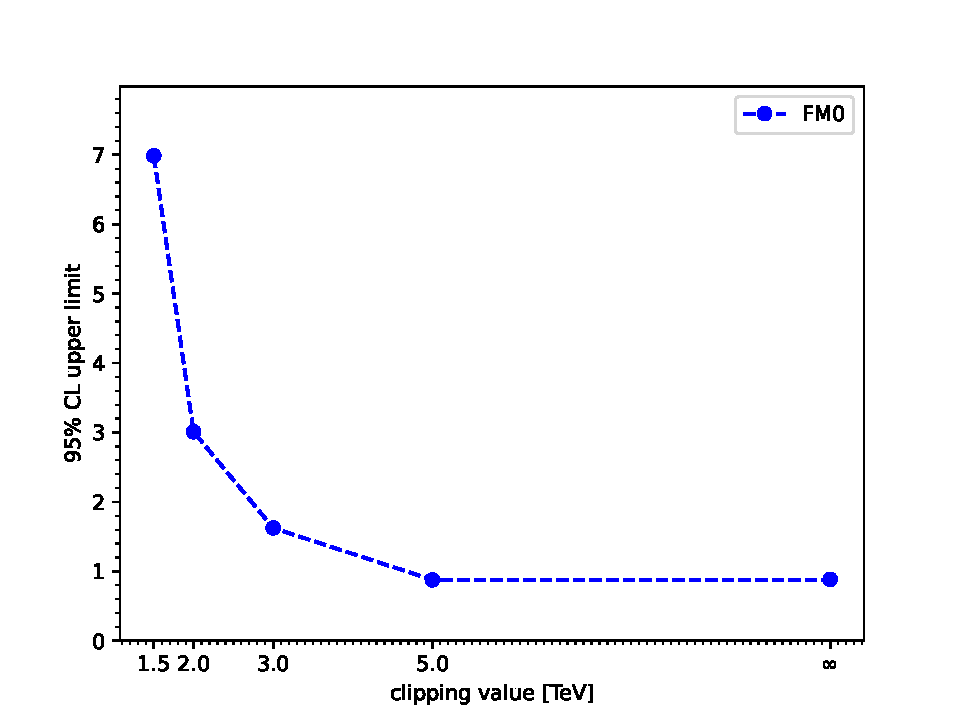
\includegraphics[width=0.32\textwidth]{figures/aQGC/ClippedFM0.pdf}}
        \caption{Expected limits for 5 clipping points are shown for each coefficient FT8, FT9, and FM0.}
\end{figure}

\begin{figure}[ht]
    \centering
    	\subfigure[ FM1 ]{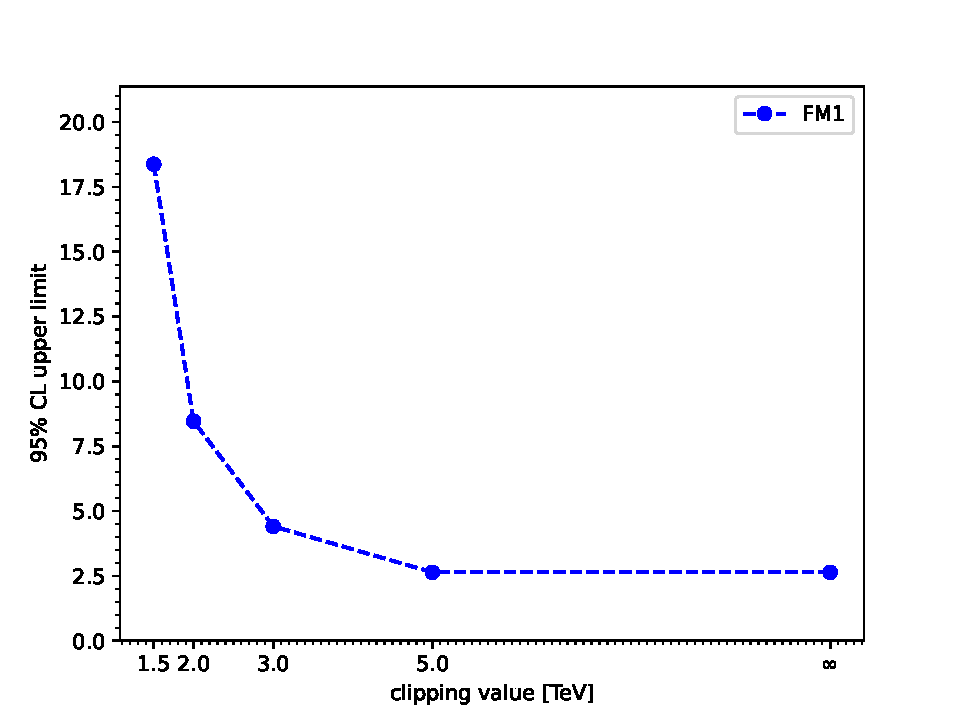
\includegraphics[width=0.32\textwidth]{figures/aQGC/ClippedFM1.pdf}}
    	\subfigure[ FM2 ]{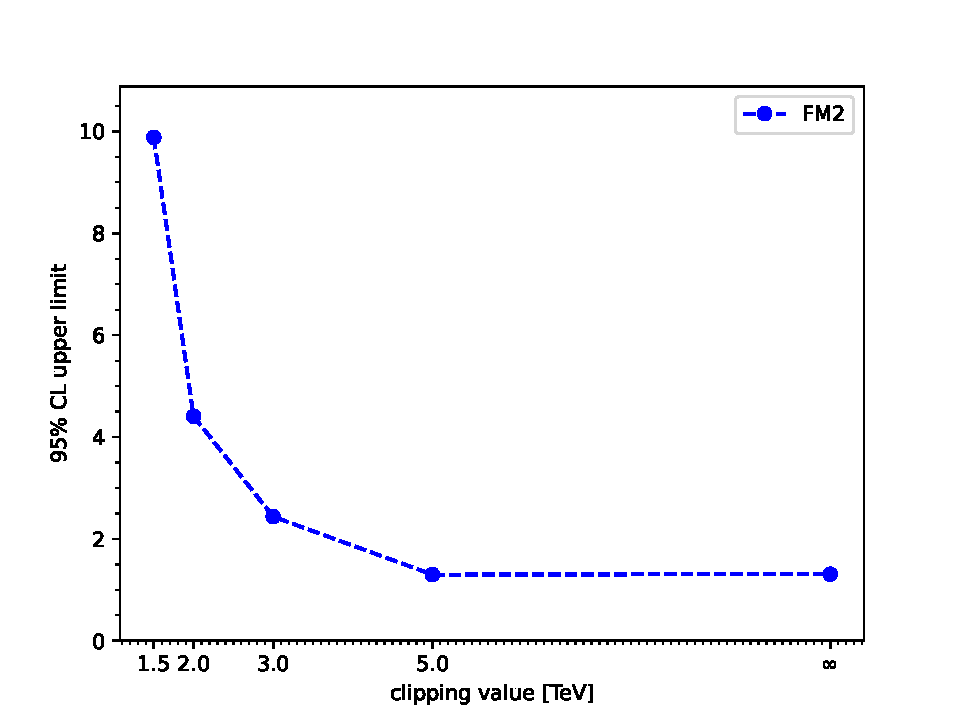
\includegraphics[width=0.32\textwidth]{figures/aQGC/ClippedFM2.pdf}}
    	\subfigure[ FM3 ]{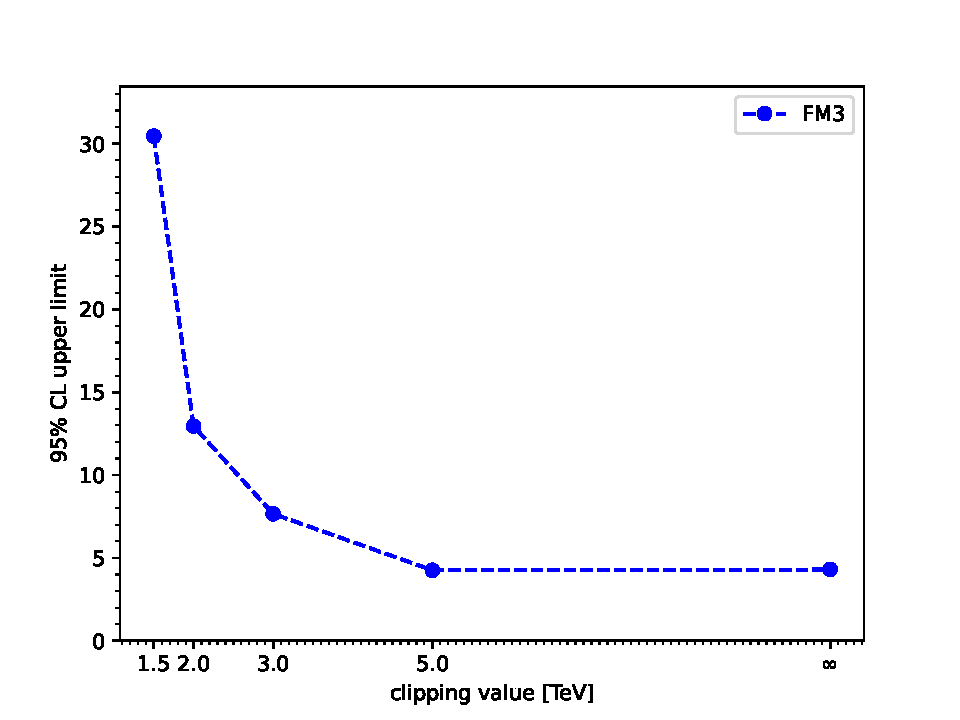
\includegraphics[width=0.32\textwidth]{figures/aQGC/ClippedFM3.pdf}}
        \caption{Expected limits for 5 clipping points are shown for each coefficient FM1, FM2, and FM3.}
\end{figure}

\begin{figure}[ht]
    \centering
    	\subfigure[ FM4 ]{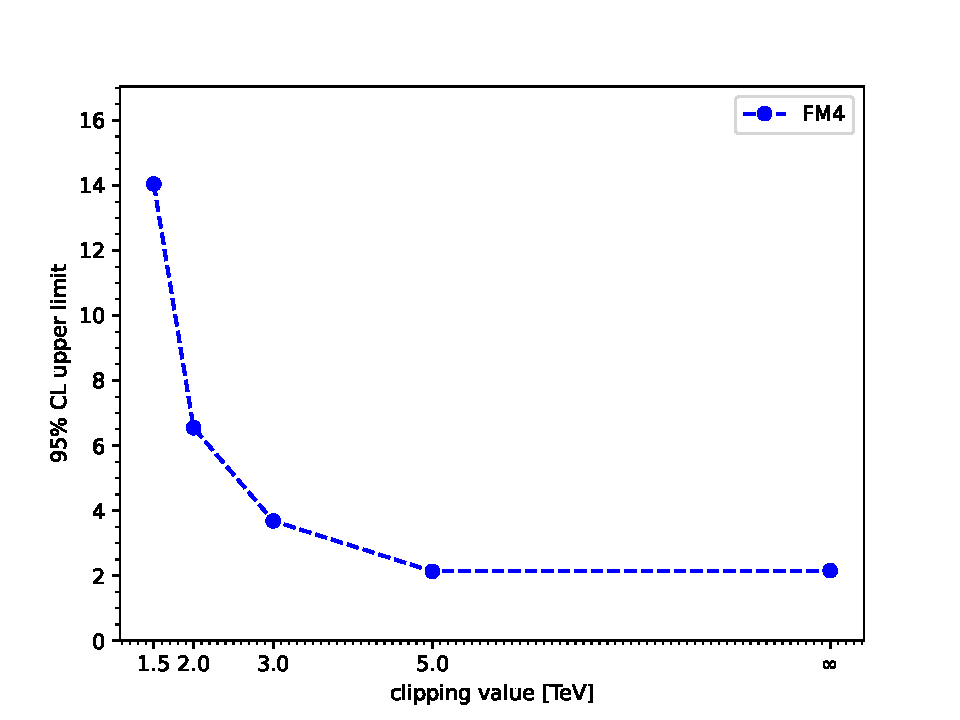
\includegraphics[width=0.32\textwidth]{figures/aQGC/ClippedFM4.pdf}}
    	\subfigure[ FM5 ]{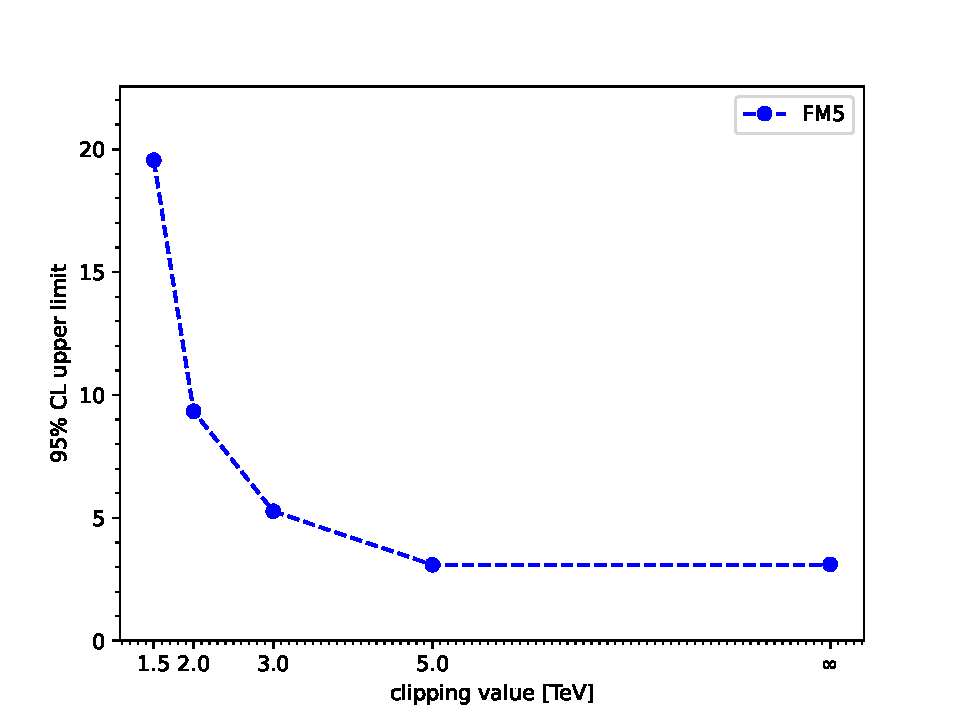
\includegraphics[width=0.32\textwidth]{figures/aQGC/ClippedFM5.pdf}}
    	\subfigure[ FM7 ]{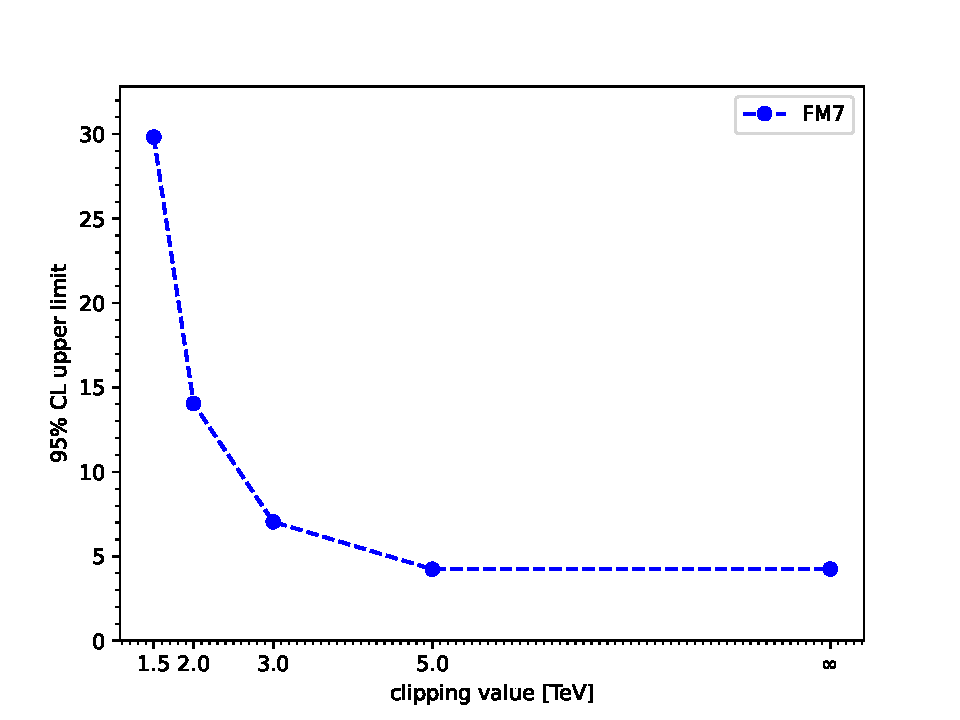
\includegraphics[width=0.32\textwidth]{figures/aQGC/ClippedFM7.pdf}}
        \caption{Expected limits for 5 clipping points are shown for each coefficient FT4, FT5, and FM7.}
\end{figure}

\begin{figure}[ht]
    \centering
    	\subfigure[ FS02 ]{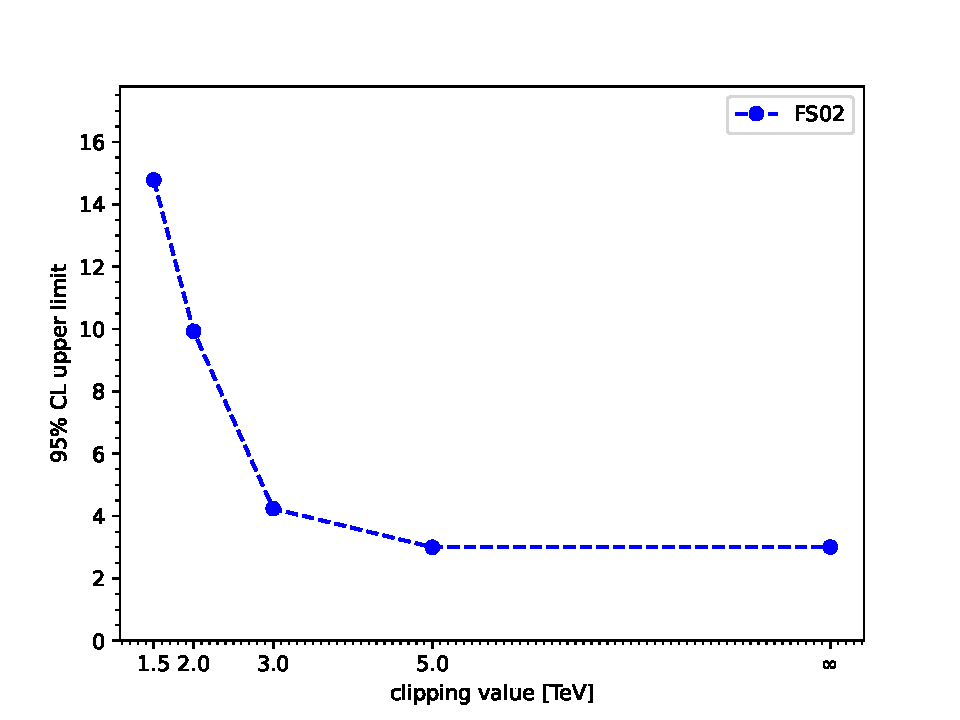
\includegraphics[width=0.32\textwidth]{figures/aQGC/ClippedFS02.pdf}}
    	\subfigure[ FS1 ]{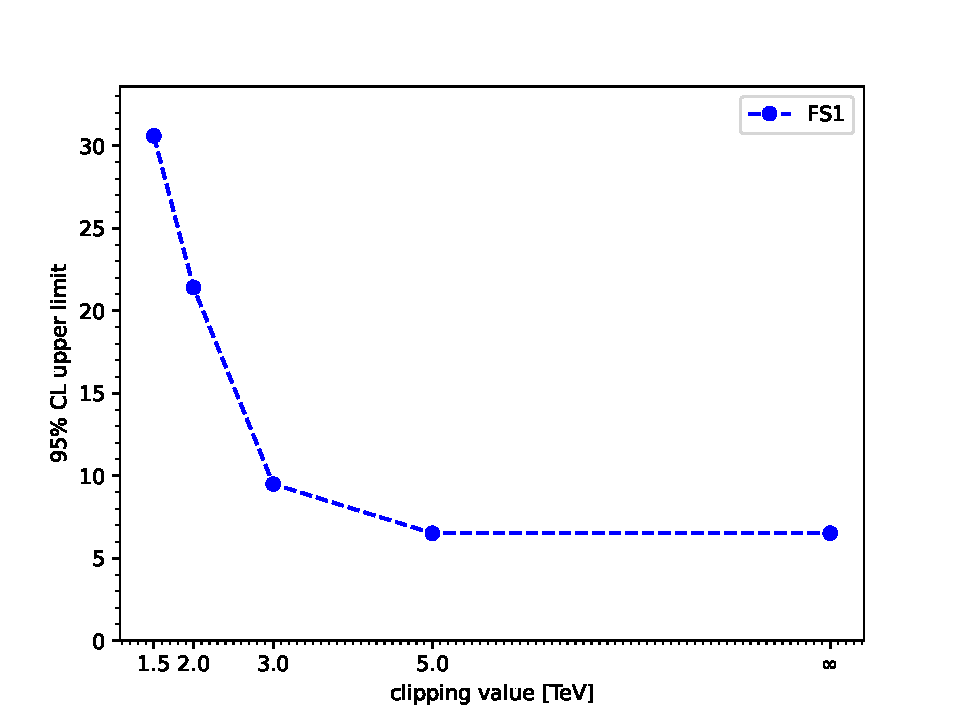
\includegraphics[width=0.32\textwidth]{figures/aQGC/ClippedFS1.pdf}}
        \caption{Expected limits for 5 clipping points are shown for each coefficient FS02, FS1.}
\end{figure}

